%=================================================================
% MDPI Mathematics — Fuzzy PSO factorial study on F1--F23
%=================================================================
\documentclass[mathematics,article,submit,pdftex,moreauthors]{Definitions/mdpi}
\usepackage{algorithm}
\usepackage{algpseudocode}
\usepackage{afterpage}
\makeatletter
\newcommand{\restoreportraitheight}{
	\global\@colht=\textheight
	\global\@colroom=\textheight
	\global\vsize=\textheight
}
\makeatother

%=================================================================
% MDPI internal commands — do not modify without reason
\firstpage{1}
\makeatletter
\setcounter{page}{\@firstpage}
\makeatother
\pubvolume{1}
\issuenum{1}
\articlenumber{0}
\pubyear{2026}
\copyrightyear{2026}
\datereceived{ }
\daterevised{ }
\dateaccepted{ }
\datepublished{ }
\hreflink{https://doi.org/}

%=================================================================
% Title / Authors
\Title{Structural Sensitivity Analysis of Fuzzy Inertia-Weight Control in Bio-Inspired Particle Swarm Optimization}
\TitleCitation{Structural Sensitivity Analysis of Fuzzy Inertia-Weight Control in Bio-Inspired Particle Swarm Optimization}

\newcommand{\orcidauthorA}{0009-0007-9934-5250} % José Barrera-García
\newcommand{\orcidauthorB}{0000-0001-5500-0188} % Broderick Crawford
\newcommand{\orcidauthorC}{0000-0002-6897-8262} % José Gómez-Pulido
\newcommand{\orcidauthorD}{0000-0001-7723-7012} % Felipe Cisternas-Caneo
\newcommand{\orcidauthorE}{0009-0000-4986-5900} % Yoslandy Lazo
\newcommand{\orcidauthorF}{0000-0002-2380-623X} % Alex Paz
\newcommand{\orcidauthorG}{0000-0003-2018-1972} % Álvaro Peña Fritz
\newcommand{\orcidauthorH}{0000-0002-5755-6929} % Ricardo Soto

\Author{José Barrera-García $^{1,2,3,*}$\orcidA{},
Broderick Crawford $^{1,*}$\orcidB{},
José Gómez-Pulido $^{2,4,5}$\orcidC{},
Felipe Cisternas-Caneo $^{4,6}$\orcidD{},
Yoslandy Lazo $^{1}$\orcidE{},
Alex Paz $^{7}$\orcidF{},
Álvaro Peña Fritz $^{7}$\orcidG{}, and
Ricardo Soto $^{1}$\orcidH{}}
\AuthorNames{José Barrera-García, Broderick Crawford, José Gómez-Pulido, Felipe Cisternas-Caneo, Yoslandy Lazo, Alex Paz, Álvaro Peña Fritz, Ricardo Soto}
\AuthorCitation{Barrera-García, J.; Crawford, B.; Gómez-Pulido, J.; Cisternas-Caneo, F.; Lazo, Y.; Paz, A.; Peña Fritz, Á.; Soto, R.}

\address{%
$^{1}$ \quad Escuela de Ingeniería Informática, Pontificia Universidad Católica de Valparaíso, Avenida Brasil 2241, Valparaíso 2362807, Chile; jose.barrera@pucv.cl (J.B.-G.); broderick.crawford@pucv.cl (B.C.); yoslandy.lazo@pucv.cl (Y.L.); ricardo.soto@pucv.cl (R.S.)\\
$^{2}$ \quad Department of Computer Science, Universidad de Alcalá, 28805 Alcalá de Henares, Spain; jose.gomez@uah.es (J.G.-P.)\\
$^{3}$ \quad Escuela de Negocios y Economía, Pontificia Universidad Católica de Valparaíso, Amunátegui 1838, Viña del Mar 2580129, Chile\\
$^{4}$ \quad Health Computing and Intelligent Systems Research Group (HCIS), Universidad de Alcalá, 28805 Alcalá de Henares, Madrid, Spain\\
$^{5}$ \quad Ramón y Cajal Institute for Health Research (IRYCIS), Madrid, Spain\\
$^{6}$ \quad Departamento de Ingeniería Industrial, Facultad de Ingeniería, Universidad del Bío-Bío, Avda. Collao 1202, Casilla 5-C, Concepción 4051381, Región del Biobío, Chile; fcisternas@ubiobio.cl (F.C.-C.)\\
$^{7}$ \quad Escuela de Ingeniería en Construcción y Transporte, Pontificia Universidad Católica de Valparaíso, Avenida Brasil 2147, Valparaíso 2362804, Chile; alex.paz@pucv.cl (A.P.); alvaro.pena@ucv.cl (Á.P.F.)}

\corres{Correspondence: Broderick Crawford (broderick.crawford@pucv.cl); José Barrera-García (jose.barrera@pucv.cl)}

%=================================================================
% Abstract & keywords
\abstract{The performance of fuzzy-controlled particle swarm optimization (PSO\_FCS) depends on the structure of its inference system, yet the influence of linguistic granularity and rule-base design remains insufficiently characterized. This study investigates the sensitivity of inertia-weight control to these structural choices using a static Mamdani fuzzy controller. A factorial comparison considers four linguistic granularities and eight systematically generated rule-base patterns, yielding 32 fuzzy configurations evaluated against classical PSO. Experiments comprise 63,426 independent runs across 62 function--dimension instances from the classical F1--F23 benchmark suite. The results reveal substantial differences among rule-base patterns, whereas increasing linguistic granularity does not consistently improve performance or reduce the dispersion between patterns. The best-ranked configuration, FCS-3-R1, achieves a mean Friedman rank of 4.77, compared with 6.36 for classical PSO, although both belong to the same Nemenyi critical-difference group. Performance rankings also differ between scalable and fixed-dimensional benchmark subsets, indicating that the preferred configuration depends on the evaluated problem set. A formal characterization establishes that four pairs of rule bases generate complementary inertia-control surfaces under the specified Mamdani inference architecture, without implying equivalent optimization performance. These findings demonstrate the importance of rule-base structure in fuzzy inertia control and provide a mathematical and empirical basis for examining structural configuration choices in PSO.}

\keyword{fuzzy control; swarm intelligence; particle swarm optimization; linguistic granularity; rule-base structure; Mamdani inference}

% Compatibility shim for the MDPI marginfix package with older LaTeX kernels.
\providecommand{\UseTaggingSocket}[1]{}

%%%%%%%%%%%%%%%%%%%%%%%%%%%%%%%%%%%%%%%%%%
\begin{document}

%%%%%%%%%%%%%%%%%%%%%%%%%%%%%%%%%%%%%%%%%%
\section{Introduction}
\label{sec:introduction}

% Particle swarm optimization (PSO) is a bio-inspired, population-based stochastic optimizer rooted in swarm intelligence, in which particles update their positions using individual and collective search experience \cite{KennedyEberhart1995}. The inertia weight scales the previous velocity and helps regulate the balance between exploration and exploitation \cite{ShiEberhart1998}. A fuzzy control system (FCS) can adjust this weight during the search using measures of optimization progress \cite{ShiEberhart2001}. Research on evolved fuzzy feedback policies further illustrates the scope for state-dependent parameter control \cite{Roy2024}. Within this swarm-intelligence framework, fuzzy partitions and the rule base determine how observations of the search process are translated into a control action.


Particle swarm optimization (PSO) is a bio-inspired, population-based stochastic optimization algorithm rooted in swarm intelligence, in which particles update their positions using individual and collective search experience \cite{KennedyEberhart1995}. The inertia weight regulates the influence of previous velocities and plays an important role in balancing exploration and exploitation during the search \cite{ShiEberhart1998}. Integrating fuzzy logic with bio-inspired optimization provides a means of regulating this search behavior through linguistic rules that map information about the optimization process into parameter adjustments. In PSO, a fuzzy control system (FCS) can regulate the inertia weight using measures of search progress and population diversity \cite{ShiEberhart2001}. Research on evolved fuzzy feedback policies further illustrates the potential of state-dependent parameter control \cite{Roy2024}. Within this integration, linguistic partitions and rule-base structure determine how the observed search state is translated into an inertia-control action.


In a Mamdani fuzzy inference system (FIS), the antecedents and consequents of linguistic rules are represented by fuzzy sets \cite{Gacto2011}. Linguistic granularity is a substantive design choice in fuzzy modeling, with implications for partition resolution, rule-base complexity, and interpretability \cite{Castiello2019,Gacto2011}. For the controller studied here, the number $n$ of linguistic labels determines the resolution of both input and output partitions, while the rule base maps combinations of diversity and iteration progress to an inertia weight. These are distinct but coupled structural choices: for a complete two-input table with equal granularity, increasing $n$ from 3 to 9 raises the rule count from 9 to 81. Whether finer partitions improve PSO performance therefore requires empirical assessment, rather than being inferred from representational resolution alone.

% The specific question addressed here is how the performance of a static Mamdani inertia controller varies with linguistic granularity and rule-base pattern when the inference architecture and optimization budget are held fixed. This complements research on fuzzy parameter control and partition design by comparing complete controller configurations under common experimental conditions. The study evaluates 32 PSO\_FCS configurations formed by four granularities and eight rule-base patterns across the Classical Benchmark Suite F1--F23, using classical PSO as a baseline. It characterizes ranking and dynamic variation across functions and benchmark groups, rather than introducing a new optimizer or an adaptive selector. Because changing granularity also changes the rule-table size, the comparison does not isolate granularity and rule structure as independent causal effects.


The specific question addressed here is how linguistic granularity and rule-base structure influence the behavior and optimization performance of a static Mamdani fuzzy inertia controller within a bio-inspired search algorithm. By examining these structural design choices under a common inference architecture and optimization budget, the study seeks to provide mathematical and empirical evidence to inform the design of fuzzy control systems for PSO. Specifically, 32 PSO\_FCS configurations, combining four linguistic granularities and eight rule-base patterns, are evaluated across the Classical Benchmark Suite F1--F23, using classical PSO as a baseline. The analysis examines differences in optimization performance, configuration rankings, and controller dynamics across benchmark functions and problem groups. Rather than introducing a new optimizer or an online configuration selector, the study characterizes the behavior of predefined controller structures. Since increasing linguistic granularity also changes the number of rules, the comparisons concern complete configurations and do not establish independent causal effects of granularity and rule-base structure.


% The contributions of this work are:
% \begin{enumerate}
% 	\item an explicit parametric specification of a static Mamdani FCS, including its generated linguistic partitions and rule-base pattern families;
% 	\item a mathematical characterization of the mirror symmetry satisfied by designated rule-pattern pairs under the specified inference architecture;
% 	\item a controlled factorial comparison of four granularities and eight consequent patterns under a common PSO implementation and experimental budget, supported by supplementary run-level data and machine-readable statistical summaries; and
% 	\item empirical evidence of ranking and dynamic heterogeneity among the evaluated configurations across functions and benchmark groups.
% \end{enumerate}


The main contributions of this work are:
\begin{enumerate}
    \item A parametric formulation of a static Mamdani fuzzy inertia controller for bio-inspired optimization, defining linguistic partitions and systematically generated rule-base families to examine how structural design choices shape the control of PSO search behavior;

    \item A formal characterization of mirror symmetry between designated rule-base patterns, establishing conditions under which their induced inertia-control surfaces are complementary and providing a mathematical basis for comparing structurally related fuzzy controllers;

    \item A controlled factorial evaluation of four linguistic granularities and eight rule-base patterns under a common PSO implementation and computational budget, supported by supplementary run-level data and machine-readable statistical summaries;

    \item Empirical evidence that increasing linguistic granularity does not consistently improve optimization performance or reduce differences among rule-base patterns, highlighting the importance of rule-base structure and the dependence of configuration rankings and controller behavior on the evaluated optimization problems.
\end{enumerate}


The remainder of the paper is organized as follows. Section~\ref{sec:related_work} reviews prior work; Section~\ref{sec:framework} introduces the parametric controller and formalizes its rule-base families; Section~\ref{sec:experimental_design} describes the experimental protocol; Section~\ref{sec:results} reports global, function- and problem-class rankings, rule-base and granularity comparisons, robustness and dimensional scaling, and controller dynamics; and Sections~\ref{sec:discussion} and~\ref{sec:conclusion} interpret the findings and summarize the conclusions and future work.

%%%%%%%%%%%%%%%%%%%%%%%%%%%%%%%%%%%%%%%%%%
\section{Related Work}
\label{sec:related_work}

\subsection{Inertia-Weight Control in Particle Swarm Optimization}
\label{subsec:pso_inertia}

PSO is a population-based stochastic optimizer in which each particle combines inertia with cognitive and social attraction terms \cite{KennedyEberhart1995}. The inertia weight $w$ directly scales the previous velocity; it is therefore a principal mechanism for controlling the exploration--exploitation balance. The original and early variants used a constant coefficient, whereas the widely used linearly decreasing inertia-weight schedule explicitly changes search behavior over the optimization horizon \cite{ShiEberhart1998}. Subsequent work has investigated nonlinear schedules \cite{Chatterjee2006}, feedback from swarm success \cite{Nickabadi2011}, stability-aware adaptation \cite{Taherkhani2015}, and joint adaptation of inertia and acceleration coefficients \cite{Duan2022,Han2024}.

This body of work establishes an important distinction. A time-indexed schedule changes $w$ but does not observe the current search state. State-dependent controllers instead use quantities such as diversity, improvement, distance, or stagnation to react to the population trajectory \cite{Nickabadi2011,Taherkhani2015}. Such feedback is particularly relevant because benchmark landscapes differ substantially in modality and conditioning; a search policy suitable for rapid local refinement need not be suitable for maintaining diversity in a multimodal landscape. The question addressed here is more specific: once a fuzzy state-feedback controller has been selected, how sensitive is its behavior to the semantic resolution of its partitions and to its rule-base structure?

\subsection{Fuzzy State-Feedback Control of PSO Parameters}
\label{subsec:fuzzy_pso}

A fuzzy inference system (FIS) provides an interpretable way to map numerical state descriptors into a control action. In a Mamdani FIS, linguistic antecedents and consequents are combined through a rule base and a defuzzification operator; this architecture remains a canonical model-free fuzzy-control paradigm \cite{Mamdani1974,Lee1990,Nguyen2019Fuzzy}. When used in PSO, the inputs commonly represent population diversity, iteration progress, or an improvement signal, and the output is an adapted value of $w$ or of several PSO coefficients \cite{ShiEberhart2001,Nobile2018,Valdez2017}.

Fuzzy-PSO studies address different control targets and design questions. Valdez et al. compared fuzzy-logic augmentation across PSO variants for mathematical functions using co-evolution \cite{Valdez2017}. Xia et al. designed a multiple-input multiple-output fuzzy controller to tune adaptive learning weights \cite{Xia2023}, while Roy et al. developed benchmark-trained fuzzy feedback policies and reported 127 PSO algorithm variants with up to seven controlled parameters \cite{Roy2024}; the latter article was published in 2025. Salimi et al. applied fuzzy-adaptive PSO to reachability analysis in systems specified through graph transformations \cite{Salimi2025}, a distinct application domain. These contributions demonstrate the breadth of fuzzy parameter control, but they do not change the question addressed here: sensitivity of a fixed static Mamdani inertia architecture to granularity and consequent-pattern choices.

\subsection{Fuzzy Partitions, Linguistic Granularity, and Interpretability}
\label{subsec:granularity}

Linguistic granularity is the number of labels used to discretize a fuzzy universe. It is not merely an implementation detail: it determines which distinctions the controller can express and, for a multi-input rule base, determines the number of candidate rules. A well-formed fuzzy partition is expected to provide coverage, normality, distinguishability, and a semantically ordered set of labels \cite{Klir2005,DuboisPrade2000}. Uniform triangular Ruspini partitions are a common construction because adjacent sets overlap smoothly while their membership grades sum to one over the normalized domain.

The accuracy--interpretability trade-off associated with granularity has long been recognized in fuzzy modeling. Fine partitions can represent smaller input distinctions, but expand the potential rule base; coarser partitions reduce complexity at the cost of local resolution. Gacto et al. review measures for interpretability in linguistic fuzzy rule-based systems \cite{Gacto2011}, while Castiello et al. study variable-granularity interpretable partitions for classified data \cite{Castiello2019}. These works motivate treating granularity as a structural design choice, but they do not make optimization performance a direct measure of interpretability. For the present controller, the number of labels and consequent mapping are separate, coupled choices.

Rule-base design is a second, distinct source of semantic variation. Fuzzy-system design methods can tune membership parameters, induce or prune rules, or modify the partition itself \cite{Ojha2019,Gu2022}. Evolving systems may split rules in response to drift \cite{Lughofer2018} or derive interpretable partitions from observed data \cite{Guillaume2004}. Such adaptive approaches are valuable, but they do not identify whether a particular static combination of granularity and rule logic generalizes over qualitatively different optimization landscapes. Establishing that baseline is necessary before attributing an advantage to more elaborate structural adaptation.

\subsection{From Structural Adaptation to Configuration Selection}
\label{subsec:structural_adaptation}

The broader fuzzy-systems literature distinguishes parameter adaptation from structural adaptation. The former changes membership-function parameters or rule weights; the latter may add, split, merge, or remove rules and partition elements \cite{Gu2022,Saad2020}. Recent research further investigates interpretable evolving partitions \cite{Lughofer2018}, semantic constraints during evolutionary controller design \cite{Megherbi2019}, and variable-granularity knowledge representations \cite{Ahmed2017}. These strands demonstrate that fuzzy semantics need not be treated as immutable.

Nevertheless, the flexibility of an adaptive mechanism can make interpretation difficult when multiple semantic choices change together. A controlled comparison of static configurations provides complementary descriptive evidence about how rankings vary when granularity and rule patterns are changed under a common architecture. Such comparisons do not by themselves identify independent causal effects or confirm a factorial interaction.

\subsection{Research Gap and Positioning of This Study}
\label{subsec:positioning}

Prior fuzzy-PSO studies demonstrate feedback controllers, multi-parameter adaptation, and optimized fuzzy policies, while fuzzy-modeling research treats partition granularity and interpretability as substantive design concerns. The present study is positioned as a controlled structural sensitivity analysis of a static Mamdani fuzzy inertia controller, not as a claim that no earlier factorial study exists. It evaluates four granularities, $n \in \{3,5,7,9\}$, and eight generated consequent patterns, $R_1,\ldots,R_8$, under common inputs, membership-function family, inference method, PSO implementation, and experimental budget. Because granularity changes both partition resolution and rule-table size, the results compare complete configurations rather than identify independent causal effects. The analysis also examines whether performance dispersion among rule-base patterns changes consistently across linguistic granularities, providing descriptive evidence on the sensitivity of complete controller configurations. The study does not validate an adaptive selector.

%%%%%%%%%%%%%%%%%%%%%%%%%%%%%%%%%%%%%%%%%%
\section{Parametric Fuzzy Inertia Controller}
\label{sec:framework}

This section defines the static fuzzy-control component used by all PSO\_FCS variants. The controller receives normalized diversity and iteration progress and returns an inertia weight bounded by $[w_{\min},w_{\max}]$.

\subsection{Mamdani FIS design}
\label{subsec:fis_design}

The two inputs are the diversity ratio $d_t \in [0,1]$ and normalized progress $p_t \in [0,1]$. The output universe is normalized to $[0,1]$ and is linearly rescaled to $[w_{\min},w_{\max}]$ after defuzzification. For each evaluated granularity $n \in \{3,5,7,9\}$, let $\mathcal{L}_n=\{0,\ldots,n-1\}$ index the labels. Each input and output partition is uniform triangular with overlap one and shoulders at the boundaries, satisfying $\sum_{i\in\mathcal{L}_n}\mu_i(x)=1$ on $[0,1]$. The indices $i,j,k\in\mathcal{L}_n$ denote diversity, progress, and output labels; $\mu_i^D$, $\mu_j^P$, and $\mu_k^W$ are their membership functions. For selected pattern $R\in\{R1,\ldots,R8\}$, $k_R(i,j)\in\mathcal{L}_n$ is the consequent index assigned to antecedent pair $(i,j)$.

Figure~\ref{fig:mf_inputs} shows the two I1 input partitions and Figure~\ref{fig:mf_output} shows the O1 output partition for all four granularities. Increasing $n$ narrows the support of each label and refines the controller's resolution; the Ruspini property and boundary shoulders are preserved.

\begin{figure}[H]
\begin{adjustwidth}{-\extralength}{0cm}
	\centering
	\includegraphics[width=\fulllength]{figures/06_input_diversity_mf_panel_I1.png}
	\par\smallskip
	\includegraphics[width=\fulllength]{figures/07_input_progress_mf_panel_I1.png}
\end{adjustwidth}
	\caption{I1 input membership functions for $n\in\{3,5,7,9\}$. Top: normalized swarm diversity; bottom: iteration progress. Each panel shows all four granularities.}
	\label{fig:mf_inputs}
\end{figure}

\begin{figure}[H]
\begin{adjustwidth}{-\extralength}{0cm}
	\centering
	\includegraphics[width=\fulllength]{figures/08_output_w_mf_panel.png}
\end{adjustwidth}
	\caption{O1 output membership functions for $n\in\{3,5,7,9\}$ on the normalized universe $[0,1]$. The defuzzified centroid is rescaled to $[w_{\min},w_{\max}]=[0.1,0.9]$.}
	\label{fig:mf_output}
\end{figure}

For antecedent pair $(i,j)$, the firing strength is
\begin{equation}
\alpha_{ij}=\min\{\mu_i^D(d_t),\mu_j^P(p_t)\}.
\end{equation}
Mamdani implication clips each consequent membership function and max aggregation gives
\begin{equation}
\mu_{\mathrm{agg}}(z)=\max_{i,j}\min\{\alpha_{ij},\mu^W_{k_R(i,j)}(z)\}.
\end{equation}
The aggregated membership function is defined over $z\in[0,1]$, and the raw output is its centroid. In the implementation, the integral is approximated by trapezoidal quadrature on a 501-point grid; the raw centroid is normalized using the minimum and maximum centroids of the output sets before affine rescaling:
\begin{equation}
\begin{aligned}
\bar z_t &= \frac{\int_0^1 z\,\mu_{\mathrm{agg}}(z)\,dz}{\int_0^1 \mu_{\mathrm{agg}}(z)\,dz},\\
\widetilde z_t &= \operatorname{clip}\!\left(\frac{\bar z_t-z^c_{\min}}{z^c_{\max}-z^c_{\min}},0,1\right),\\
w_t &= w_{\min}+\widetilde z_t(w_{\max}-w_{\min}).
\end{aligned}
\end{equation}
Here $z^c_{\min}$ and $z^c_{\max}$ are the smallest and largest centroids of the output membership functions. If the aggregated area is at most $10^{-12}$, the implementation uses raw centroid fallback $\bar z_t=0.5$ before applying the same centroid-bound normalization. For this experiment, $w_{\min}=0.1$ and $w_{\max}=0.9$.

\subsection{Rule bank R1--R8}
\label{subsec:rules}

The rule bank contains eight fixed patterns representing the admissible directional relationships between diversity, progress, and the output inertia weight. Each pattern is generated algorithmically for arbitrary $n$; no rule matrix is manually rewritten for a particular granularity. A configuration is therefore identified by the pair $(n,R)$, with $n \in \{3,5,7,9\}$ and $R \in \{R1,\ldots,R8\}$.

The rule generator produces $n^2$ consequents for every pattern. The resulting matrices are validated for cardinality, deterministic generation, and bounded output. Figure~\ref{fig:rule_panel_3} shows all eight patterns at $n=3$; the complete matrices for $n=5,7,9$ are provided in Appendix~\ref{app:controller_configs}. Each cell reports the consequent label assigned to an antecedent pair.

\begin{figure}[H]
\begin{adjustwidth}{-\extralength}{0cm}
	\centering
	\includegraphics[width=\fulllength]{figures/04_fuzzy_rules_panel_3labels.png}
\end{adjustwidth}
	\caption{Rule bases R1--R8 at $n=3$. Rows index diversity and columns index progress; each cell gives the consequent inertia-weight label.}
	\label{fig:rule_panel_3}
\end{figure}

\subsection{Formal characterization of the rule-base families}
\label{subsec:formal_rules}

\subsubsection{Granularity and rule cardinality}

For an odd granularity $n$, the central label index is $c=(n-1)/2$. Index $0$ denotes the lowest label, index $n-1$ the highest, and index $c$ the central label. Only odd values are admitted in this study so that a symmetric central label exists; the evaluated set is $n\in\{3,5,7,9\}$, whose labels are declared in the configuration file and range from \textit{low, medium, high} at $n=3$ to \textit{very\_very\_low, \dots, very\_very\_high} at $n=9$. Here $c$ is a label-center index, distinct from the PSO acceleration coefficients $c_1$ and $c_2$.

Because the controller has two inputs, a rule base assigns one consequent to every antecedent pair, so its cardinality is
\begin{equation}
|\mathcal{R}_n| = |\mathcal{L}_n|^2 = n^2 ,
\end{equation}
which grows from 9 rules at $n=3$ to 81 at $n=9$. Raising $n$ therefore increases the resolution with which the controller can distinguish swarm states, and increases at the same quadratic rate the number of decisions that a reader must inspect to understand the controller. Granularity is in this sense a resolution--interpretability trade-off, not a free parameter.

\subsubsection{Rule generator}

Let $i\in\mathcal{L}_n$ index the diversity label and $j\in\mathcal{L}_n$ the progress label of an antecedent pair; the selected pattern assigns consequent index $k_R(i,j)\in\mathcal{L}_n$. This consequent index is distinct from coordinate index $k$ in Equation~(\ref{eq:hussain_diversity}). Each pattern is determined by two ordinal effects, one per input:
\begin{equation}
\label{eq:axes}
e_{\mathrm{prog}}(j) =
\begin{cases}
c - j, & \text{decreasing} \\
0, & \text{neutral} \\
j - c, & \text{increasing}
\end{cases}
\qquad
e_{\mathrm{div}}(i) =
\begin{cases}
i - c, & \text{following} \\
0, & \text{neutral} \\
c - i, & \text{compensating.}
\end{cases}
\end{equation}

The consequent is obtained from their sum under two regimes. When exactly one axis is non-neutral, the effect is transferred directly. When both are active, let $s=e_{\mathrm{prog}}(j)+e_{\mathrm{div}}(i)$ denote their combined ordinal effect; the sum is compressed into bands of two adjacent indices:
\begin{equation}
\label{eq:generator}
k_R(i,j) =
\begin{cases}
c + e_{\mathrm{prog}}(j) + e_{\mathrm{div}}(i), & \text{one axis active} \\[2pt]
\Phi_n\!\left(e_{\mathrm{prog}}(j) + e_{\mathrm{div}}(i)\right), & \text{both axes active,}
\end{cases}
\end{equation}
where the band map $\Phi_n$ compresses the aggregate effect onto the label set,
\begin{equation}
\label{eq:bandmap}
\Phi_n(s) = \min\!\Big(\max\big(c + \operatorname{sgn}(s)\,\lceil |s|/2 \rceil,\; 0\big),\; n-1\Big).
\end{equation}

In the one-axis regime the active effect satisfies $|e| \le c$, so $c + e$ always lies in $\mathcal{L}_n$ and no clipping occurs. In the two-axis regime the sum ranges over $[-2c, 2c]$, and $\Phi_n$ maps it onto $\mathcal{L}_n$ through bands of width two around a central band of width one, saturating at the extremes. Both regimes are deterministic and defined for every $n$, so the eight matrices are generated from the pair of semantic axes, including at granularities for which no rule base has been published.

\subsubsection{Semantic axes}

The two axes describe ordinal effects in the consequent table. A \emph{decreasing} progress direction assigns lower consequents as the progress label increases, while an \emph{increasing} direction assigns higher consequents; a neutral axis contributes zero to this mapping. A \emph{following} diversity reaction assigns higher consequents to higher diversity labels, whereas a \emph{compensating} reaction assigns lower consequents; a neutral diversity axis repeats the same consequent across diversity labels. This rule-table neutrality does not, by itself, make the effective output independent of that input, because every rule still includes both antecedents in its firing strength.

For R1, the generator gives $k_{R1}(i,j)=n-1-j$ for every diversity index $i$. However, with the implemented minimum conjunction and maximum aggregation, the strongest firing strength associated with progress label $j$ is
\begin{equation}
\max_i \min\{\mu_i^d(d),\mu_j^p(p)\}
=\min\{q_n(d),\mu_j^p(p)\},
\qquad q_n(d)=\max_i\mu_i^d(d),
\label{eq:r1_effective_firing}
\end{equation}
where $\mu_i^d$ and $\mu_j^p$ are the diversity and progress membership functions. Since $q_n(d)$ varies with diversity, the effective R1 control surface need not reduce to a function of progress alone. Table~\ref{tab:rule_axes} therefore describes the nominal consequent axes, not guaranteed independence of the effective inputs. The combination with both axes neutral is excluded because its consequent table is constant.

\begin{table}[H]
\centering
\small
\caption{Eight patterns classified by their nominal consequent axes. A neutral axis contributes zero to the consequent mapping; it does not remove that input from the common Mamdani inference. The doubly-neutral combination is excluded because its consequent table is constant.}
\label{tab:rule_axes}
\begin{tabular}{lll}
\toprule
\textbf{Pattern} & \textbf{Progress direction} & \textbf{Diversity reaction} \\
\midrule
R1 & decreasing & neutral \\
R2 & increasing & neutral \\
R3 & neutral & following \\
R4 & neutral & compensating \\
R5 & decreasing & following \\
R6 & decreasing & compensating \\
R7 & increasing & following \\
R8 & increasing & compensating \\
\bottomrule
\end{tabular}
\end{table}


\subsubsection{Mirror symmetry of the rule bank}

The rule generator admits a formal symmetry that characterizes the relationship between structurally complementary fuzzy controllers. Two patterns form a \emph{mirror pair} when every non-neutral axis of one is the inverse of the corresponding axis of the other, while neutral axes remain unchanged. This includes the reversal of a single active axis, as in R1--R2 and R3--R4, and the simultaneous reversal of two active axes, as in R5--R8 and R6--R7. Under the specified Mamdani inference architecture, this relationship extends beyond the consequent tables to the resulting inertia-control surfaces, as established by the following proposition.


\begin{Proposition}
\label{prop:mirror}
Let $R_a$ and $R_b$ be a mirror pair evaluated under the symmetric Ruspini partitions, min--max Mamdani inference, centroid defuzzification, and output rescaling defined in Section~\ref{subsec:fis_design}, with common inertia bounds $[w_{\min},w_{\max}]$. Then for every admissible $n$ and every antecedent pair,
\begin{equation}
k_b(i,j) = (n-1) - k_a(i,j),
\end{equation}
and the induced control surfaces satisfy
\begin{equation}
\label{eq:surface_symmetry}
w_{R_a}(d,p) + w_{R_b}(d,p) = w_{\min} + w_{\max}
\qquad \forall (d,p) \in [0,1]^2 .
\end{equation}
\end{Proposition}


The argument is constructive. Inverting an active axis changes the sign of its effect in Equation~(\ref{eq:axes}), and a neutral axis contributes zero and is unaffected, so the aggregate effect of a mirror pair satisfies $e_b = -e_a$. Both branches of Equation~(\ref{eq:generator}) are odd around the centre, since $c + (-e) = 2c - (c+e)$ and $\Phi_n(-s) = 2c - \Phi_n(s)$, with $2c = n-1$; the saturation of $\Phi_n$ is symmetric and therefore preserves the relation. The output partition is a uniform Ruspini family with shoulders, so the membership function of label $k$ is the reflection about the midpoint of the output universe of the membership function of label $(n-1)-k$. Reflecting every activated consequent reflects the aggregated membership function, the centroid of a reflected set is the reflection of its centroid, and the affine rescaling onto $[w_{\min},w_{\max}]$ preserves reflections, which yields Equation~(\ref{eq:surface_symmetry}).

The property is verified numerically as part of the controller test suite across the 28 unordered pairs of R1--R8 and the four linguistic granularities. Exactly four pairs satisfy the index-reflection condition, namely those identified above, and the complementary surface relation holds to machine precision. Proposition~\ref{prop:mirror} provides a formal characterization of how semantic reversal in the rule base is reflected in the resulting inertia-control surface under the specified Mamdani architecture. This relationship establishes a mathematical basis for comparing structurally complementary controllers without assuming equivalent optimization behavior. Accordingly, the mirror-pattern contrasts in Section~\ref{subsec:results_rules} examine whether these mathematically related control structures lead to different optimization outcomes, while the trajectories in Section~\ref{subsec:results_dynamics} illustrate their behavior during the search.


\subsection{Integration with PSO}
\label{subsec:pso_fcs}

The FCS--PSO workflow is shown in Appendix~\ref{app:controller_configs}. At each iteration, both inputs determine one inertia weight shared by all particles.

Let $f:\mathbb{R}^d\to\mathbb{R}$ be the objective to be minimized, $N$ the population size, and $d$ the problem dimension. Particle index $i\in\{1,\ldots,N\}$ and iteration index $t\in\{0,\ldots,T_{\max}\}$ identify each state; $\mathbf{x}_{i,t}$, $\mathbf{v}_{i,t}$, $\mathbf{p}_{i,t}$, and $\mathbf{g}_t$ belong to $\mathbb{R}^d$, and $\mathbf{L},\mathbf{U}\in\mathbb{R}^d$ are the coordinatewise search bounds. Initial positions are sampled coordinatewise uniformly within these bounds and initial velocities are zero. At each update iteration $t$, the controller is evaluated from the current population state and its output is used in the standard PSO velocity update:
\begin{equation}
\begin{aligned}
\mathbf{v}_{i,t+1} &= \operatorname{clip}\!\Bigl(
	w_t\mathbf{v}_{i,t}
	+ c_1\mathbf{r}_{1,i,t}\odot(\mathbf{p}_{i,t}-\mathbf{x}_{i,t})\\
	&\qquad + c_2\mathbf{r}_{2,i,t}\odot(\mathbf{g}_t-\mathbf{x}_{i,t}),
	-V_{\max},V_{\max}\Bigr),\\
\mathbf{x}_{i,t+1} &= \operatorname{clip}(\mathbf{x}_{i,t}+\mathbf{v}_{i,t+1},\mathbf{L},\mathbf{U}).
\end{aligned}
\label{eq:pso_update}
\end{equation}
Here $\odot$ denotes elementwise multiplication; components of $\mathbf{r}_{1,i,t}$ and $\mathbf{r}_{2,i,t}$ are generated separately as uniform draws from $[0,1)$. The acceleration coefficients are $c_1=c_2=2$. The operator $\operatorname{clip}$ acts componentwise: for coordinate $\ell$, it returns $\min(b_\ell,\max(a_\ell,z_\ell))$ for input $z_\ell$ and bounds $a_\ell,b_\ell$. The velocity bound is the scalar $V_{\max}=0.1U_1$, where $U_1$ is the upper bound of the first coordinate; this same bound applies to every velocity component. For position clipping, $\mathbf{L},\mathbf{U}$ supply coordinatewise bounds. The solver clips updated positions before objective evaluation. Progress scalar $p_t$ is distinct from personal-best vector $\mathbf{p}_{i,t}$.

For the FCS input, swarm diversity is measured with the Hussain mean-absolute-deviation statistic. Let $\bar x_k(t)=N^{-1}\sum_{i=1}^N x_{i,k}(t)$ denote the mean position in coordinate $k$. Its value is the mean absolute deviation over all particles and coordinates, rounded to three decimal places:
\begin{equation}
\begin{aligned}
D_t &= \operatorname{round}\!\left(\frac{1}{Nd}\sum_{k=1}^d\sum_{i=1}^N|x_{i,k}(t)-\bar x_k(t)|,3\right),\\
D_t^{\max} &= \max_{0\leq s\leq t}D_s,\\
d_t &= \begin{cases}
	D_t/D_t^{\max},&D_t^{\max}>10^{-12},\\
	0,&\text{otherwise,}
\end{cases}
\qquad p_t=\frac{t}{T_{\max}}.
\end{aligned}
\label{eq:hussain_diversity}
\end{equation}
The running maximum $D_t^{\max}$ includes the initial population; $s$ in its definition is a dummy iteration index. The controller clips $d_t$ and $p_t$ to $[10^{-12},1-10^{-12}]$ before fuzzification. The same scalar $w_t$ is shared by all particles. The baseline records $w_0=0.9$ at initialization, but velocity updates use $t=1,\ldots,T_{\max}$ in $w_t=0.9-0.8t/T_{\max}$. Thus, for $T_{\max}=1000$, the first applied value is $0.8992$ and the final applied value is $0.1$. Under FCS mode, $w_t$ is returned by the Mamdani controller defined above.

The combined effect of the partitions and rule base is the control surface $(d_t,p_t)\mapsto w_t$. Figure~\ref{fig:surface_panel_5} shows all eight effective surfaces at $n=5$; surfaces at $n=3,7,9$ are in Appendix~\ref{app:controller_configs}. These displays show the actual Mamdani outputs, including diversity sensitivity induced by antecedent firing even when a consequent axis is nominally neutral.

\begin{figure}[p]
	\centering
	\includegraphics[width=0.92\textwidth,height=0.82\textheight,keepaspectratio]{figures/11_3d_surface_panel_5labels_I1.png}
	\caption{Effective Mamdani inertia-weight surfaces for R1--R8 at $n=5$, over diversity and progress; $w\in[0.1,0.9]$.}
	\label{fig:surface_panel_5}
\end{figure}

The remaining effective surfaces are provided in Appendix~\ref{app:controller_configs}. Algorithm~\ref{alg:pso_fcs} gives the iteration procedure using the diversity and PSO update equations defined above; the baseline schedule is specified separately.

\begin{algorithm}[H]
\caption{Fuzzy-controlled PSO iteration}
\label{alg:pso_fcs}
\small
\begin{algorithmic}[1]
\Require Objective $f$, population size $N$, bounds $\mathbf{L},\mathbf{U}$, iteration limit $T_{\max}$, granularity $n$, rule pattern $R\in\{R1,\ldots,R8\}$
\Ensure Best-so-far position $\mathbf{g}$ and its objective value $f(\mathbf{g})$ are recorded
\State Sample initial positions within $[\mathbf{L},\mathbf{U}]$, set velocities to zero, evaluate the swarm, and set personal/global bests; initialize $D^{\max}$
\For{$t=1,\ldots,T_{\max}$}
	\State Compute $(d_t,p_t)$ from the current swarm using Equation~(\ref{eq:hussain_diversity})
	\State $w_t\gets\operatorname{FIS}_{n,R}(d_t,p_t)$ \Comment{one weight shared by all particles}
	\For{$i=1,\ldots,N$}
		\State Update velocity and position using Equation~(\ref{eq:pso_update})
		\State Evaluate $f(\mathbf{x}_i)$ and update the personal best if improved
	\EndFor
	\State Update the global best from the personal bests
\EndFor
\State Record $(\mathbf{g},f(\mathbf{g}))$ as the result
\end{algorithmic}
\end{algorithm}

%%%%%%%%%%%%%%%%%%%%%%%%%%%%%%%%%%%%%%%%%%
\section{Experimental Design}
\label{sec:experimental_design}

The experimental design follows a controlled factorial protocol. The benchmark contains the 23 classical functions F1--F23 \cite{Yao1999,Abualigah2021}. Functions F1--F13 are evaluated at dimensions $d\in\{10,30,50,100\}$, whereas F14--F23 retain the dimensions imposed by their definitions. Each configuration is evaluated for 1000 iterations with a population of 20 and 31 independent runs. The repeated runs account for the stochastic nature of PSO and allow performance variability to be characterized through measures of central tendency and dispersion. The use of 31 replications provides a common sample size for comparing configurations and estimating their run-to-run variability, without implying a formal guarantee of statistical power. Every run uses a distinct pseudorandom seed, defined as 42 plus its unique experiment identifier; seeds are not shared across configurations. Run identifiers therefore do not define cross-configuration pairing blocks. The resulting batch contains 62 benchmark instances and 63{,}426 completed runs.


\subsection{Benchmark suite and dimensions}
\label{subsec:benchmarks}

The Classical Benchmark Suite F1--F23 was selected to evaluate the controller configurations across optimization problems with different characteristics under a common experimental protocol. The suite includes unimodal functions, scalable multimodal functions, and fixed-dimensional multimodal or composite functions, allowing the analysis to examine whether configuration rankings remain consistent across these problem groups. The scalable functions F1--F13 are evaluated at dimensions $d\in\{10,30,50,100\}$ to characterize performance across increasing dimensionality, while F14--F23 retain the dimensions imposed by their definitions. Table~\ref{tab:benchmark_scalable} reports the scalable functions, and Table~\ref{tab:benchmark_fixed} reports the fixed-dimensional functions; both provide the analytical definitions, search domains, and reference optima used by the solver. The study is restricted to the classical, unshifted and unrotated functions and does not include competition benchmark suites with additional transformations.


The optimum associated with each function is used to compute normalized performance measures. Special care is required for functions whose documented optimum is expressed per dimension: the reference value of F8 is $-418.9829\,d$, and it is scaled accordingly at every dimension before the gap is computed. Function F7 contains an additive uniform noise term and is therefore stochastic even for a fixed candidate solution; its dispersion across runs is not attributable to the optimizer alone.

% Scalable benchmark functions F1-F13.
\begin{table}[H]
\centering
\small
\caption{Scalable benchmark functions F1--F13. Formulations follow the classical suite \cite{Yao1999,Abualigah2021}. Bounds and reference optima are the values used by the solver. All functions are evaluated at $d\in\{10,30,50,100\}$.}
\label{tab:benchmark_scalable}
\setlength{\tabcolsep}{4pt}
\begin{tabularx}{\textwidth}{c>{\raggedright\arraybackslash}p{2.2cm}>{\footnotesize\raggedright\arraybackslash}X cc}
\toprule
\textbf{Function} & \textbf{Name} & \textbf{Definition} & \textbf{Range} & \boldmath$f^{*}$ \\
\midrule
F1 & Sphere & $\sum_{i=1}^{d} x_i^{2}$ & $[-100,100]$ & $0$ \\
F2 & Schwefel 2.22 & $\begin{aligned}[t]&\sum_{i=1}^{d}|x_i|\\&+\prod_{i=1}^{d}|x_i|\end{aligned}$ & $[-10,10]$ & $0$ \\
F3 & Schwefel 1.2 & $\sum_{i=1}^{d}\left(\sum_{j=1}^{i} x_j\right)^{2}$ & $[-100,100]$ & $0$ \\
F4 & Schwefel 2.21 & $\max_i\{|x_i|,\, 1\le i\le d\}$ & $[-100,100]$ & $0$ \\
F5 & Rosenbrock & $\sum_{i=1}^{d-1}\left[100\left(x_{i+1}-x_i^{2}\right)^{2}+(x_i-1)^{2}\right]$ & $[-30,30]$ & $0$ \\
F6 & Step & $\sum_{i=1}^{d}\left(\lfloor x_i+0.5\rfloor\right)^{2}$ & $[-100,100]$ & $0$ \\
F7 & Quartic with noise & $\sum_{i=1}^{d} i\,x_i^{4} + \mathrm{random}[0,1)$ & $[-1.28,1.28]$ & $0$ \\
\midrule
F8 & Schwefel 2.26 & $\sum_{i=1}^{d}\left(-x_i\sin\sqrt{|x_i|}\right)$ & $[-500,500]$ & $-418.9829\,d$ \\
F9 & Rastrigin & $\sum_{i=1}^{d}\left[x_i^{2}-10\cos(2\pi x_i)+10\right]$ & $[-5.12,5.12]$ & $0$ \\
F10 & Ackley & $\begin{aligned}[t]&-20\exp\!\left(-0.2\sqrt{\tfrac{1}{d}\textstyle\sum_{i=1}^{d}x_i^{2}}\right)\\&-\exp\!\left(\tfrac{1}{d}\textstyle\sum_{i=1}^{d}\cos(2\pi x_i)\right)+20+e\end{aligned}$ & $[-32,32]$ & $0$ \\
F11 & Griewank & $\tfrac{1}{4000}\sum_{i=1}^{d}x_i^{2}-\prod_{i=1}^{d}\cos\!\left(\tfrac{x_i}{\sqrt{i}}\right)+1$ & $[-600,600]$ & $0$ \\
F12 & Penalized 1 & $\begin{aligned}[t]&\tfrac{\pi}{d}\Big\{10\sin(\pi y_1)\\&+\textstyle\sum_{i=1}^{d-1}(y_i-1)^2\\&\quad\times\left[1+10\sin^2(\pi y_{i+1})\right]\\&+(y_d-1)^2\Big\}+\textstyle\sum_{i=1}^{d}u(x_i,10,100,4)\end{aligned}$ & $[-50,50]$ & $0$ \\
F13 & Penalized 2 & $\begin{aligned}[t]&0.1\Big\{\sin^2(3\pi x_1)\\&+\textstyle\sum_{i=1}^{d-1}(x_i-1)^2\\&\quad\times\left[1+\sin^2(3\pi x_{i+1})\right]\\&+(x_d-1)^2\left[1+\sin^2(2\pi x_d)\right]\Big\}\\&+\textstyle\sum_{i=1}^{d}u(x_i,5,100,4)\end{aligned}$ & $[-50,50]$ & $0$ \\
\bottomrule
\end{tabularx}
\noindent\footnotesize
For both benchmark tables, $\mathbf{x}=(x_1,\ldots,x_d)\in\mathbb{R}^d$ is a candidate point and the displayed range applies coordinatewise. F1--F7 are unimodal; F8--F13 are multimodal. In F12, $y_i = 1+\tfrac{x_i+1}{4}$. In F12--F13, the penalty term is
$u(x_i,a,k,m) = k(x_i-a)^{m}$ if $x_i>a$, $k(-x_i-a)^{m}$ if $x_i<-a$, and $0$ otherwise.
F7 is stochastic: its solver reference $f^*=0$ is the lower support bound of the additive $U[0,1)$ noise, used when computing normalized gaps. The landscape visualizations instead plot the expected objective, whose noise contribution is $0.5$.
The reference optimum of F8 is dimension-dependent and is scaled by $d$ when the normalized gap is computed.
\end{table}


% Fixed-dimension benchmark functions F14-F23.
\begin{table}[H]
\centering
\small
\caption{Fixed-dimension multimodal benchmark functions F14--F23. The dimension is imposed by the definition of each function; the reference optima are the values used by the solver when computing the normalized gap.}
\label{tab:benchmark_fixed}
\setlength{\tabcolsep}{4pt}
\begin{tabularx}{\textwidth}{c>{\raggedright\arraybackslash}p{2.1cm}>{\footnotesize\raggedright\arraybackslash}X ccc}
\toprule
\textbf{Function} & \textbf{Name} & \textbf{Definition} & \boldmath$d$ & \textbf{Range} & \boldmath$f^{*}$ \\
\midrule
F14 & Shekel's Foxholes & $\left(\dfrac{1}{500}+\sum_{j=1}^{25}\dfrac{1}{j+\sum_{i=1}^{2}(x_i-a_{ij})^{6}}\right)^{-1}$ & 2 & $[-65.536,65.536]$ & $1$ \\
F15 & Kowalik & $\sum_{i=1}^{11}\left[a_i-\dfrac{x_1\left(b_i^{2}+b_i x_2\right)}{b_i^{2}+b_i x_3+x_4}\right]^{2}$ & 4 & $[-5,5]$ & $0.00030$ \\
F16 & Six-Hump Camel-Back & $4x_1^{2}-2.1x_1^{4}+\tfrac{1}{3}x_1^{6}+x_1x_2-4x_2^{2}+4x_2^{4}$ & 2 & $[-5,5]$ & $-1.0316$ \\
F17 & Branin RCOS & $\left(x_2-\tfrac{5.1}{4\pi^{2}}x_1^{2}+\tfrac{5}{\pi}x_1-6\right)^{2}+10\left(1-\tfrac{1}{8\pi}\right)\cos x_1+10$ & 2 & $[-5,5]$ & $0.398$ \\
F18 & Goldstein--Price & $\begin{aligned}[t]&\big[1+(x_1+x_2+1)^2\\&\quad\times(19-14x_1+3x_1^2-14x_2\\&\qquad+6x_1x_2+3x_2^2)\big]\\&\times\big[30+(2x_1-3x_2)^2\\&\quad\times(18-32x_1+12x_1^2+48x_2\\&\qquad-36x_1x_2+27x_2^2)\big]\end{aligned}$ & 2 & $[-2,2]$ & $3$ \\
F19 & Hartmann 3-D & $-\sum_{i=1}^{4}c_i\exp\!\left(-\sum_{j=1}^{3}a_{ij}\left(x_j-p_{ij}\right)^{2}\right)$ & 3 & $[0,1]$ & $-3.86$ \\
F20 & Hartmann 6-D & $-\sum_{i=1}^{4}c_i\exp\!\left(-\sum_{j=1}^{6}a_{ij}\left(x_j-p_{ij}\right)^{2}\right)$ & 6 & $[0,1]$ & $-3.32$ \\
F21 & Shekel-5 & $-\sum_{i=1}^{5}\left[\|\mathbf{x}-\mathbf{a}_i\|_2^2+c_i\right]^{-1}$ & 4 & $[0,10]$ & $-10.1532$ \\
F22 & Shekel-7 & $-\sum_{i=1}^{7}\left[\|\mathbf{x}-\mathbf{a}_i\|_2^2+c_i\right]^{-1}$ & 4 & $[0,10]$ & $-10.4029$ \\
F23 & Shekel-10 & $-\sum_{i=1}^{10}\left[\|\mathbf{x}-\mathbf{a}_i\|_2^2+c_i\right]^{-1}$ & 4 & $[0,10]$ & $-10.5364$ \\
\bottomrule
\end{tabularx}
\noindent\footnotesize
The fixed coefficients use their classical benchmark values \cite{Yao1999}: F14 uses Foxholes centers $a_{ij}$ ($i=1,2$, $j=1,\ldots,25$); F15 uses Kowalik coefficients $a_i,b_i$ ($i=1,\ldots,11$), where the implemented $b_i$ are the reciprocals of $(0.25,0.5,1,2,4,6,8,10,12,14,16)$; F19--F20 use Hartmann constants $a_{ij},p_{ij},c_i$ ($i=1,\ldots,4$, $j=1,\ldots,d$); and F21--F23 use Shekel centers $\mathbf{a}_i\in\mathbb{R}^4$ and scalar offsets $c_i$ ($i=1,\ldots,m$, $m=5,7,10$). The Shekel product $(\mathbf{x}-\mathbf{a}_i)(\mathbf{x}-\mathbf{a}_i)^\top$ is the squared Euclidean distance.
Branin (F17) was evaluated over $[-5,5]^2$, rather than the conventional domain $[-5,10]\times[0,15]$; this experimental domain retains one of the three conventional global minimizers.
Reference optima are rounded for presentation; normalized gaps use the reference values stored in the experimental configuration, with negative gaps clipped to zero.
\end{table}


Illustrative landscape plots are provided in Appendix~\ref{app:benchmark_landscapes}. For functions with $d>2$, these are two-coordinate slices with remaining coordinates fixed at the bounds midpoint; they provide visual context and are not quantitative landscape characterizations. Function definitions, dimensions, domains, and solver reference optima are reported in Tables~\ref{tab:benchmark_scalable}--\ref{tab:benchmark_fixed}.

\subsection{Factorial configuration}
\label{subsec:factorial}

The principal factorial design contains four levels of granularity and eight rule patterns, producing $4\times 8=32$ fuzzy configurations, denoted FCS-$n$-R$k$. The output and input partition families are fixed to O1 and I1, respectively; both use uniform triangular partitions with overlap one and shoulders. The single PSO baseline uses a linear inertia schedule from 0.9 to 0.1, as implemented in the solver.

The resulting comparison has 33 algorithmic configurations per benchmark instance: 32 fuzzy configurations and the classical PSO baseline.

\begin{table}[H]
\centering
\small
\caption{Summary of the executed factorial design and computational budget.}
\label{tab:experimental_design_summary}
\begin{tabularx}{\textwidth}{l>{\raggedright\arraybackslash}X}
\toprule
\textbf{Design element} & \textbf{Specification} \\
\midrule
Benchmark & Classical F1--F23 suite; 62 function--dimension instances. F1--F13 use $d\in\{10,30,50,100\}$; F14--F23 use their fixed dimensions (Tables~\ref{tab:benchmark_scalable} and~\ref{tab:benchmark_fixed}). \\
Factorial factors & Granularity $n\in\{3,5,7,9\}$ and rule-base pattern $R\in\{R1,\ldots,R8\}$, giving $4\times8=32$ FCS configurations. \\
Algorithms & 32 FCS configurations plus classical PSO with a linear inertia schedule from 0.9 to 0.1; 33 configurations per instance. \\
Controller controls & Input/output partitions I1/O1; uniform triangular Ruspini partitions with shoulders; effective inertia range $[0.1,0.9]$. \\
Run budget & 1000 iterations with population size 20: 20,000 update evaluations plus 20 initial-population evaluations (20,020 total per run). \\
Replication & 31 independently seeded runs per algorithm--instance pair; no seed is reused across configurations. \\
Completed batch & $62\times33\times31=63{,}426$ runs; all planned records are present. \\
\bottomrule
\end{tabularx}
\end{table}

\subsection{Metrics and statistical tests}
\label{subsec:metrics}

The primary outcomes are final best fitness and normalized gap; execution time and number of function evaluations are also recorded. The analyses address the five research questions (RQ1--RQ5), not confirmatory hypotheses. All 63,426 planned run records are present; no completed run was excluded.

For RQ1, each instance contributes the median normalized gap over 31 runs for each of the 33 configurations. A Friedman test uses the 62 instances as blocks; Nemenyi post-hoc comparisons use $\alpha=0.05$ and are summarized by the critical-difference diagram. RQ2 describes transfer across landscape classes and between the scalable and fixed-dimensional subsets using Kendall's $\tau$ between configuration rankings; the $S_1$--$S_2$ association is reported with its $p$-value. RQ3 asks descriptively whether observed performance differences among R1--R8 decrease consistently as $n$ increases. For ranks, the existing per-instance Friedman ranks are averaged over dimensions within each function and configuration before computing the sample standard deviation across the eight patterns at each function and $n$. For normalized gaps, the median over 31 runs is log-transformed as $\log_{10}(\max(\text{gap}_{\mathrm{median}},10^{-12})+10^{-12})$, averaged over dimensions within each function and configuration, and summarized by the same within-function standard deviation across patterns. We report the median of these function-level spreads across all 23 functions and separately for $S_1$ (F1--F13) and $S_2$ (F14--F23), giving each function equal weight. RQ3 therefore evaluates observed dispersion, not a formal factorial interaction. The run-level data are nested within function--dimension instances, and dimensions are nested within functions.

For RQ4, each of the 32 FCS configurations is compared with PSO separately on each instance using a two-sided Mann--Whitney $U$ test on independent samples of 31 final-fitness values per configuration. The asymptotic test uses a continuity correction. Let $X=(x_1,\ldots,x_{31})$ and $Y=(y_1,\ldots,y_{31})$ denote the FCS and PSO samples. Vargha--Delaney $A_{12}$ is estimated as $\left[\#(x_r<y_s)+\tfrac12\#(x_r=y_s)\right]/31^2$; because lower fitness is better, $A_{12}>0.5$ favours FCS. Bonferroni correction covers all $32\times62=1984$ configuration--instance tests ($\alpha_{\mathrm{Bonferroni}}=0.05/1984$). Comparisons with adjusted $p<0.05$ are classified as wins or losses according to the direction of $A_{12}$; the remainder are non-significant, not evidence of equivalence.

Table~\ref{tab:rule_pairs} compares the eight predefined rule-pattern pairs at each of four granularities and 62 instances, giving a separate family of $8\times4\times62=1984$ tests. Each contrast uses independent samples and a two-sided asymptotic Mann--Whitney $U$ test with continuity correction. Holm's step-down procedure is applied once across this complete family. The same $A_{12}$ convention identifies the direction of a significant difference; non-significant comparisons are not interpreted as ties or equivalence. RQ5 reports subgroup rank concordance and the best-ranked configuration for $S_1$ and $S_2$; Kendall's $\tau$ is interpreted descriptively without treating a fixed cutoff as a confirmatory decision rule. Statistical significance and effect magnitude are discussed separately.

%%%%%%%%%%%%%%%%%%%%%%%%%%%%%%%%%%%%%%%%%%
\section{Results}
\label{sec:results}

All experiments were executed for 31 independent runs per (configuration, instance) pair. Statistical summaries report mean, median, standard deviation, interquartile range, and coefficient of variation of the final best fitness. Normalized gap was computed as $(\text{fitness}_{\text{best}} - \text{optimum}) / \max(|\text{optimum}|, 1)$, clipped to zero when the optimum was reached. Configuration rankings were compared with a Friedman omnibus test and Nemenyi post-hoc procedure. Run-level RQ4 and rule-pattern comparisons use two-sided independent-sample Mann--Whitney $U$ tests; multiplicity is controlled separately with Bonferroni and Holm correction, respectively. Effect size is summarized with Vargha--Delaney $A_{12}$.

\subsection{Global ranking of fuzzy-control configurations}
\label{subsec:results_global}

Table~\ref{tab:top_configs} ranks the top 10 configurations by mean Friedman rank across all 62 function--dimension instances of F1--F23. The fuzzy configuration \texttt{FCS-3-R1} (three linguistic labels, rule pattern R1) obtained the lowest mean rank (4.77), followed by classical PSO (6.36). Although \texttt{FCS-3-R1} leads the descriptive ranking, the difference between these two configurations is smaller than the Nemenyi critical difference at $\alpha=0.05$. Therefore, the global post-hoc comparison does not establish a statistically significant advantage of \texttt{FCS-3-R1} over classical PSO.


\begin{table}[h]
\centering
\caption{Top 10 of the 33 configurations by mean Friedman rank over 62 benchmark instances (lower is better).}
\label{tab:top_configs}
\begin{tabular}{ll}
\toprule
Configuration & Mean rank \\
\midrule
FCS-3-R1 & 4.774 \\
PSO & 6.363 \\
FCS-5-R1 & 6.968 \\
FCS-7-R1 & 8.202 \\
FCS-9-R1 & 8.427 \\
FCS-9-R5 & 9.016 \\
FCS-3-R5 & 9.250 \\
FCS-7-R5 & 10.129 \\
FCS-3-R6 & 10.694 \\
FCS-5-R5 & 11.565 \\
\bottomrule
\end{tabular}
\end{table}


Table~\ref{tab:hypothesis_summary} summarizes RQ1--RQ5 and their principal evidence, findings, and scope. The Results sections report the global Friedman/Nemenyi comparison, class and subset rank transfer, descriptive dispersion across granularity and rule patterns, independent-sample outcomes against PSO, and subset specialists.

\begin{table}[h]
\centering
\caption{Summary of hypotheses H1--H5 with their governing statistic and verdict.}
\label{tab:hypothesis_summary}
\begin{tabular}{llll}
\toprule
Hypothesis & Statement & Key statistic & Verdict \\
\midrule
H1 & Granularity has diminishing returns & Friedman chi2 p=2.65e-200 & H0 rejected globally; within R1 the effect of n is \textless{} CD (not sig.) \\
H2 & Best R depends on problem class & tau(composed, unimodal)=0.08 & supported \\
H3 & Sensitivity to R decreases with n & n x R SRH p=0.34; peta\textasciicircum{}2(R)=0.063, peta\textasciicircum{}2(n)=0.0007 & rejected \\
H4 & PSO\_FCS beats PSO on \textgreater{}=50\% of instances & best config: 27 wins / 33 ties / 2 losses (of 62) & rejected under strict \textgreater{}=50\% criterion; supported = False \\
H5 & No static (n*, R*) dominates both S1 and S2 & tau(S1, S2)=0.09; argmin(S1)=PSO\_FCS:O1:3:I1:R5, argmin(S2)=PSO\_FCS:O1:5:I1:R6 & supported \\
\bottomrule
\end{tabular}
\end{table}


The Critical Difference diagram in Figure~\ref{fig:fig_cd_diagram_h1} summarizes the Nemenyi post-hoc comparisons. Configurations are ordered by mean rank, and the shaded band identifies those within one critical difference of the leading configuration. Nine configurations fall within this band, including classical PSO. In particular, the mean-rank difference between \texttt{FCS-3-R1} and PSO is 1.59, below the critical difference of 6.59, so their ranking difference is not statistically significant at $\alpha=0.05$. The four R1 variants and four configurations belonging to the R5 and R6 families also fall within the band. In contrast, all configurations based on R2, R3, R4, R7, and R8 lie outside it, with \texttt{FCS-9-R2} ranking last (26.54). These results highlight the relevance of rule-base structure: the four R1 configurations span mean ranks from 4.77 to 8.43, whereas configurations with $n=9$ range from 8.43 to 26.54 depending on the rule pattern. Thus, increasing linguistic resolution does not compensate for differences associated with the consequent mapping in the evaluated controllers.


\begin{figure}[!htbp]
  \begin{adjustwidth}{-\extralength}{0cm}
  \centering
  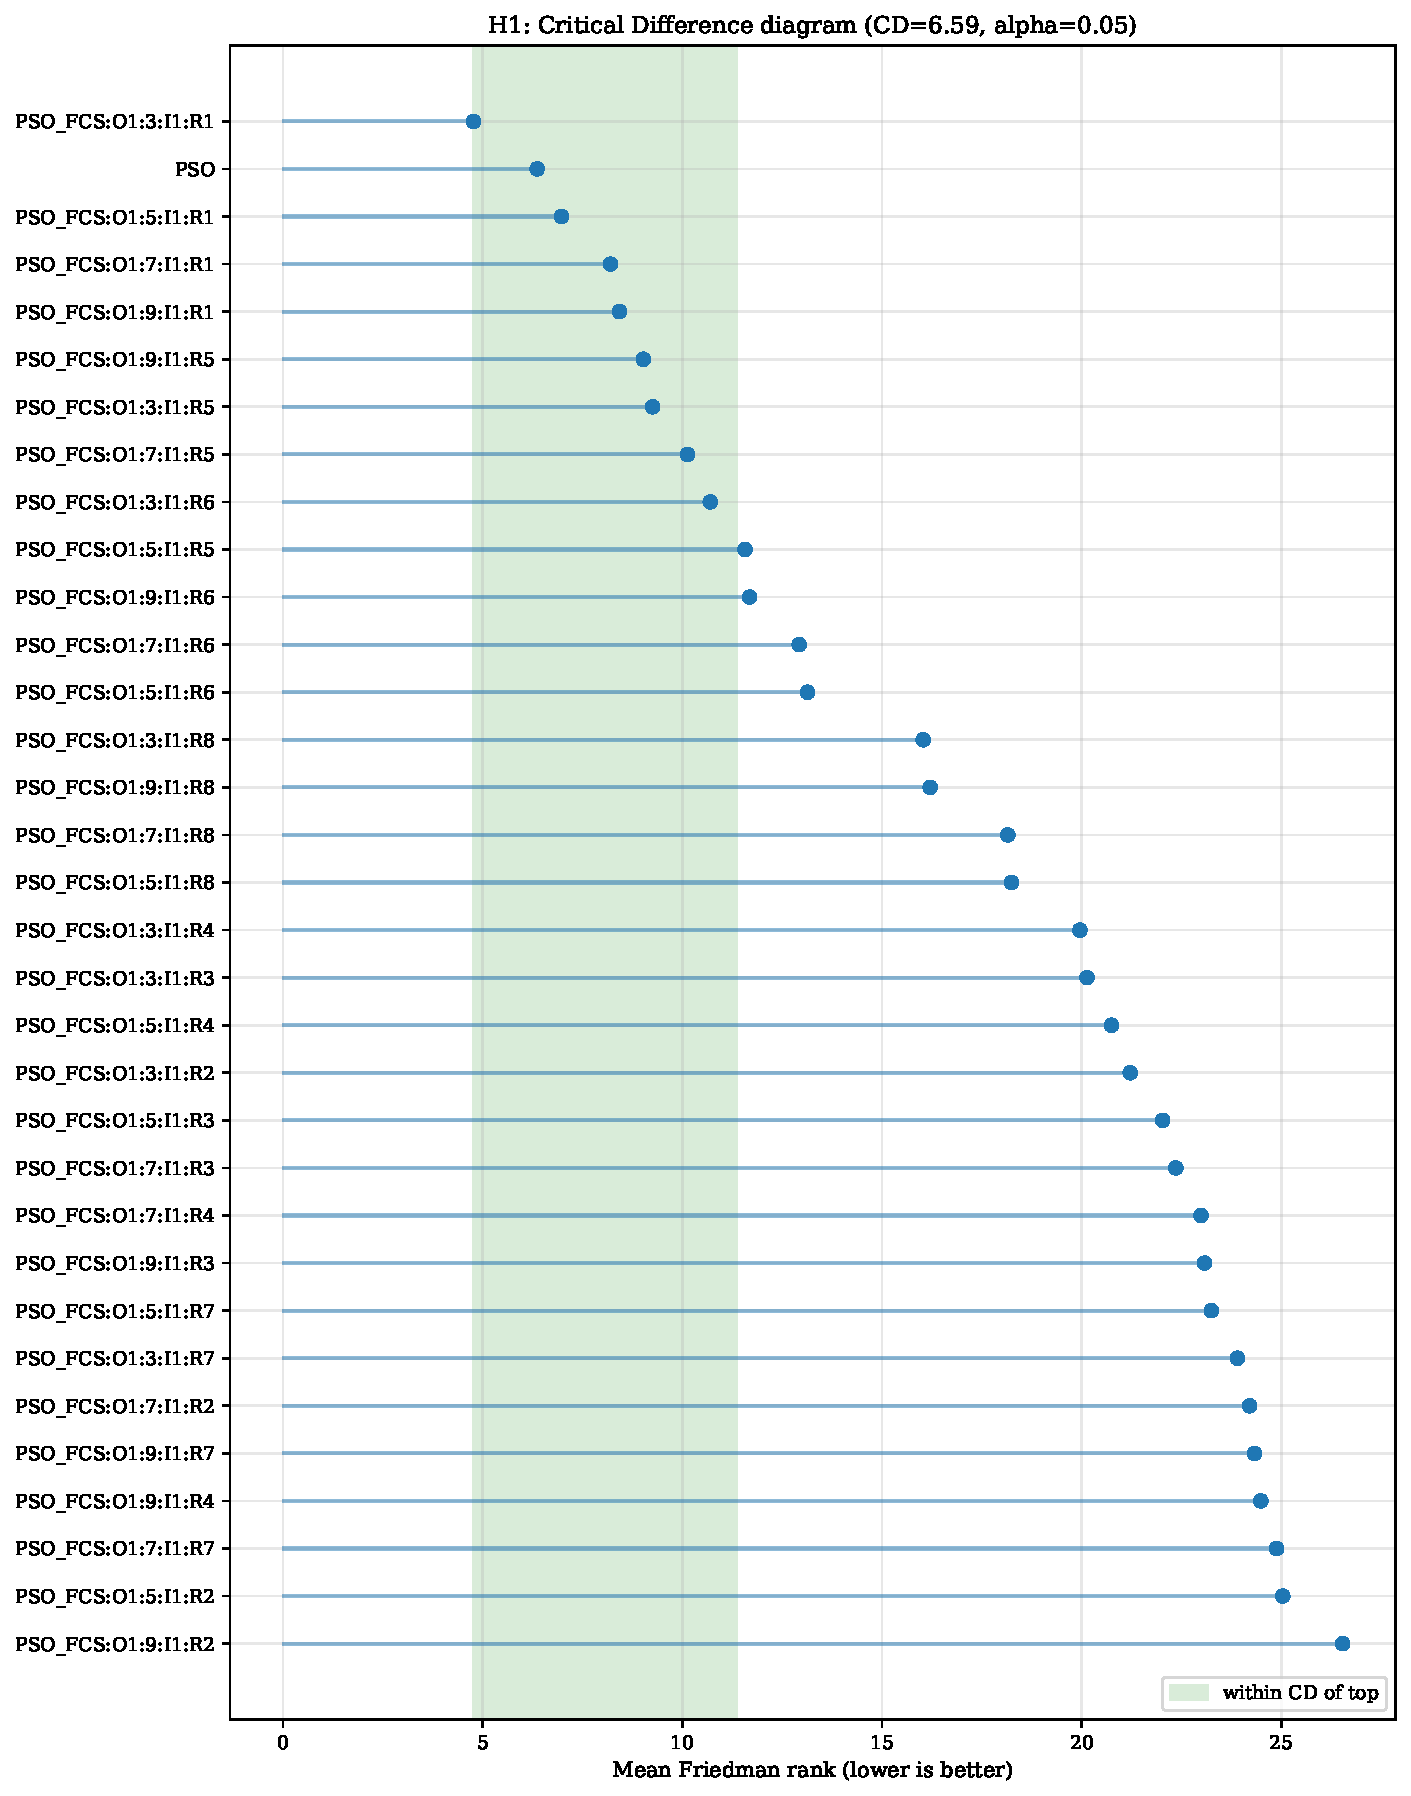
\includegraphics[width=\fulllength,height=0.90\textheight,keepaspectratio]{figures/fig_cd_diagram_h1.pdf}
  \end{adjustwidth}
  \caption{Critical-difference diagram of 33 configurations over 62 instances (Friedman/Nemenyi, $\alpha=0.05$). Lower mean rank is better; shading marks configurations within CD $=6.59$ of the leader. PSO is bold.}
  \label{fig:fig_cd_diagram_h1}
\end{figure}

\subsection{Function-level performance}
\label{subsec:results_function}

The aggregated ranking of Section~\ref{subsec:results_global} hides where each configuration actually wins. Table~\ref{tab:function_level} therefore reports, for every benchmark function, the fuzzy configuration that wins the largest number of its instances, the per-instance rank of that configuration and of the baseline, and the Bonferroni-significant outcomes for the selected configuration. Ranks are computed within each instance over the 33 algorithmic configurations using the median normalized gap, so rank~1 denotes the best configuration on that instance. Configurations are named \texttt{FCS-$n$-R$k$}, where $n$ is the number of linguistic labels and $k$ the rule-base pattern; the input and output partition families are I1 and O1 for every configuration and are therefore omitted from the label.

\afterpage{\startlandscape
\begin{table}[H]
\centering
\small
\caption{Function-level summary of the FCS configuration with the most per-instance rank wins, its ranks, Bonferroni-significant outcomes, effect size, and unpaired runtime overhead.}
\label{tab:function_level}
\setlength{\tabcolsep}{3pt}
\begin{tabular*}{\textwidth}{@{\extracolsep{\fill}}l p{2.8cm} p{1.9cm} p{2.1cm} c c c c c c}
\toprule
\textbf{Function} & \textbf{Landscape} & \textbf{Dimensions} & \textbf{Best FCS} & \textbf{PSO rank} & \textbf{FCS rank} & \textbf{Rank wins} & \textbf{Bonferroni wins} & \boldmath$A_{12}$ & \textbf{Overhead (\%)} \\
\midrule
F1 & Unimodal & 10, 30, 50, 100 & \texttt{FCS-3-R1} & 3.0 & 1.0 & 4/4 & 3/4 & 0.96 & 31.8 \\
F2 & Unimodal & 10, 30, 50, 100 & \texttt{FCS-3-R1} & 2.0 & 1.0 & 4/4 & 4/4 & 0.98 & 34.1 \\
F3 & Unimodal & 10, 30, 50, 100 & \texttt{FCS-5-R5} & 11.0 & 1.0 & 4/4 & 1/4 & 0.74 & 14.6 \\
F4 & Unimodal & 10, 30, 50, 100 & \texttt{FCS-9-R5} & 4.0 & 1.0 & 3/4 & 1/4 & 0.56 & 26.2 \\
F5 & Unimodal & 10, 30, 50, 100 & \texttt{FCS-3-R1} & 3.0 & 1.0 & 4/4 & 0/4 & 0.64 & 29.6 \\
F6 & Unimodal & 10, 30, 50, 100 & \texttt{FCS-3-R1} & 2.0 & 1.0 & 4/4 & 4/4 & 0.95 & 33.9 \\
F7 & Unimodal & 10, 30, 50, 100 & \texttt{FCS-5-R1} & 3.0 & 1.0 & 3/4 & 0/4 & 0.54 & 28.7 \\
\midrule
F8 & Scalable multimodal & 10, 30, 50, 100 & \texttt{FCS-9-R8} & 3.5 & 1.5 & 2/4 & 0/4 & 0.54 & 27.1 \\
F9 & Scalable multimodal & 10, 30, 50, 100 & \texttt{FCS-5-R2} & 9.0 & 1.0 & 4/4 & 0/4 & 0.60 & 25.4 \\
F10 & Scalable multimodal & 10, 30, 50, 100 & \texttt{FCS-3-R1} & 3.5 & 1.0 & 3/4 & 1/4 & 0.77 & 26.9 \\
F11 & Scalable multimodal & 10, 30, 50, 100 & \texttt{FCS-3-R1} & 4.0 & 1.0 & 4/4 & 2/4 & 0.75 & 30.7 \\
F12 & Scalable multimodal & 10, 30, 50, 100 & \texttt{FCS-3-R1} & 2.0 & 1.0 & 3/4 & 0/4 & 0.72 & 25.4 \\
F13 & Scalable multimodal & 10, 30, 50, 100 & \texttt{FCS-3-R1} & 3.0 & 1.0 & 4/4 & 0/4 & 0.74 & 28.7 \\
\midrule
F14 & Fixed-dimensional & 2 & \texttt{FCS-3-R1} & 27.0 & 3.0 & 1/1 & 0/1 & 0.58 & -5.0 \\
F15 & Fixed-dimensional & 4 & \texttt{FCS-3-R1} & 11.0 & 1.0 & 1/1 & 0/1 & 0.75 & 86.9 \\
F16 & Fixed-dimensional & 2 & -- & 17.0 & 17.0 & 0/1 & 0/1 & 0.56 & -- \\
F17 & Fixed-dimensional & 2 & -- & 17.0 & 17.0 & 0/1 & 0/1 & 0.50 & -- \\
F18 & Fixed-dimensional & 2 & \texttt{FCS-3-R1} & 15.0 & 15.0 & 0/1 & 0/1 & 0.45 & 161.5 \\
F19 & Fixed-dimensional & 3 & -- & 17.0 & 17.0 & 0/1 & 0/1 & 0.56 & -- \\
F20 & Fixed-dimensional & 6 & \texttt{FCS-3-R1} & 14.0 & 14.0 & 0/1 & 0/1 & 0.55 & 53.2 \\
F21 & Fixed-dimensional & 4 & \texttt{FCS-7-R1} & 24.0 & 1.0 & 1/1 & 0/1 & 0.61 & 17.8 \\
F22 & Fixed-dimensional & 4 & \texttt{FCS-3-R6} & 20.0 & 1.0 & 1/1 & 0/1 & 0.57 & 14.6 \\
F23 & Fixed-dimensional & 4 & \texttt{FCS-5-R6} & 1.0 & 2.0 & 0/1 & 0/1 & 0.34 & 8.2 \\
\bottomrule
\end{tabular*}
\noindent\footnotesize
Ranks are medians of per-instance ranks on median normalized gap (lower is better). Rank wins count instances where the selected FCS has a lower rank than PSO. Bonferroni wins use independent-sample Mann--Whitney tests adjusted over all 1,984 RQ4 comparisons. $A_{12}$ is the median effect size; $A_{12}>0.5$ favours FCS. Overhead is $100(\mathrm{median}(t_{\mathrm{FCS}})/\mathrm{median}(t_{\mathrm{PSO}})-1)$ using independent run samples. A dash marks functions where all FCS configurations share the best median-gap rank.
\end{table}
\finishlandscape
\restoreportraitheight}

Three observations follow from the disaggregated view. First, the best fuzzy configuration outranks the baseline on 50 of the 62 instances. Of these rank wins, 32 have nominal independent-sample $p<0.05$ and 17 remain significant after Bonferroni correction across the RQ4 family. The baseline ranks ahead on 6 instances, and the best FCS and PSO share the minimum rank on the remaining 6. Second, the winning configuration is not unique: 15 distinct FCS configurations record at least one rank-based win over PSO. \texttt{FCS-3-R1} accounts for 30 of the 50 wins, including 28 of the 46 wins in the scalable subset $S_1$; the other wins span all four granularities and six additional rule patterns. The function-level table identifies the best fuzzy candidate even when it does not outrank PSO. Third, the effect size is heterogeneous: the median $A_{12}$ reaches 0.95--0.98 on F1, F2, and F6, but remains near 0.54 on F7 and F8 and on most fixed-dimensional functions.

The fixed-dimensional subset behaves differently from the scalable one. On F16 and F17, normalized gap is zero in all 31 runs for all 33 configurations. On F19, 990 of 1023 run-level gaps are zero; although 33 runs have a nonzero gap, every configuration has a zero median gap. The 33 configurations therefore share mean rank 17 on these functions, and no unique median-gap winner is identified. For F16, the independent-sample test on raw final fitness is nominally significant ($p=0.0419$), but its Bonferroni-adjusted $p$ is 1.000; $A_{12}=0.56$ and all normalized gaps are zero, so the test does not establish a normalized-gap advantage. On F14, F15, F21, and F22 the baseline falls to ranks 11--27 while a fuzzy configuration takes the first position. On F23, the ordering reverses: PSO takes the first position and the best fuzzy configuration, \texttt{FCS-5-R6}, ranks second with $A_{12}=0.34$, favouring PSO. The independent-sample $p=0.0234$ is nominally significant but does not survive Bonferroni correction. This subset therefore includes both large rank differences favouring fuzzy control and a function on which PSO ranks first; it does not support a universally dominant configuration.

Figure~\ref{fig:fig_function_heatmap} in Appendix~\ref{app:instance_results} shows the complete rank matrix: columns are ordered by mean rank, PSO is bracketed, and the S1/S2 boundary is marked. It shows predominantly better FCS ranks across the scalable subset and more varied outcomes across fixed-dimensional instances, complementing Table~\ref{tab:function_level}.

\subsection{Problem-class dependence}
\label{subsec:results_class}

Across the evaluated configurations, performance rankings show greater variation among rule-base patterns (R1--R8) than among linguistic granularities ($n \in \{3,5,7,9\}$). Figure~\ref{fig:fig_rule_class_heatmap} presents, for each configuration and landscape class, the mean across instances of the instance-level median normalized gap (smaller is better). The classes are unimodal functions (F1--F7), scalable multimodal functions (F8--F13), and fixed-dimensional multimodal functions (F14--F23); each configuration appears once as a row.

\begin{figure}[!htbp]
  \centering
  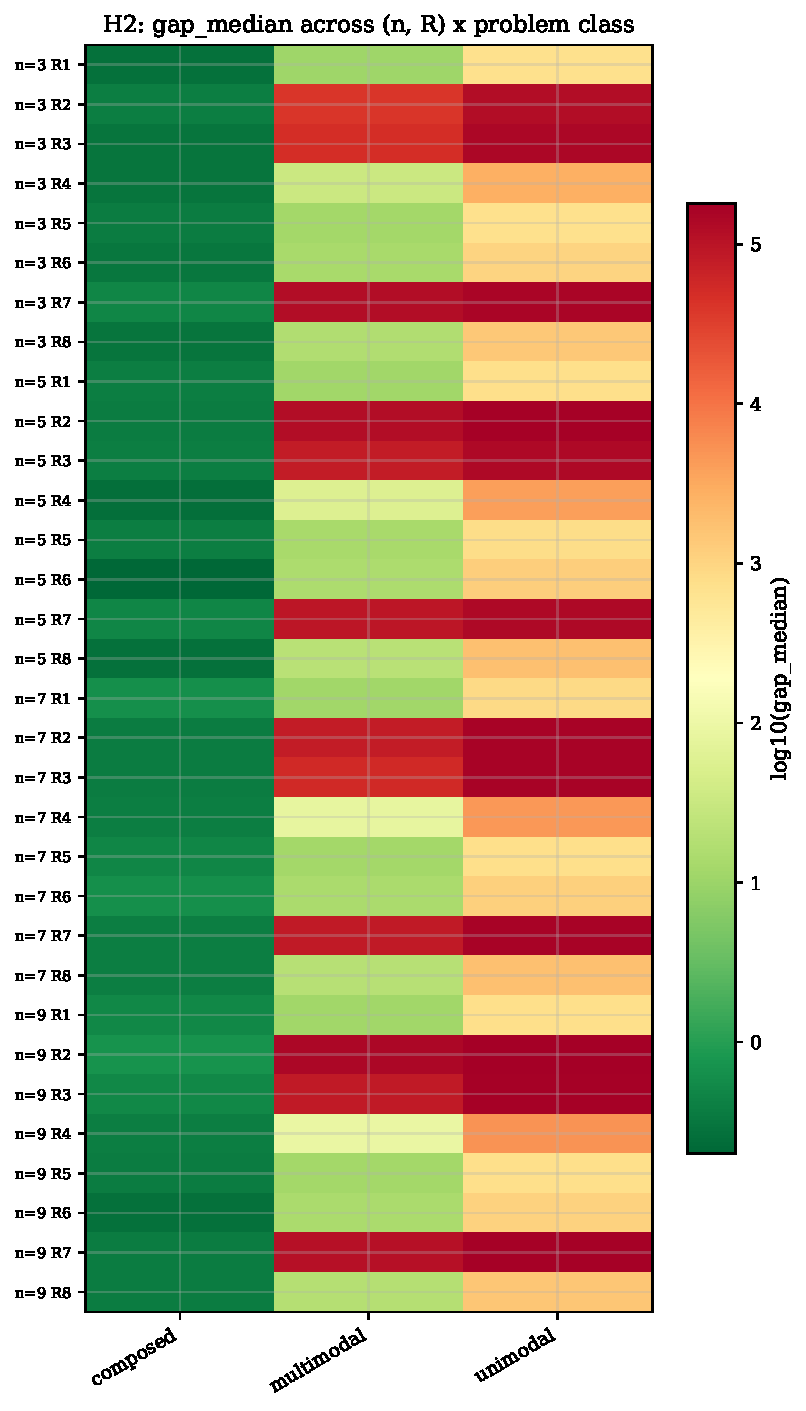
\includegraphics[width=0.65\linewidth]{figures/fig_rule_class_heatmap.pdf}
  \caption{Mean instance-level median normalized gap for the 32 FCS configurations by landscape class. Colour shows $\log_{10}$ mean gap with a $10^{-12}$ display floor; lower values indicate better performance.}
  \label{fig:fig_rule_class_heatmap}
\end{figure}

Two complementary partitions of the benchmark are used. For landscape effects, functions are grouped as unimodal (F1--F7), scalable multimodal (F8--F13), and fixed-dimensional multimodal (F14--F23). For the transferability analysis, the benchmark is split into the scalable subset $S_1$ (F1--F13, evaluated at four dimensions each) and the fixed-dimensional subset $S_2$ (F14--F23); this split is by dimensional regime, not by modality.

Table~\ref{tab:class_summary} summarizes the class-level rankings. The leading configuration differs across the evaluated groups: \texttt{FCS-3-R5} leads on unimodal functions, \texttt{FCS-3-R1} on scalable multimodal functions, and \texttt{FCS-5-R6} on fixed-dimensional functions. \texttt{FCS-3-R1} remains relatively competitive, ranking 2nd, 1st, and 3rd, respectively. These descriptive results do not isolate causal effects of modality or dimensionality, nor establish a universally optimal configuration for any group.

\begin{table}[!htbp]
\centering
\small
\caption{Positions of the 33 configurations by mean instance-level median normalized gap within each benchmark group (lower is better). For each configuration--instance pair, the median normalized gap over 31 runs was first computed; these medians were then averaged within the group. Positions use minimum ranks for ties and are not Friedman mean ranks.}
\label{tab:class_summary}
\setlength{\tabcolsep}{3pt}
\begin{tabularx}{\textwidth}{@{}>{\raggedright\arraybackslash}Xcc>{\raggedright\arraybackslash}p{2.7cm}cc@{}}
\toprule
\textbf{Benchmark group} & \textbf{Functions} & \textbf{Instances} & 
\textbf{Leading configuration} & \textbf{PSO position} & \textbf{FCS-3-R1 position} \\
\midrule
Unimodal (F1--F7) & 7 & 28 & FCS-3-R5 & 8/33 & 2/33 \\
Scalable multimodal (F8--F13) & 6 & 24 & FCS-3-R1 & 2/33 & 1/33 \\
Fixed-dimensional (F14--F23) & 10 & 10 & FCS-5-R6 & 25/33 & 3/33 \\
\bottomrule
\end{tabularx}
\end{table}


As a descriptive sensitivity check, configurations were also ranked by median normalized gap within each instance and these ranks were averaged by benchmark group. Under mean within-instance ranks, FCS-3-R1 leads the unimodal group (with PSO 2nd and FCS-3-R1 1st), remains the scalable multimodal leader (PSO 2nd and FCS-3-R1 1st), and FCS-5-R6 remains the fixed-dimensional leader (PSO 17th and FCS-3-R1 2nd). The unimodal leader therefore changes from FCS-3-R5 under mean instance-level median gap to FCS-3-R1 under mean within-instance rank. The gap mean preserves magnitude differences among instances, whereas the rank mean summarizes relative ordering with equal instance weight; neither aggregation is universally superior.

Table~\ref{tab:kendall_class} reports Kendall $\tau$ between the configuration rankings induced by each pair of landscape classes. The two scalable classes show strong observed rank concordance ($\tau=0.867$ between unimodal and scalable multimodal); the fixed-dimensional class shows weak observed concordance with them ($\tau=0.080$ and $\tau=0.083$). These coefficients describe the evaluated classes and do not establish independence or a general transferability result.

\begin{table}[h]
\centering
\caption{Kendall's tau between rankings induced by the three problem classes (higher = more agreement).}
\label{tab:kendall_class}
\begin{tabular}{llll}
\toprule
class & composed & multimodal & unimodal \\
\midrule
composed & 1.000 & 0.080 & 0.083 \\
multimodal & 0.080 & 1.000 & 0.867 \\
unimodal & 0.083 & 0.867 & 1.000 \\
\bottomrule
\end{tabular}
\end{table}


Rank concordance between $S_1$ and $S_2$ is weak ($\tau=0.095$, $p=0.451$); this non-significant result does not establish independence. \texttt{FCS-3-R5} has the lowest mean normalized gap on $S_1$ and ranks 11th on $S_2$, whereas \texttt{FCS-5-R6} leads on $S_2$ and ranks 13th on $S_1$. These rankings describe only the evaluated subsets.

Figure~\ref{fig:fig_pareto_s1_s2} plots the configuration ranks in the $(S_1,S_2)$ space and highlights the non-dominated frontier. No configuration achieves the best rank on both subsets: the frontier includes the two subset specialists and \texttt{FCS-3-R1}, which ranks second on S1 and third on S2 and offers the closest observed compromise. This dispersion is the aggregated counterpart of the per-instance heterogeneity reported in Section~\ref{subsec:results_function}.


\begin{figure}[!h]
  \centering
  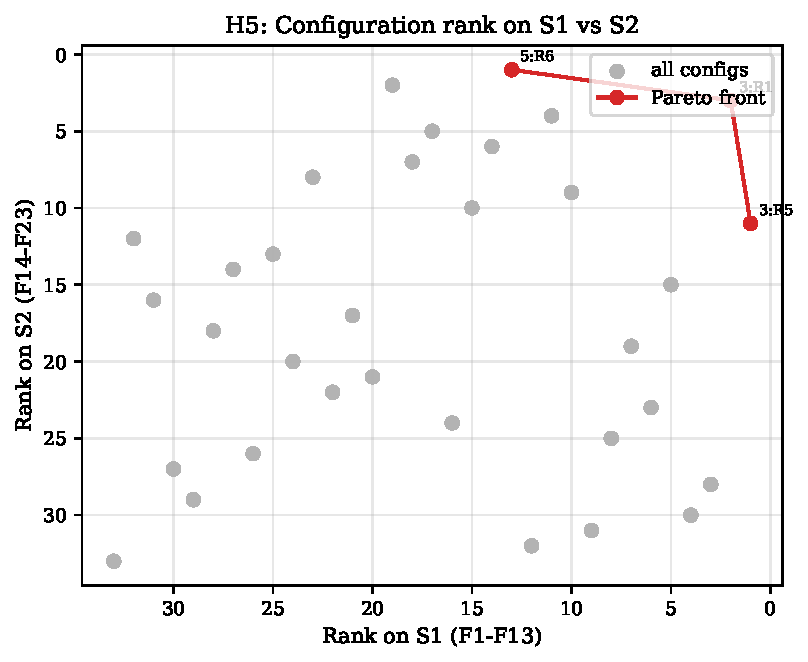
\includegraphics[width=0.85\linewidth]{figures/fig_pareto_s1_s2.pdf}
  \caption{Configuration ranks on S1 versus S2, computed from per-instance median normalized gap; better ranks lie toward the upper right. The red line marks the non-dominated frontier and the star denotes PSO.}
  \label{fig:fig_pareto_s1_s2}
\end{figure}

\subsection{Effect of rule-base structure}
\label{subsec:results_rules}

Sections~\ref{subsec:results_global}--\ref{subsec:results_class} establish that rule-table patterns separate the configurations more sharply than the number of labels, but do not by themselves attribute this ranking to independent input effects. As defined in Section~\ref{subsec:formal_rules}, R1--R8 combine two nominal consequent axes: progress direction (decreasing, neutral, or increasing) and diversity reaction (following, neutral, or compensating). Table~\ref{tab:rule_semantic_grid} places the patterns on those axes with their mean Friedman rank across the four granularities. A neutral consequent axis does not guarantee that the corresponding input is absent from the effective Mamdani surface.

\begin{table}[H]
\centering
\small
\caption{Mean Friedman ranks by nominal progress direction and diversity consequent, averaged over four granularities. A neutral consequent does not remove an antecedent from Mamdani inference.}
\label{tab:rule_semantic_grid}
\begin{tabular}{lccc}
\toprule
 & \textbf{Diversity-following} & \textbf{Diversity-neutral} & \textbf{Diversity-compensating} \\
\midrule
\textbf{Progress decreasing} & R5 (10.0) & R1 (7.1) & R6 (12.1) \\
\textbf{Progress neutral} & R3 (21.9) & -- & R4 (22.0) \\
\textbf{Progress increasing} & R7 (24.1) & R2 (24.3) & R8 (17.2) \\
\bottomrule
\end{tabular}
\end{table}


The grid is ordered almost entirely by rows. The three patterns with a decreasing progress effect occupy the best mean ranks (R1 = 7.1, R5 = 10.0, R6 = 12.1), the two progress-neutral patterns sit in the lower half (R3 = 21.9, R4 = 22.0), and two of the three patterns with an increasing progress effect close the ranking (R7 = 24.1, R2 = 24.3). Column position accounts for a much smaller spread: within the decreasing row the three patterns differ by 5.0 ranks, whereas the difference between the best and the worst row exceeds 17 ranks.

To compare rule-pattern contrasts, the 31 run-level outcomes for each pattern are treated as independent samples at equal granularity and on the same instance. The two-sided Mann--Whitney tests are adjusted with Holm's procedure across all 1,984 contrasts. Mirror pairs invert every non-neutral consequent axis and, by Proposition~\ref{prop:mirror}, reflect the control surface about the midpoint of $[w_{\min},w_{\max}]$. Single-axis pairs change one nominal consequent axis while holding the other fixed. These are descriptive comparisons of rule tables; they do not imply orthogonal effective-input effects under min--max inference. Table~\ref{tab:rule_pairs} reports both pair families.

\begin{table}[!htbp]
\centering
\small
\caption{Independent-sample comparisons of rule-pattern pairs at equal granularity and instance (248 tests per pair). Holm adjustment is applied once across the complete family of 1,984 comparisons.}
\label{tab:rule_pairs}
\begin{adjustwidth}{-\extralength}{0cm}
\setlength{\tabcolsep}{4pt}
\renewcommand{\arraystretch}{1.15}
\renewcommand{\tabularxcolumn}[1]{m{#1}}
\begin{tabularx}{\fulllength}{@{}l>{\raggedright\arraybackslash}X c c c c l@{}}
\toprule
\textbf{Pair} & \textbf{Axis changed} & \textbf{Nominal W/NS/L} & \textbf{Holm W/NS/L} & \textbf{Dominant} & \boldmath$A_{12}$ & \textbf{Strongest in} \\
\midrule
\multicolumn{7}{l}{\emph{Mirror pairs}} \\
R1 vs R2 & progress direction & 192/56/0 & 175/73/0 & \textbf{R1} & 0.99 & Unimodal \\
R3 vs R4 & diversity reaction & 118/59/71 & 104/98/46 & \textbf{R4} & 0.41 & Scalable multimodal \\
R5 vs R8 & progress direction + diversity reaction & 173/73/2 & 142/106/0 & \textbf{R5} & 0.91 & Unimodal \\
R6 vs R7 & progress direction + diversity reaction & 173/57/18 & 152/91/5 & \textbf{R6} & 0.95 & Scalable multimodal \\
\midrule
\multicolumn{7}{l}{\emph{Single-axis pairs}} \\
R5 vs R7 & progress direction & 172/75/1 & 152/96/0 & \textbf{R5} & 0.96 & Scalable multimodal \\
R6 vs R8 & progress direction & 176/65/7 & 156/92/0 & \textbf{R6} & 0.92 & Unimodal \\
R5 vs R6 & diversity reaction & 132/81/35 & 99/130/19 & \textbf{R5} & 0.66 & Unimodal \\
R7 vs R8 & diversity reaction & 154/68/26 & 137/98/13 & \textbf{R8} & 0.09 & Scalable multimodal \\
\bottomrule
\end{tabularx}
\noindent\footnotesize
W/NS/L denotes significant wins for the dominant pattern, non-significant comparisons, and significant losses. Nominal counts use $p<0.05$; Holm counts use adjusted $p<0.05$ across all 1,984 tests. $A_{12}$ is the median effect for the first pattern; values above 0.5 favour it. These contrasts compare implemented rule tables and do not isolate causal input effects.
\end{adjustwidth}
\end{table}


After Holm correction across the full Table 11 family, the decreasing-progress pattern has more significant wins than losses in each matched contrast with its increasing-progress counterpart: R1 over R2, 175/73/0 (wins/non-significant/losses); R5 over R7, 152/96/0; and R6 over R8, 156/92/0. Their median $A_{12}$ values are 0.99, 0.96, and 0.92, respectively. These are empirical differences among the tested rule tables, not evidence that the effective controller responds only to progress.

Among patterns with different diversity consequents, the Holm-adjusted independent-sample comparisons also vary with the nominal progress direction. For decreasing progress, R5 has 99 significant wins and 19 losses against R6, with 130 non-significant comparisons ($A_{12}=0.66$). For increasing progress, R8 has 137 wins and 13 losses against R7, with 98 non-significant comparisons ($A_{12}=0.09$ in favour of R8). For the nominally progress-neutral pattern, R4 has 104 wins and 46 losses against R3, with 98 non-significant comparisons; their aggregate mean ranks remain close (22.0 and 21.9). These comparisons describe the tested rule tables and do not establish a general benefit of diversity feedback.

Both effects are also visible in the mirror pairs, which reverse the pattern as a whole. R1 dominates R2 and R5 dominates R8 most clearly on the unimodal class, whereas R6 dominates R7 most clearly on the scalable multimodal class, which is consistent with the landscape dependence reported in Section~\ref{subsec:results_class}.

These results explain the composition of the leading group of Section~\ref{subsec:results_global}. Every configuration inside the critical-difference band uses a decreasing-progress consequent pattern: the four R1 variants, three R5 variants, and one R6 variant. No pattern with a nominally neutral or increasing progress consequent enters the band, and R2, R3, R4, R7, and R8 remain outside it at every granularity. The single exception to the row ordering, R8 at rank 17.2 ahead of the nominally progress-neutral R3 and R4, combines an increasing-progress consequent with the compensating diversity consequent favoured by the Holm-adjusted R7--R8 contrast. Overall, rankings align most strongly with nominal progress-consequent direction, while independent-sample differences across diversity-consequent patterns depend on that direction. Since a neutral consequent axis does not remove the input from min--max firing, these comparisons are not independent causal effects of the two inputs.

\subsection{Effect of linguistic granularity}
\label{subsec:results_granularity}

Granularity cannot be read in isolation from the rule-base pattern, because $n$ fixes the resolution at which a pattern is expressed and simultaneously raises the number of consequents from $n^2 = 9$ at $n=3$ to $n^2 = 81$ at $n=9$. Table~\ref{tab:granularity_by_rule} therefore reports the mean Friedman rank of every pattern at each granularity, together with the granularity that minimizes it and the spread between its best and worst rank.

\begin{table}[H]
\centering
\small
\caption{Mean Friedman rank of each rule-base pattern at each granularity (lower is better). Spread is the maximum minus minimum across $n$; the 2.5-rank stability threshold is descriptive, not an equivalence test.}
\label{tab:granularity_by_rule}
\setlength{\tabcolsep}{3.5pt}
\begin{tabular}{lcccccccl}
\toprule
\textbf{Pattern} & \textbf{Progress} & \boldmath$n=3$ & \boldmath$n=5$ & \boldmath$n=7$ & \boldmath$n=9$ & \textbf{Best} \boldmath$n$ & \textbf{Spread} & \textbf{Trend} \\
\midrule
R1 & dec. & 4.8 & 7.0 & 8.2 & 8.4 & 3 & 3.7 & degradation \\
R2 & incr. & 21.2 & 25.0 & 24.3 & 26.5 & 3 & 5.3 & degrad. (non-monot.) \\
R3 & neutral & 20.1 & 22.0 & 22.4 & 23.1 & 3 & 2.9 & degradation \\
R4 & neutral & 20.0 & 20.8 & 23.0 & 24.5 & 3 & 4.5 & degradation \\
R5 & dec. & 9.2 & 11.6 & 10.1 & 9.0 & 9 & 2.5 & non-monotonic \\
R6 & dec. & 10.7 & 13.1 & 12.9 & 11.7 & 3 & 2.4 & stable \\
R7 & incr. & 23.9 & 23.2 & 24.9 & 24.3 & 5 & 1.6 & stable \\
R8 & incr. & 16.0 & 18.2 & 18.1 & 16.2 & 3 & 2.2 & stable \\
\bottomrule
\end{tabular}
\end{table}


Six of the eight patterns attain their best rank at $n=3$; the exceptions are R5, which is marginally better at $n=9$ (9.02 against 9.25), and R7, which is marginally better at $n=5$ within a spread of 1.6 ranks. The response to $n$ is pattern-dependent. R1's mean rank worsens monotonically from 4.77 at $n=3$ to 8.43 at $n=9$, an increase of 3.65 positions, but this is not the largest change across patterns: R2 increases by 5.33 positions (spread 5.3) and R4 by 4.53 (spread 4.5). Here, spread is the maximum minus minimum mean rank over the four granularities. R6, R7, and R8 show comparatively small observed spreads of 2.4, 1.6, and 2.2 positions, respectively. The table's 2.5-rank stability threshold is descriptive; it does not establish equivalence or absence of a granularity effect.

The aggregate view agrees. Averaged over the eight patterns, the mean rank worsens from 15.74 at $n=3$ to 17.62 at $n=5$ and then remains near 17.99 and 17.97 for $n=7$ and $n=9$; the best rank achievable at each granularity degrades monotonically from 4.77 to 6.97, 8.20, and 8.43. The distribution of the normalized gap, shown in Figure~\ref{fig:fig_boxplot_gap_by_n}, follows the same shape: the median of $\log_{10}$ gap rises from 0.02 at $n=3$ to 0.22 at $n=5$ and then settles at 0.21 and 0.19, while the interquartile range contracts from 3.50 to 3.19 and remains at 3.24 and 3.27. The observed gap worsens from three to five labels and then changes little through $n=9$.

\begin{figure}[!h]
  \centering
  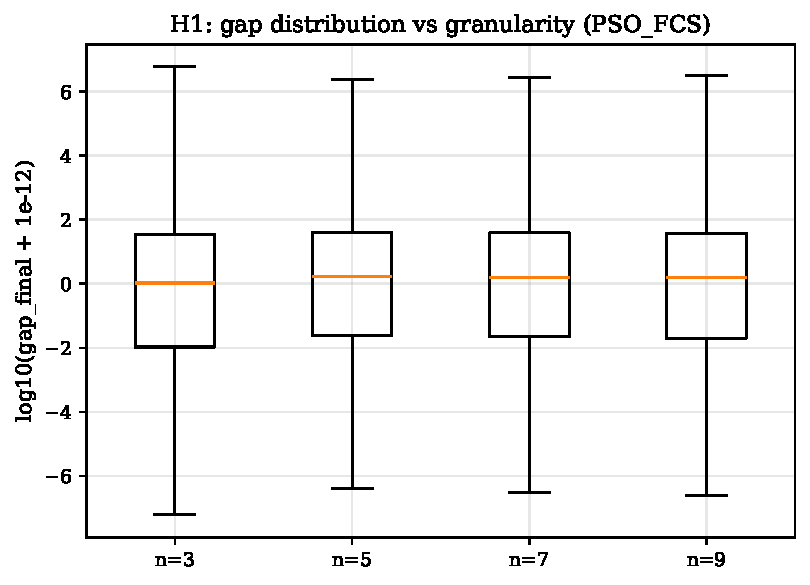
\includegraphics[width=0.85\linewidth]{figures/fig_boxplot_gap_by_n.pdf}
  \caption{Boxplots of run-level final normalized gap, transformed as $\log_{10}(\max(\mathrm{gap},10^{-12})+10^{-12})$ and pooled over 62 instances and eight FCS patterns at each granularity. Outliers are omitted.}
  \label{fig:fig_boxplot_gap_by_n}
\end{figure}

Figure~\ref{fig:fig_granularity_effect} descriptively traces each rule-base pattern across linguistic granularities. Across $n=3$, $5$, $7$, and $9$, the progress-decreasing family remains ahead of the other two nominal consequent-direction families, with R1, R5, and R6 occupying the first three positions at every evaluated granularity. Kendall's $\tau$ between the orderings of the eight patterns at different granularities ranges from 0.79 to 0.93, with the minimum observed between the most distant pair, $n=3$ and $n=9$. Changes in granularity mainly shift the patterns vertically without altering the identity of the leading family; the observed exchanges of position occur within the lower-ranked group outside the critical-difference band, where R2, R3, R4, and R7 interchange positions. These benchmark-wide profiles describe relative ranks and should be distinguished from performance-gap dispersion or a formal interaction effect.

\begin{figure}[!h]
  \centering
  \includegraphics[width=\textwidth]{figures/fig_granularity_effect.pdf}
  \caption{Benchmark-wide summaries over the 62 function--dimension instances. Left: mean Friedman rank by rule-base pattern and linguistic granularity, where better (lower) ranks appear toward the top; colour and line style indicate the nominal direction of the progress consequents. Right: standard deviation across the eight pattern-specific mean ranks for each granularity.}
  \label{fig:fig_granularity_effect}
\end{figure}

In the benchmark-wide summary, the standard deviation across the eight mean Friedman ranks is 6.778, 6.397, 6.707, and 7.524 for $n=3,5,7,9$. The standard deviation across the eight pooled median normalized gaps is 3.994, 4.460, 4.470, and 4.635; these gap medians pool 1,922 run-level observations per pattern and granularity. The median of the function-level rank spreads across the 23 functions is 8.884, 8.366, 8.715, and 9.374; the corresponding log-gap spreads are 0.912, 1.170, 1.173, and 0.901. For ranks, the $S_1$ medians are 8.884, 8.789, 9.128, and 10.194, while the $S_2$ medians are 7.255, 6.556, 6.834, and 5.456. For log-gaps, the $S_1$ medians are 1.359, 1.468, 1.374, and 1.396, and the $S_2$ medians are 0.075, 0.308, 0.263, and 0.070. From $n=3$ to $n=9$, rank spread is lower in 6/23 functions and log-gap spread in 11/23; each measure is non-increasing across all four granularities in 3/23 functions. The observed dispersion therefore does not decrease consistently as linguistic granularity increases. Together with the configuration rankings and pattern-dependent responses reported above, this finding indicates that finer linguistic partitions do not guarantee better optimization performance or more consistent behavior across rule-base patterns. Within the evaluated Mamdani controllers, the organization of the consequent rules remains an important design consideration, rather than linguistic resolution alone. These observations are descriptive and do not establish independent causal effects, statistical equivalence, or a formal granularity-by-rule interaction.


\subsection{Robustness, dimensional scaling, and computational overhead}
\label{subsec:results_robustness}

Section~\ref{subsec:results_function} measured the best fuzzy configuration available on each instance, which is an oracle selection: the winner is allowed to change from one instance to the next. The complementary and stricter question is whether a \emph{single fixed} configuration, chosen once and applied everywhere, beats the baseline across the benchmark. Table~\ref{tab:h4_wilcoxon} reports the ten configurations with the largest number of Bonferroni-significant wins, ordered by corrected wins, nominal wins, and then mean $A_{12}$. Each configuration is compared with PSO on all 62 instances using independent samples and a two-sided Mann--Whitney $U$ test. Because the objective is minimized, the Vargha--Delaney effect size is defined so that $A_{12} > 0.5$ favours the fuzzy configuration and $A_{12} < 0.5$ favours the baseline.

\begin{table}[h]
\centering
\caption{Wilcoxon signed-rank comparison of top-10 PSO\_FCS configurations against classical PSO (paired by run). Columns marked * apply Bonferroni correction over the full 32x62 grid.}
\label{tab:h4_wilcoxon}
\begin{tabular}{llllllllll}
\toprule
Config. & n & R & Wins & Ties & Losses & Wins* & Ties* & Losses* & A12 mean \\
\midrule
PSO\_FCS:O1:3:I1:R1 & 3.000 & R1 & 27 & 33 & 2 & 13 & 49 & 0 & 0.669 \\
PSO\_FCS:O1:7:I1:R5 & 7.000 & R5 & 6 & 28 & 28 & 1 & 43 & 18 & 0.363 \\
PSO\_FCS:O1:9:I1:R5 & 9.000 & R5 & 5 & 31 & 26 & 0 & 47 & 15 & 0.383 \\
PSO\_FCS:O1:5:I1:R5 & 5.000 & R5 & 5 & 24 & 33 & 0 & 38 & 24 & 0.304 \\
PSO\_FCS:O1:5:I1:R1 & 5.000 & R1 & 4 & 51 & 7 & 0 & 62 & 0 & 0.463 \\
PSO\_FCS:O1:3:I1:R5 & 3.000 & R5 & 4 & 27 & 31 & 0 & 48 & 14 & 0.358 \\
PSO\_FCS:O1:9:I1:R1 & 9.000 & R1 & 2 & 53 & 7 & 0 & 62 & 0 & 0.444 \\
PSO\_FCS:O1:7:I1:R7 & 7.000 & R7 & 2 & 14 & 46 & 0 & 23 & 39 & 0.173 \\
PSO\_FCS:O1:7:I1:R1 & 7.000 & R1 & 1 & 55 & 6 & 0 & 62 & 0 & 0.447 \\
PSO\_FCS:O1:3:I1:R6 & 3.000 & R6 & 1 & 23 & 38 & 0 & 35 & 27 & 0.225 \\
\bottomrule
\end{tabular}
\end{table}


The leading fixed configuration, \texttt{FCS-3-R1}, records nominal W/NS/L = 30/30/2 and mean $A_{12}=0.67$; Bonferroni adjustment leaves 16/46/0. The other R1 granularities have 62 non-significant results each after correction, despite nominal non-significant counts of 54, 56, and 53. This is not an equivalence result. Several R5 and R7 variants have more adjusted losses than wins, with mean $A_{12}$ favouring PSO. The 50/62 instance-specific rank wins remain an oracle summary, not a deployable policy.

Figure~\ref{fig:fig_h4_independent_outcomes} presents the nominal comparison outcomes, while Table~\ref{tab:h4_wilcoxon} reports Bonferroni-adjusted results and effect sizes. The supplementary mean--dispersion plots illustrate performance variability across representative instances, with lower values on both axes indicating better outcomes. Selected FCS configurations show favourable outcomes on F1 and F14, whereas classical PSO achieves a lower mean normalized gap on F23.


Dimensional robustness was assessed on the scalable subset $S_1$ (F1--F13) at dimensions 10, 30, 50, and 100. For each configuration and function, the median normalized gap at dimension $d$ was transformed as $y=\log_{10}(\max(\text{gap}_{\mathrm{median}},10^{-12})+10^{-12})$, and the log--log slope $b$ in $y=a+b\log_{10}(d)$ was averaged over the thirteen functions. Table~\ref{tab:scaling_slopes} lists the five configurations with the gentlest and the five with the steepest slopes.

\begin{table}[h]
\centering
\caption{Log-log slope of median gap vs dimension for the five best- and five worst-scaling configurations.}
\label{tab:scaling_slopes}
\begin{tabular}{lllllll}
\toprule
Status & Config. & n & R & Mean slope & Median slope & Mean R\textasciicircum{}2 \\
\midrule
best-scaling & PSO\_FCS:O1:5:I1:R4 & 5.000 & R4 & 2.390 & 2.328 & 0.977 \\
best-scaling & PSO\_FCS:O1:9:I1:R4 & 9.000 & R4 & 2.238 & 2.385 & 0.985 \\
best-scaling & PSO\_FCS:O1:3:I1:R4 & 3.000 & R4 & 2.565 & 2.432 & 0.977 \\
best-scaling & PSO\_FCS:O1:7:I1:R4 & 7.000 & R4 & 2.348 & 2.435 & 0.982 \\
best-scaling & PSO\_FCS:O1:9:I1:R7 & 9.000 & R7 & 3.237 & 2.590 & 0.867 \\
worst-scaling & PSO\_FCS:O1:5:I1:R1 & 5.000 & R1 & 8.321 & 12.447 & 0.894 \\
worst-scaling & PSO\_FCS:O1:7:I1:R5 & 7.000 & R5 & 8.738 & 12.488 & 0.865 \\
worst-scaling & PSO\_FCS:O1:5:I1:R5 & 5.000 & R5 & 8.815 & 12.511 & 0.853 \\
worst-scaling & PSO\_FCS:O1:3:I1:R5 & 3.000 & R5 & 8.527 & 12.651 & 0.881 \\
worst-scaling & PSO\_FCS:O1:9:I1:R5 & 9.000 & R5 & 8.789 & 12.723 & 0.873 \\
\bottomrule
\end{tabular}
\end{table}


The four R4 variants occupy the five gentlest slopes, with mean values between 2.24 and 2.56 and $R^2$ above 0.97, while the steepest slopes belong to the R1 and R5 variants, with mean values near 8.3--8.8 and median values above 12.1. A gentle slope, however, is not evidence of better behaviour at large dimension, because the fit measures relative degradation from each configuration's own starting point. \texttt{FCS-5-R4} begins at a median gap of $6.7 \times 10^{-1}$ at $d=10$, twelve orders of magnitude above the $4.5 \times 10^{-13}$ of \texttt{FCS-3-R1}, and it remains worse at $d=100$ ($2.8 \times 10^{1}$ against $7.3$). Its flat slope reflects a configuration that is already poor at low dimension and therefore has little room left to degrade. Slope should accordingly be read as a descriptor of the degradation profile, not as a criterion for selecting a configuration for large-scale problems.

Figure~\ref{fig:fig_scaling_curves} makes the distinction explicit. It does not show the configurations of Table~\ref{tab:scaling_slopes}, but the five entries with the best mean rank, namely \texttt{FCS-3-R1}, the baseline, and the R1 variants at $n = 5$, $7$, and $9$. Their curves are almost superimposed, with \texttt{FCS-3-R1} separating at $d = 10$ and $d = 50$ and converging with the rest at $d = 100$. Within the group of best-ranked configurations, therefore, dimensional behaviour is essentially indistinguishable, and the differences reported in Table~\ref{tab:scaling_slopes} arise between the leading and the trailing rule families rather than inside the leading one.

\begin{figure}[!h]
  \centering
  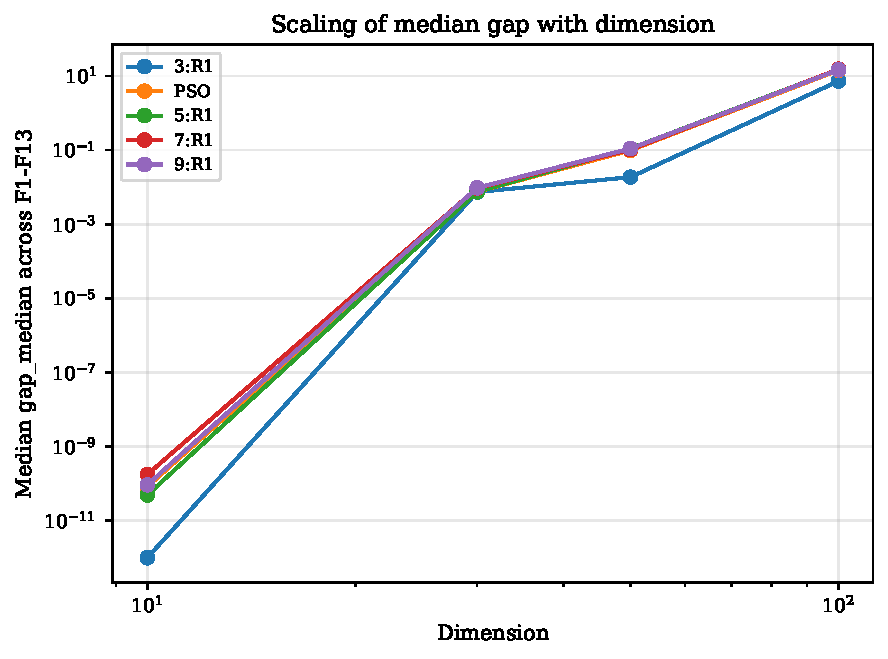
\includegraphics[width=0.85\linewidth]{figures/fig_scaling_curves.pdf}
  \caption{Median normalized gap versus dimension for the five highest mean-rank configurations on S1, including PSO. Both axes are logarithmic.}
  \label{fig:fig_scaling_curves}
\end{figure}

Runtime overhead is estimated as the ratio of independent sample medians for each configuration--instance group, without matching run identifiers. Across the 1,984 FCS--PSO group ratios, median overhead is 27.75\% (interquartile range: 19.81--50.94\%); the 32 configuration-level median ratios range from 25.79\% to 30.90\%. Function-level values in Table~\ref{tab:function_level} refer to the selected best-ranked FCS for that function; the large relative values on some inexpensive fixed-dimensional functions should not be interpreted as hardware-independent computational complexity. All execution times were measured in the same six-worker experiment environment.

\subsection{Dynamic behavior of the controller}
\label{subsec:results_dynamics}

The preceding subsections characterize what each configuration achieves; this one examines its behavior during optimization. Each run records the inertia weight and exploration percentage at every iteration. Exploration percentage (XPL) is defined as $100D_t/D_t^{\max}$, rounded to two decimal places, and corresponds to the normalized diversity ratio $d_t$ used as a controller input. XPL serves as an indicator of swarm dispersion rather than a direct measure of the relative contributions of exploration and exploitation to optimization performance. Figure~\ref{fig:fig_w_trajectories} presents the mean inertia weight and XPL across instances and runs, with XPL aligned to the pre-update swarm state used to compute each $w_t$.

The R1 mean trajectories decline over the run, but they are not the classical linear schedule. The baseline has mean inertia 0.500000 over iterations 0--1000; the existing run summaries give 0.499481, 0.499555, 0.499566, and 0.499835 for FCS-$n$-R1 at $n=3,5,7,9$, respectively. Despite these close overall means, the maximum absolute difference between each R1 mean trajectory and the observed PSO mean trajectory is 0.13480, 0.04194, 0.03315, and 0.02731, respectively. A direct 21-by-21 $(d,p)$ grid evaluation with the implemented controller ($n_{\mathrm{grid}}=501$) found maximum fixed-progress variation across diversity of 0.05325, 0.01160, 0.00973, and 0.00416 for those granularities. A convergence check on an 11-by-11 grid found that increasing the defuzzification grid from 501 to 1001 changed $w$ by less than $10^{-5}$; the observed diversity effects are therefore not numerical integration noise. R1 has diversity-invariant consequents but a weakly diversity-dependent, nonlinear effective schedule. Its leading rank does not establish a benefit of diversity feedback or equivalence to linear PSO. R2, its mirror, inverts the trajectory, while R5 and R6 produce other decreasing schedules and R7 and R8 increase inertia.

The aggregate profiles show a descriptive association between the early-to-late drop in $w$ and mean Friedman rank across the eight patterns (Spearman $\rho=-0.786$, $p=0.021$): patterns with larger declines tend to have better ranks. The end-of-run exploration percentage alone is not associated with rank ($\rho=0.21$, $p=0.61$). R4 and R8, the two patterns that retain the most exploration in the final hundred iterations (5.2\% and 3.6\%, respectively, versus roughly 0.6\% for R1, R3, R5, and R7), also do not converge. These summaries do not identify a causal mechanism; in particular, a nominally neutral consequent axis does not guarantee input independence under min--max inference.

Figure~\ref{fig:fig_convergence_representative} traces this into the convergence profile on four representative instances. On the unimodal F1 at $d=30$, \texttt{FCS-3-R1} remains below the baseline throughout and ends three orders of magnitude lower ($1.7 \times 10^{-9}$ against $7.7 \times 10^{-6}$), while \texttt{FCS-9-R2} stalls at $1.1 \times 10^{3}$ within the first two hundred iterations and never recovers: its weight is still rising when the budget ends. The same contrast appears on F14, where \texttt{FCS-3-R1} settles at a median of 1.99 against 3.97 for the baseline.

\startlandscape
\begin{figure}[H]
  \centering
  \includegraphics[width=\linewidth,height=0.82\textheight,keepaspectratio]{figures/fig_w_trajectories.pdf}
  \caption{Mean inertia weight $w_t$ (top) and normalized diversity XPL (bottom) by pattern and granularity, averaged over 62 instances and 31 runs. XPL is aligned to the pre-update state used for $w_t$. Colour and line style denote progress-consequent direction; PSO is shown as a linear-schedule reference.}
  \label{fig:fig_w_trajectories}
\end{figure}
\finishlandscape

\begin{figure}[!htbp]
  \centering
  \includegraphics[width=\textwidth]{figures/fig_convergence_representative.pdf}
  \caption{Median best fitness by iteration with interquartile bands over 31 runs for four representative instances. Panels compare PSO, \texttt{FCS-3-R1}, the function's best FCS when different, and \texttt{FCS-9-R2}; the vertical axis is symmetric-logarithmic.}
  \label{fig:fig_convergence_representative}
\end{figure}

These trajectories connect the leading ranks to the decreasing-progress consequent family, but do not show that R1 reproduces linear PSO or that its policy is driven solely by iteration progress. Its mean trajectory is nonlinear, and the effective R1 surface varies with diversity through the antecedent firing strengths. The results therefore concern the implemented Mamdani controllers, not an isolated comparison of time-only scheduling against diversity-state feedback.

The mechanism, however, does not imply universal dominance, for two reasons that the same figure makes explicit. On the scalable multimodal F9 at $d=30$, the configuration that wins most instances of that function, \texttt{FCS-5-R2}, descends faster than every alternative during the first two hundred iterations and reaches a median of 38.5, but it then stops improving entirely and finishes behind the baseline, which continues from 87.9 at iteration 200 down to 35.8. An aggressive early transition pays on functions where the budget is the binding constraint and costs on functions where it is not. On F23 the ordering reverses altogether: the baseline and \texttt{FCS-5-R6} both reach the optimum at $-10.54$, while \texttt{FCS-3-R1} stalls at $-3.84$, the same value as the last configuration of the study. A trajectory that is optimal on average is therefore not optimal everywhere, which is the dynamic counterpart of the per-instance heterogeneity of Section~\ref{subsec:results_function}: the 15 configurations that win at least one instance correspond to different ways of scheduling the transition, and none of them fits every landscape.

% Only four representative convergence cases are included in the article. Full trajectories
% remain in the iteration dataset; no separate Supplementary Information file is designated.

%%%%%%%%%%%%%%%%%%%%%%%%%%%%%%%%%%%%%%%%%%
\section{Discussion}
\label{sec:discussion}

\subsection{Rule-Base Structure and Linguistic Granularity}
\label{subsec:discussion_rules_vs_granularity}

Within the evaluated configurations, rule-base structure is closely associated with how inertia control regulates the exploration--exploitation balance in PSO. Patterns with decreasing-progress consequent maps occupy the leading ranks, whereas no progress-neutral or progress-increasing pattern enters the critical-difference group. A decreasing inertia response over the course of the search can reduce the influence of previous particle velocities, potentially favoring a transition from broader exploration toward local refinement. The Holm-adjusted independent-sample comparisons support the observed advantage of decreasing-progress patterns in the matched rule-base contrasts. However, these results concern the implemented control structures and do not establish that progress direction alone determines optimization performance. In particular, the effective inertia response also depends on the interaction of both antecedents under min--max Mamdani inference.


Increasing granularity from $n=3$ to $n=9$ raises the size of a complete two-input rule table from 9 to 81 rules. The finer partition offers more representational distinctions, but those distinctions do not guarantee a better optimization response: the observed rankings and dispersion do not improve consistently with $n$. This separates representational capacity from demonstrated optimization utility. It is consistent with the broader concern for complexity and granularity in interpretable fuzzy modeling \cite{Gacto2011,Castiello2019}, although this experiment measures optimization outcomes, not interpretability scores.

FCS-3-R1 has the best overall mean rank among the evaluated configurations, but its interpretation requires care. Its rule table assigns the same consequent across diversity labels at each progress level; under the implemented min--max Mamdani inference, however, diversity still changes rule firing strengths and therefore the effective output. Its near-0.5 mean inertia is not evidence of a trajectory identical to the 0.9-to-0.1 linear PSO schedule, nor does its ranking isolate a benefit of diversity feedback. The result is specific to this implementation and benchmark; it neither establishes that diversity feedback improves PSO nor shows that diversity feedback is unnecessary in general.

Proposition~\ref{prop:mirror} establishes that designated mirror patterns induce control surfaces complementary about the midpoint of the inertia interval under the stated partition and inference conditions. The Holm-adjusted independent-sample comparisons nevertheless show performance differences between mirror patterns. This contrast shows that symmetry of the controller mapping does not imply equivalent search trajectories or performance: the reflected inertia responses interact with the evolving stochastic swarm. For fuzzy-controller design in bio-inspired optimization, the proposition and empirical comparisons address complementary questions: which relations hold between control surfaces, and how the controlled swarm performs. This supports assessing linguistic granularity and rule-base structure through both mathematical properties and benchmark behavior within the evaluated PSO architecture.

\subsection{Landscape dependence of the best configuration}
\label{subsec:discussion_landscape}

The preferred configuration differs between the evaluated benchmark subsets. The scalable classes show strong observed rank concordance, while the fixed-dimensional class has weak observed concordance with them. Between $S_1$ and $S_2$, observed concordance is weak ($\tau=0.095$, $p=0.451$); the applied test provides insufficient evidence of a positive association but does not establish independence. The leading configurations also differ within these subsets: FCS-3-R5 leads on $S_1$, whereas FCS-5-R6 leads on $S_2$. These findings describe the evaluated benchmark and do not establish or rule out transferability to other problems. The subset specialists both use decreasing-progress consequents but differ in their nominal diversity consequent. At the instance level, the best-performing fuzzy configuration outranks PSO on 50 of 62 cases; 32 of these comparisons are nominally significant and 17 remain significant after Bonferroni correction. Across the 62 instance-specific selections, 34 comparisons are nominally significant. F23 favours PSO in effect size ($A_{12}=0.34$), although its nominal independent-sample $p=0.0234$ does not survive the familywise correction. The instance-wise winners are an oracle comparison: the selected configuration changes after the instance is known.


The class-level results reveal that the relationship between rule-base structure and optimization performance depends on the evaluated problem group. Although decreasing-progress consequent patterns generally achieve better rankings, their relative performance varies across benchmark functions and dimensional regimes. The convergence and inertia-weight trajectories provide a plausible explanation: different consequent mappings produce different inertia-control responses, which may influence how particles maintain their movement and refine candidate solutions throughout the search. A policy that reduces inertia relatively early may favor convergence on some functions but may also restrict continued exploration when further search is needed. Conversely, maintaining higher inertia does not necessarily improve performance, as the observed results also include poorly ranked configurations with increasing-progress consequents. The diversity-related rules further modify these responses, making the resulting search behavior dependent on the complete controller structure rather than on a single linguistic axis. These observations support the importance of considering exploration--exploitation behavior when designing fuzzy controllers for bio-inspired optimization, although they do not identify a causal relationship between specific landscape properties and the success of individual rule patterns.


\subsection{Implications for adaptive fuzzy control}
\label{subsec:discussion_implications}

Roy et al. describe a distinct policy-design approach in which fuzzy feedback policies are optimized on a training benchmark \cite{Roy2024}. The present study instead characterizes performance heterogeneity among predefined static configurations. This heterogeneity motivates future work on online selection, but an instance-wise oracle is not an implementable selector: a deployable method would need to use information available during optimization and be evaluated without selecting configurations retrospectively from test results. No adaptive selector is tested here.

The present ranking also does not isolate the value of diversity feedback. R1 is nominally diversity-agnostic in its consequent table, yet its effective output is diversity-sensitive because both antecedents participate in min--max firing and aggregation. Future comparisons should distinguish consequent-table semantics from the measured sensitivity of the resulting control surface before attributing performance to feedback from a particular input.

\subsection{Study Limitations}
\label{subsec:limitations}

The findings should be interpreted within the experimental conditions considered. All configurations use uniform triangular Ruspini partitions with shoulder functions, a common two-input Mamdani inference architecture, eight predefined consequent patterns, and centroid defuzzification. Other membership-function shapes, overlap levels, and partition structures were not examined. Moreover, the controller regulates only the inertia weight, while the acceleration coefficients, velocity bounds, population size, and computational budget remain fixed. The comparison is restricted to classical PSO with a linear inertia schedule and the unshifted, unrotated F1--F23 benchmark suite. Consequently, the observed configuration rankings should not be assumed to extend to other PSO implementations, fuzzy-controller architectures, or benchmark families.

The analysis also has limitations arising from the benchmark structure and the aggregation of experimental outcomes. Functions evaluated at multiple dimensions are not independent problem families, and the fixed-dimensional subset differs from the scalable subset in more than dimensionality alone. Accordingly, differences between these groups cannot be attributed to individual landscape characteristics. The granularity-by-rule analysis describes the observed dispersion among consequent patterns rather than estimating a general interaction effect. These considerations delimit the interpretation and generalizability of the findings without affecting the descriptive comparisons within the evaluated configurations.

%%%%%%%%%%%%%%%%%%%%%%%%%%%%%%%%%%%%%%%%%%
\section{Conclusions and Future Work}
\label{sec:conclusion}

This study examined how linguistic granularity and rule-base structure relate to the mathematical properties and optimization behavior of static Mamdani fuzzy controllers integrated into particle swarm optimization. By combining a formal characterization of complementary rule-base structures with a controlled experimental evaluation across the Classical F1--F23 benchmark suite, the work provides mathematical and empirical evidence to inform the design of fuzzy inertia-control mechanisms for bio-inspired optimization.

The global ranking places FCS-3-R1 first (mean Friedman rank 4.77) and classical PSO second (6.36); both fall within the same critical-difference group. At the instance level, the best FCS configuration ranks ahead of PSO on 50 of 62 cases, but this is an oracle comparison because the selected configuration changes after the instance is known. The fixed-subset leaders differ: FCS-3-R5 on scalable $S_1$ and FCS-5-R6 on fixed-dimensional $S_2$. Observed rank concordance is weak ($\tau=0.095$, $p=0.451$); the applied test does not establish a positive association, and its non-significant result does not establish independence. These results describe heterogeneity within this benchmark but do not establish or rule out transferability to other problem sets.

FCS-3-R1 is nominally diversity-agnostic in its consequent table, but the implemented min--max Mamdani inference leaves its effective output weakly diversity-dependent. Its leading rank and near-0.5 mean inertia therefore do not demonstrate that diversity feedback improves PSO, nor do they imply a trajectory identical to the classical linear schedule. Within the evaluated configurations, adding explicit diversity trends does not invariably improve ranking; this is not evidence that diversity feedback is unnecessary in general. Proposition~\ref{prop:mirror} characterizes complementary mirror-pair surfaces; the Holm-adjusted independent-sample comparisons show that this structural symmetry does not ensure equivalent optimization performance.

For the evaluated fuzzy controllers and benchmark functions, increasing linguistic granularity did not consistently improve optimization performance or reduce performance differences among rule-base patterns. These findings indicate that greater linguistic resolution, despite increasing the number of rules, does not by itself ensure a more effective inertia-control policy. The organization of the consequent rules is therefore an important consideration when designing fuzzy controllers for bio-inspired optimization. Together with the observed differences across benchmark groups, the results suggest that controller design should consider both the intended inertia response and the characteristics of the optimization problem. These conclusions remain descriptive and specific to the evaluated configurations; they do not establish independent causal effects, statistical equivalence, or a formal granularity-by-rule interaction.


The observed differences among fixed controller configurations provide a basis for investigating dynamic configuration-selection mechanisms in future fuzzy-controlled bio-inspired optimization systems. Such mechanisms could use information available during the search to select among predefined rule-base structures or linguistic granularities according to the evolving optimization state. Unlike the controllers evaluated in this study, whose rule bases and linguistic partitions remain fixed throughout each run, these future approaches would introduce structural changes during optimization and would require independent experimental validation. Further research should also examine the granularity-by-rule interaction through a predefined inferential design, specifying the estimand, experimental unit, and appropriate treatment of repeated measurements. Validation on independent benchmark suites and applied optimization problems would be necessary to assess whether the observed structural relationships extend beyond the classical F1--F23 functions.



\appendixtitles{yes}
\appendixstart
\appendix

\section{Complete Experimental Results and Ranking Diagnostics}
\label{app:instance_results}
The table lists the best-ranked FCS and its comparison with PSO for each of the 62 function--dimension instances. It complements the function-level summary and aggregate RQ4 results in Section~\ref{sec:results}.

\begin{table}[H]
\centering
\footnotesize
\caption{Per-instance FCS--PSO results (part 1 of 3). Ranks use median normalized gap across 33 configurations.}
\label{tab:function_level_full_1}
\setlength{\tabcolsep}{3pt}
\begin{tabular}{llcccccccc}
\toprule
\textbf{Instance} & \textbf{Best FCS} & \boldmath$n$ & \textbf{R} & \textbf{PSO rk.} & \textbf{FCS rk.} & \textbf{PSO gap} & \textbf{FCS gap} & \boldmath$p_{\mathrm{Bonf}}$ & \boldmath$A_{12}$ \\
\midrule
F1\_D10 & \texttt{FCS-3-R1} & 3 & R1 & 5 & 1 & $6.3\!\times10^{-37}$ & $1.4\!\times10^{-44}$ & $<10^{-3}$ & 0.96 \\
F1\_D30 & \texttt{FCS-3-R1} & 3 & R1 & 3 & 1 & $7.7\!\times10^{-6}$ & $1.7\!\times10^{-9}$ & $<10^{-3}$ & 0.97 \\
F1\_D50 & \texttt{FCS-3-R1} & 3 & R1 & 3 & 1 & 0.059 & $1.1\!\times10^{-3}$ & $<10^{-3}$ & 0.99 \\
F1\_D100 & \texttt{FCS-3-R1} & 3 & R1 & 2 & 1 & 16.744 & 10.263 & 1.000 & 0.72 \\
F2\_D10 & \texttt{FCS-3-R1} & 3 & R1 & 6 & 1 & $3.5\!\times10^{-18}$ & $7.7\!\times10^{-25}$ & $<10^{-3}$ & 0.98 \\
F2\_D30 & \texttt{FCS-3-R1} & 3 & R1 & 2 & 1 & $4.5\!\times10^{-4}$ & $5.2\!\times10^{-6}$ & $<10^{-3}$ & 0.98 \\
F2\_D50 & \texttt{FCS-3-R1} & 3 & R1 & 2 & 1 & 0.099 & $8\!\times10^{-3}$ & $<10^{-3}$ & 0.98 \\
F2\_D100 & \texttt{FCS-3-R1} & 3 & R1 & 2 & 1 & 2.357 & 1.375 & $<10^{-3}$ & 0.94 \\
F3\_D10 & \texttt{FCS-5-R5} & 5 & R5 & 9 & 1 & $8.3\!\times10^{-11}$ & $2.8\!\times10^{-15}$ & $<10^{-3}$ & 0.93 \\
F3\_D30 & \texttt{FCS-7-R5} & 7 & R5 & 3 & 1 & 41.57 & 37.246 & 1.000 & 0.58 \\
F3\_D50 & \texttt{FCS-5-R7} & 5 & R7 & 13 & 1 & 1692.014 & 1247.305 & 1.000 & 0.65 \\
F3\_D100 & \texttt{FCS-9-R7} & 9 & R7 & 18 & 1 & $2\!\times10^{4}$ & $1.4\!\times10^{4}$ & 0.027 & 0.82 \\
F4\_D10 & \texttt{FCS-9-R5} & 9 & R5 & 5 & 1 & $1.4\!\times10^{-8}$ & $3.2\!\times10^{-11}$ & $<10^{-3}$ & 0.90 \\
F4\_D30 & \texttt{FCS-9-R1} & 9 & R1 & 6 & 1 & 1.379 & 1.281 & 1.000 & 0.56 \\
F4\_D50 & \texttt{FCS-5-R1} & 5 & R1 & 3 & 1 & 4.347 & 4.234 & 1.000 & 0.56 \\
F4\_D100 & \texttt{FCS-5-R5} & 5 & R5 & 1 & 2 & 14.314 & 14.356 & 1.000 & 0.50 \\
F5\_D10 & \texttt{FCS-3-R1} & 3 & R1 & 5 & 1 & 4.768 & 4.197 & 0.215 & 0.79 \\
F5\_D30 & \texttt{FCS-3-R1} & 3 & R1 & 4 & 1 & 29.198 & 27.947 & 1.000 & 0.50 \\
F5\_D50 & \texttt{FCS-3-R1} & 3 & R1 & 2 & 1 & 150.43 & 116.51 & 1.000 & 0.61 \\
F5\_D100 & \texttt{FCS-3-R1} & 3 & R1 & 2 & 1 & 955.011 & 814.72 & 1.000 & 0.67 \\
F6\_D10 & \texttt{FCS-3-R1} & 3 & R1 & 4 & 1 & $2.8\!\times10^{-32}$ & 0 & 0.006 & 0.82 \\
\bottomrule
\end{tabular}
\par\smallskip
{\raggedright\footnotesize
$p_{\mathrm{Bonf}}$ is the Bonferroni-adjusted two-sided independent-sample Mann--Whitney $U$ $p$-value across 1,984 RQ4 tests. $A_{12}>0.5$ favours the listed FCS because lower fitness is better. Parentheses report configurations sharing the best median-gap rank.\par}
\end{table}
\begin{table}[H]
\centering
\footnotesize
\caption{Per-instance FCS--PSO results (part 2 of 3). Ranks use median normalized gap across 33 configurations.}
\label{tab:function_level_full_2}
\setlength{\tabcolsep}{3pt}
\begin{tabular}{llcccccccc}
\toprule
\textbf{Instance} & \textbf{Best FCS} & \boldmath$n$ & \textbf{R} & \textbf{PSO rk.} & \textbf{FCS rk.} & \textbf{PSO gap} & \textbf{FCS gap} & \boldmath$p_{\mathrm{Bonf}}$ & \boldmath$A_{12}$ \\
\midrule
F6\_D30 & \texttt{FCS-3-R1} & 3 & R1 & 2 & 1 & $2.4\!\times10^{-6}$ & $1.9\!\times10^{-9}$ & $<10^{-3}$ & 0.99 \\
F6\_D50 & \texttt{FCS-3-R1} & 3 & R1 & 2 & 1 & 0.046 & $1.1\!\times10^{-3}$ & $<10^{-3}$ & 0.97 \\
F6\_D100 & \texttt{FCS-3-R1} & 3 & R1 & 2 & 1 & 22.053 & 7.284 & $<10^{-3}$ & 0.93 \\
F7\_D10 & \texttt{FCS-7-R6} & 7 & R6 & 8 & 1 & $1.3\!\times10^{-3}$ & $1\!\times10^{-3}$ & 1.000 & 0.56 \\
F7\_D30 & \texttt{FCS-5-R1} & 5 & R1 & 1 & 2 & $9\!\times10^{-3}$ & $9.1\!\times10^{-3}$ & 1.000 & 0.52 \\
F7\_D50 & \texttt{FCS-3-R1} & 3 & R1 & 2 & 1 & 0.028 & 0.027 & 1.000 & 0.53 \\
F7\_D100 & \texttt{FCS-5-R1} & 5 & R1 & 4 & 1 & 0.142 & 0.132 & 1.000 & 0.55 \\
F8\_D10 & \texttt{FCS-9-R8} & 9 & R8 & 6 & 1 & 0.415 & 0.396 & 1.000 & 0.56 \\
F8\_D30 & \texttt{FCS-7-R3} & 7 & R3 & 12 & 1 & 0.495 & 0.465 & 1.000 & 0.55 \\
F8\_D50 & \texttt{FCS-3-R1} & 3 & R1 & 1 & 2 & 0.483 & 0.491 & 1.000 & 0.43 \\
F8\_D100 & \texttt{FCS-5-R6} & 5 & R6 & 1 & 2 & 0.502 & 0.503 & 1.000 & 0.54 \\
F9\_D10 & \texttt{FCS-5-R2} & 5 & R2 & 11 & 1 & 10.945 & 8.955 & 1.000 & 0.59 \\
F9\_D30 & \texttt{FCS-5-R5} & 5 & R5 & 7 & 1 & 35.818 & 31.853 & 1.000 & 0.56 \\
F9\_D50 & \texttt{FCS-3-R5} & 3 & R5 & 14 & 1 & 67.66 & 55.771 & 1.000 & 0.68 \\
F9\_D100 & \texttt{FCS-7-R5} & 7 & R5 & 4 & 1 & 132.303 & 122.623 & 1.000 & 0.61 \\
F10\_D10 & \texttt{FCS-3-R1} (6 tied) & 3 & R1 & 4 & 4 & $4\!\times10^{-15}$ & $4\!\times10^{-15}$ & 1.000 & 0.45 \\
F10\_D30 & \texttt{FCS-3-R1} & 3 & R1 & 2 & 1 & $6.6\!\times10^{-4}$ & $1.5\!\times10^{-5}$ & $<10^{-3}$ & 0.93 \\
F10\_D50 & \texttt{FCS-3-R1} & 3 & R1 & 4 & 1 & 0.522 & 0.019 & 0.094 & 0.80 \\
F10\_D100 & \texttt{FCS-3-R1} & 3 & R1 & 3 & 1 & 2.192 & 1.966 & 1.000 & 0.74 \\
F11\_D10 & \texttt{FCS-9-R1} & 9 & R1 & 10 & 1 & 0.091 & 0.069 & 1.000 & 0.64 \\
F11\_D30 & \texttt{FCS-7-R1} & 7 & R1 & 5 & 1 & $7.5\!\times10^{-3}$ & $1.4\!\times10^{-3}$ & 1.000 & 0.54 \\
\bottomrule
\end{tabular}
\par\smallskip
{\raggedright\footnotesize
$p_{\mathrm{Bonf}}$ is the Bonferroni-adjusted two-sided independent-sample Mann--Whitney $U$ $p$-value across 1,984 RQ4 tests. $A_{12}>0.5$ favours the listed FCS because lower fitness is better. Parentheses report configurations sharing the best median-gap rank.\par}
\end{table}
\begin{table}[H]
\centering
\footnotesize
\caption{Per-instance FCS--PSO results (part 3 of 3). Ranks use median normalized gap across 33 configurations.}
\label{tab:function_level_full_3}
\setlength{\tabcolsep}{3pt}
\begin{tabular}{llcccccccc}
\toprule
\textbf{Instance} & \textbf{Best FCS} & \boldmath$n$ & \textbf{R} & \textbf{PSO rk.} & \textbf{FCS rk.} & \textbf{PSO gap} & \textbf{FCS gap} & \boldmath$p_{\mathrm{Bonf}}$ & \boldmath$A_{12}$ \\
\midrule
F11\_D50 & \texttt{FCS-3-R1} & 3 & R1 & 3 & 1 & 0.064 & 0.012 & $<10^{-3}$ & 0.91 \\
F11\_D100 & \texttt{FCS-3-R1} & 3 & R1 & 2 & 1 & 1.168 & 1.042 & 0.004 & 0.85 \\
F12\_D10 & \texttt{FCS-3-R1} & 3 & R1 & 2 & 1 & $4.8\!\times10^{-32}$ & $4.7\!\times10^{-32}$ & 0.284 & 0.77 \\
F12\_D30 & \texttt{FCS-3-R1} & 3 & R1 & 2 & 1 & $1.2\!\times10^{-8}$ & $2.1\!\times10^{-11}$ & 0.065 & 0.81 \\
F12\_D50 & \texttt{FCS-7-R1} & 7 & R1 & 1 & 2 & $4.1\!\times10^{-4}$ & $4.9\!\times10^{-4}$ & 1.000 & 0.49 \\
F12\_D100 & \texttt{FCS-5-R1} & 5 & R1 & 3 & 1 & 2.769 & 2.313 & 1.000 & 0.67 \\
F13\_D10 & \texttt{FCS-3-R1} & 3 & R1 & 3 & 1 & $1.8\!\times10^{-32}$ & $1.3\!\times10^{-32}$ & 0.126 & 0.76 \\
F13\_D30 & \texttt{FCS-3-R1} & 3 & R1 & 2 & 1 & $2.4\!\times10^{-6}$ & $9.4\!\times10^{-9}$ & 1.000 & 0.65 \\
F13\_D50 & \texttt{FCS-3-R1} & 3 & R1 & 3 & 1 & 0.025 & $8.9\!\times10^{-3}$ & 0.112 & 0.80 \\
F13\_D100 & \texttt{FCS-3-R1} & 3 & R1 & 3 & 1 & 16.942 & 9.312 & 1.000 & 0.73 \\
F14\_D2 & \texttt{FCS-3-R1} (6 tied) & 3 & R1 & 27 & 3 & 2.968 & 0.992 & 1.000 & 0.58 \\
F15\_D4 & \texttt{FCS-3-R1} & 3 & R1 & 11 & 1 & $7.5\!\times10^{-6}$ & $7.5\!\times10^{-6}$ & 1.000 & 0.75 \\
F16\_D2 & \texttt{FCS-3-R1} (32 tied) & 3 & R1 & 17 & 17 & 0 & 0 & 1.000 & 0.56 \\
F17\_D2 & \texttt{FCS-3-R1} (32 tied) & 3 & R1 & 17 & 17 & 0 & 0 & 1.000 & 0.50 \\
F18\_D2 & \texttt{FCS-3-R1} (28 tied) & 3 & R1 & 15 & 15 & 0 & 0 & 1.000 & 0.45 \\
F19\_D3 & \texttt{FCS-3-R1} (32 tied) & 3 & R1 & 17 & 17 & 0 & 0 & 1.000 & 0.56 \\
F20\_D6 & \texttt{FCS-3-R1} (27 tied) & 3 & R1 & 14 & 14 & 0 & 0 & 1.000 & 0.55 \\
F21\_D4 & \texttt{FCS-7-R1} & 7 & R1 & 24 & 1 & 0.736 & 0 & 1.000 & 0.61 \\
F22\_D4 & \texttt{FCS-3-R6} (2 tied) & 3 & R6 & 20 & 1 & 0.642 & 0 & 1.000 & 0.57 \\
F23\_D4 & \texttt{FCS-5-R6} & 5 & R6 & 1 & 2 & 0 & $1.7\!\times10^{-16}$ & 1.000 & 0.34 \\
\bottomrule
\end{tabular}
\par\smallskip
{\raggedright\footnotesize
$p_{\mathrm{Bonf}}$ is the Bonferroni-adjusted two-sided independent-sample Mann--Whitney $U$ $p$-value across 1,984 RQ4 tests. $A_{12}>0.5$ favours the listed FCS because lower fitness is better. Parentheses report configurations sharing the best median-gap rank.\par}
\end{table}


\begin{figure}[!htbp]
	\begin{adjustwidth}{-\extralength}{0cm}
	\centering
	\includegraphics[width=\fulllength,height=0.90\textheight,keepaspectratio]{figures/fig_function_heatmap.png}
	\end{adjustwidth}
	\caption{Per-instance Friedman ranks of 33 configurations across 62 instances, computed on median normalized gap (rank 1 = best). Columns are ordered by mean rank; vertical rules bracket PSO and the horizontal rule separates S1 and S2. Green denotes better ranks.}
	\label{fig:fig_function_heatmap}
\end{figure}

\begin{figure}[p]
	\begin{adjustwidth}{-\extralength}{0cm}
	\centering
	\includegraphics[width=0.90\fulllength,height=0.86\textheight,keepaspectratio]{figures/fig_h4_independent_outcomes.pdf}
	\end{adjustwidth}
	\caption{Nominal independent-sample Mann--Whitney outcomes against PSO for the ten configurations ranked by Bonferroni-significant wins. Bars cover 62 instances; green, grey, and red denote wins, non-significant comparisons, and losses at $p<0.05$.}
	\label{fig:fig_h4_independent_outcomes}
\end{figure}

\clearpage

\section{Extended Performance and Dispersion Diagnostics}
\label{app:dispersion_atlas}
Figure~\ref{fig:fig_mean_dispersion} shows four representative instances; the atlas that follows covers all 62 function--dimension instances. Each point is one fixed configuration, lower-left indicates lower mean gap and variability, both axes are logarithmic, and zero gaps use a $10^{-12}$ floor. The scalable functions share axis limits across their four dimensions. The representative cases are interpreted in Section~\ref{subsec:results_robustness}.

\begin{figure}[!htbp]
	\begin{adjustwidth}{-\extralength}{0cm}
	\centering
	\includegraphics[width=0.90\fulllength,height=0.82\textheight,keepaspectratio]{figures/fig_mean_dispersion_representative.pdf}
	\end{adjustwidth}
	\caption{Mean normalized gap versus run-to-run standard deviation over 31 runs for four instances. Both axes are logarithmic; zero gaps use a $10^{-12}$ display floor. Colour denotes pattern, marker shape granularity, the star PSO, and the open circle the function's best FCS.}
	\label{fig:fig_mean_dispersion}
\end{figure}

\begin{figure}[p]
  \begin{adjustwidth}{-\extralength}{0cm}
  \centering
  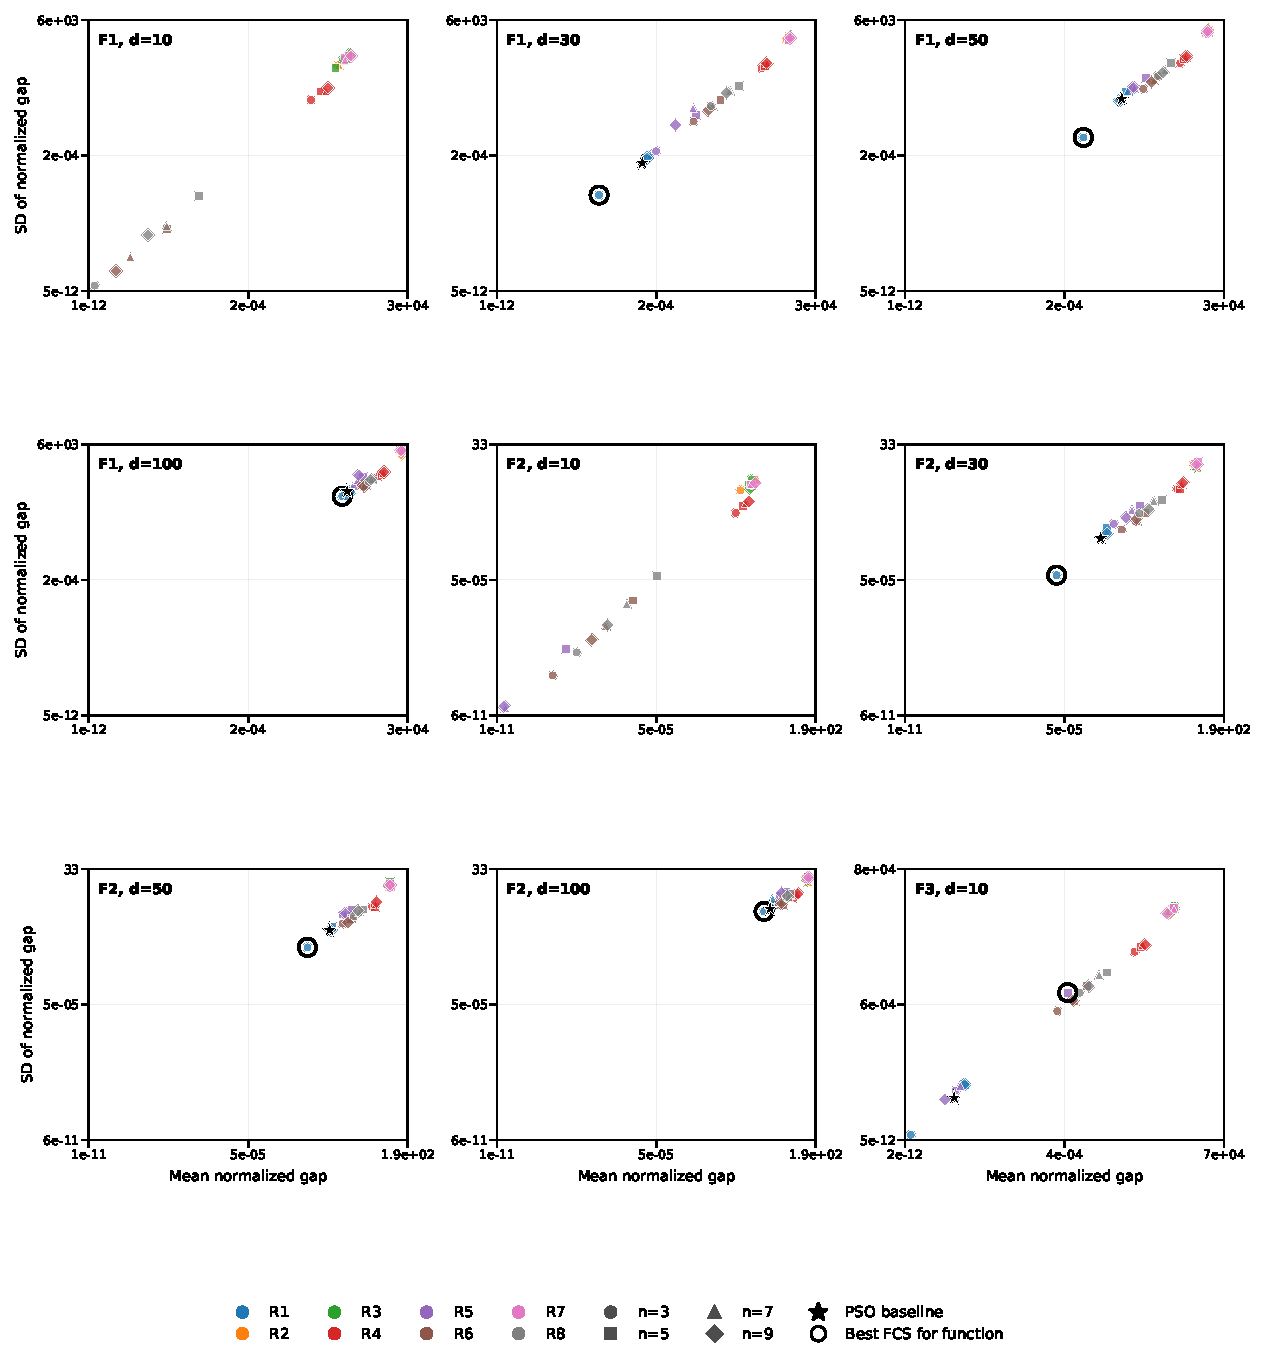
\includegraphics[page=1,width=\fulllength,height=0.82\textheight,keepaspectratio]{figures/appendices/fig_mean_dispersion_by_function.pdf}
  \end{adjustwidth}
  \caption{Mean-versus-dispersion panels for the function--dimension instances identified in each subplot.}
  \label{fig:app_dispersion_1}
\end{figure}
\clearpage

\begin{figure}[p]
  \begin{adjustwidth}{-\extralength}{0cm}
  \centering
  \includegraphics[page=2,width=\fulllength,height=0.82\textheight,keepaspectratio]{figures/appendices/fig_mean_dispersion_by_function.pdf}
  \end{adjustwidth}
  \caption{Mean-versus-dispersion panels for the function--dimension instances identified in each subplot.}
  \label{fig:app_dispersion_2}
\end{figure}
\clearpage

\begin{figure}[p]
  \begin{adjustwidth}{-\extralength}{0cm}
  \centering
  \includegraphics[page=3,width=\fulllength,height=0.82\textheight,keepaspectratio]{figures/appendices/fig_mean_dispersion_by_function.pdf}
  \end{adjustwidth}
  \caption{Mean-versus-dispersion panels for the function--dimension instances identified in each subplot.}
  \label{fig:app_dispersion_3}
\end{figure}
\clearpage

\begin{figure}[p]
  \begin{adjustwidth}{-\extralength}{0cm}
  \centering
  \includegraphics[page=4,width=\fulllength,height=0.82\textheight,keepaspectratio]{figures/appendices/fig_mean_dispersion_by_function.pdf}
  \end{adjustwidth}
  \caption{Mean-versus-dispersion panels for the function--dimension instances identified in each subplot.}
  \label{fig:app_dispersion_4}
\end{figure}
\clearpage

\begin{figure}[p]
  \begin{adjustwidth}{-\extralength}{0cm}
  \centering
  \includegraphics[page=5,width=\fulllength,height=0.82\textheight,keepaspectratio]{figures/appendices/fig_mean_dispersion_by_function.pdf}
  \end{adjustwidth}
  \caption{Mean-versus-dispersion panels for the function--dimension instances identified in each subplot.}
  \label{fig:app_dispersion_5}
\end{figure}
\clearpage

\begin{figure}[p]
  \begin{adjustwidth}{-\extralength}{0cm}
  \centering
  \includegraphics[page=6,width=\fulllength,height=0.82\textheight,keepaspectratio]{figures/appendices/fig_mean_dispersion_by_function.pdf}
  \end{adjustwidth}
  \caption{Mean-versus-dispersion panels for the function--dimension instances identified in each subplot.}
  \label{fig:app_dispersion_6}
\end{figure}
\clearpage

\begin{figure}[p]
  \begin{adjustwidth}{-\extralength}{0cm}
  \centering
  \includegraphics[page=7,width=\fulllength,height=0.82\textheight,keepaspectratio]{figures/appendices/fig_mean_dispersion_by_function.pdf}
  \end{adjustwidth}
  \caption{Mean-versus-dispersion panels for the function--dimension instances identified in each subplot.}
  \label{fig:app_dispersion_7}
\end{figure}
\clearpage


\section{Fuzzy Controller Configurations and Control Surfaces}
\label{app:controller_configs}
This appendix provides the remaining rule-consequent matrices, effective Mamdani control surfaces, and workflow diagram referenced in Section~\ref{sec:framework}. All configurations use the common two-input architecture and inference procedure defined in the main text.

% Remaining controller configuration and workflow figures, integrated in Appendix C.

\begin{figure}[!htbp]
  \begin{adjustwidth}{-\extralength}{0cm}
  \centering
  \includegraphics[width=\fulllength,height=0.88\textheight,keepaspectratio]{figures/04_fuzzy_rules_panel_5labels.png}
  \end{adjustwidth}
  \caption{Rule-base consequents R1--R8 at $n=5$. Rows denote diversity labels and columns denote progress labels.}
  \label{fig:rule_panel_5}
\end{figure}

\begin{figure}[p]
  \begin{adjustwidth}{-\extralength}{0cm}
  \centering
  \includegraphics[width=\fulllength,height=0.88\textheight,keepaspectratio]{figures/04_fuzzy_rules_panel_7labels.png}
  \end{adjustwidth}
  \caption{Rule-base consequents R1--R8 at $n=7$. Rows denote diversity labels and columns denote progress labels.}
  \label{fig:rule_panel_7}
\end{figure}

\begin{figure}[p]
  \begin{adjustwidth}{-\extralength}{0cm}
  \centering
  \includegraphics[width=\fulllength,height=0.88\textheight,keepaspectratio]{figures/04_fuzzy_rules_panel_9labels.png}
  \end{adjustwidth}
  \caption{Rule-base consequents R1--R8 at $n=9$. Rows denote diversity labels and columns denote progress labels.}
  \label{fig:rule_panel_9}
\end{figure}

\begin{figure}[p]
  \centering
  \includegraphics[width=0.92\textwidth,height=0.82\textheight,keepaspectratio]{figures/11_3d_surface_panel_3labels_I1.png}
  \caption{Effective Mamdani inertia-weight surfaces for R1--R8 at $n=3$, over diversity and progress; $w\in[0.1,0.9]$.}
  \label{fig:surface_panel_3}
\end{figure}

\begin{figure}[p]
  \centering
  \includegraphics[width=0.92\textwidth,height=0.82\textheight,keepaspectratio]{figures/11_3d_surface_panel_7labels_I1.png}
  \caption{Effective Mamdani inertia-weight surfaces for R1--R8 at $n=7$, over diversity and progress; $w\in[0.1,0.9]$.}
  \label{fig:surface_panel_7}
\end{figure}

\begin{figure}[p]
  \centering
  \includegraphics[width=0.92\textwidth,height=0.82\textheight,keepaspectratio]{figures/11_3d_surface_panel_9labels_I1.png}
  \caption{Effective Mamdani inertia-weight surfaces for R1--R8 at $n=9$, over diversity and progress; $w\in[0.1,0.9]$.}
  \label{fig:surface_panel_9}
\end{figure}

\usetikzlibrary{positioning,fit,shapes.geometric}
\begin{figure}[p]
  \begin{adjustwidth}{-\extralength}{0cm}
  \centering
  \begin{tikzpicture}[
    process/.style={draw=black,fill=white,rectangle,align=center,text width=12cm,minimum height=9mm,inner sep=5pt,font=\small},
    controller/.style={draw=black,fill=white,rectangle,align=center,text width=9cm,minimum height=8mm,inner sep=4pt,font=\small},
    decision/.style={draw=black,fill=white,diamond,aspect=2.8,align=center,inner sep=2pt,font=\small},
    flow/.style={->,>=stealth,thick,draw=black},
    node distance=5mm]
    \node[process] (initialize) {Initialize the swarm; evaluate particles; set personal and global bests};
    \node[process,below=of initialize] (state) {Compute controller inputs: normalized diversity $d_t$ and progress $p_t$};
    \node[controller,below=13mm of state] (fuzzify) {\textbf{Fuzzification:} map $d_t$ and $p_t$ to membership grades};
    \node[controller,below=of fuzzify] (infer) {\textbf{Rule inference:} evaluate the selected rule base $R_k$};
    \node[controller,below=of infer] (defuzzify) {\textbf{Defuzzification:} centroid method; rescale $w_t$ to $[0.1,0.9]$};
    \node[draw=black,dashed,rectangle,fit=(fuzzify)(infer)(defuzzify),inner sep=7mm,
      label={[anchor=south west,font=\small]north west:\textbf{Fuzzy inertia controller}}] (fis) {};
    \node[process,below=12mm of fis] (particle) {For each particle: apply PSO update; evaluate fitness; update personal best};
    \node[process,below=of particle] (swarm) {After all particles: update global best and advance the iteration};
    \node[decision,below=of swarm] (continue) {$t<T_{\max}$?};
    \node[process,below=of continue] (result) {Return the best position $\mathbf{g}$ and objective value $f(\mathbf{g})$};
    \draw[flow] (initialize) -- (state);
    \draw[flow] (state.south) -- (fis.north);
    \draw[flow] (fuzzify) -- (infer);
    \draw[flow] (infer) -- (defuzzify);
    \draw[flow] (fis.south) -- (particle.north);
    \draw[flow] (particle) -- (swarm);
    \draw[flow] (swarm) -- (continue);
    \draw[flow] (continue) -- node[right,font=\footnotesize]{no} (result);
    \draw[flow] (continue.east) -- node[above,font=\footnotesize]{yes} ++(15mm,0) -- ++(60mm,0) |- (state.east);
  \end{tikzpicture}
  \end{adjustwidth}
  \caption{PSO--FCS workflow: the common two-input fuzzy controller returns one inertia weight shared by all particles.}
  \label{fig:pso_fcs_loop}
\end{figure}

\clearpage

\section{Benchmark Landscape Visualizations}
\label{app:benchmark_landscapes}
The panels below are illustrative objective landscapes and two-coordinate slices; the benchmark functions, dimensions, domains, and solver reference optima are defined in Tables~\ref{tab:benchmark_scalable}--\ref{tab:benchmark_fixed} in Section~\ref{subsec:benchmarks}. They do not constitute quantitative landscape characterization.

% Two-dimensional functions show the full landscape; higher-dimensional functions show a slice.
\begin{figure}[p]
  \begin{adjustwidth}{-\extralength}{0cm}
  \centering
  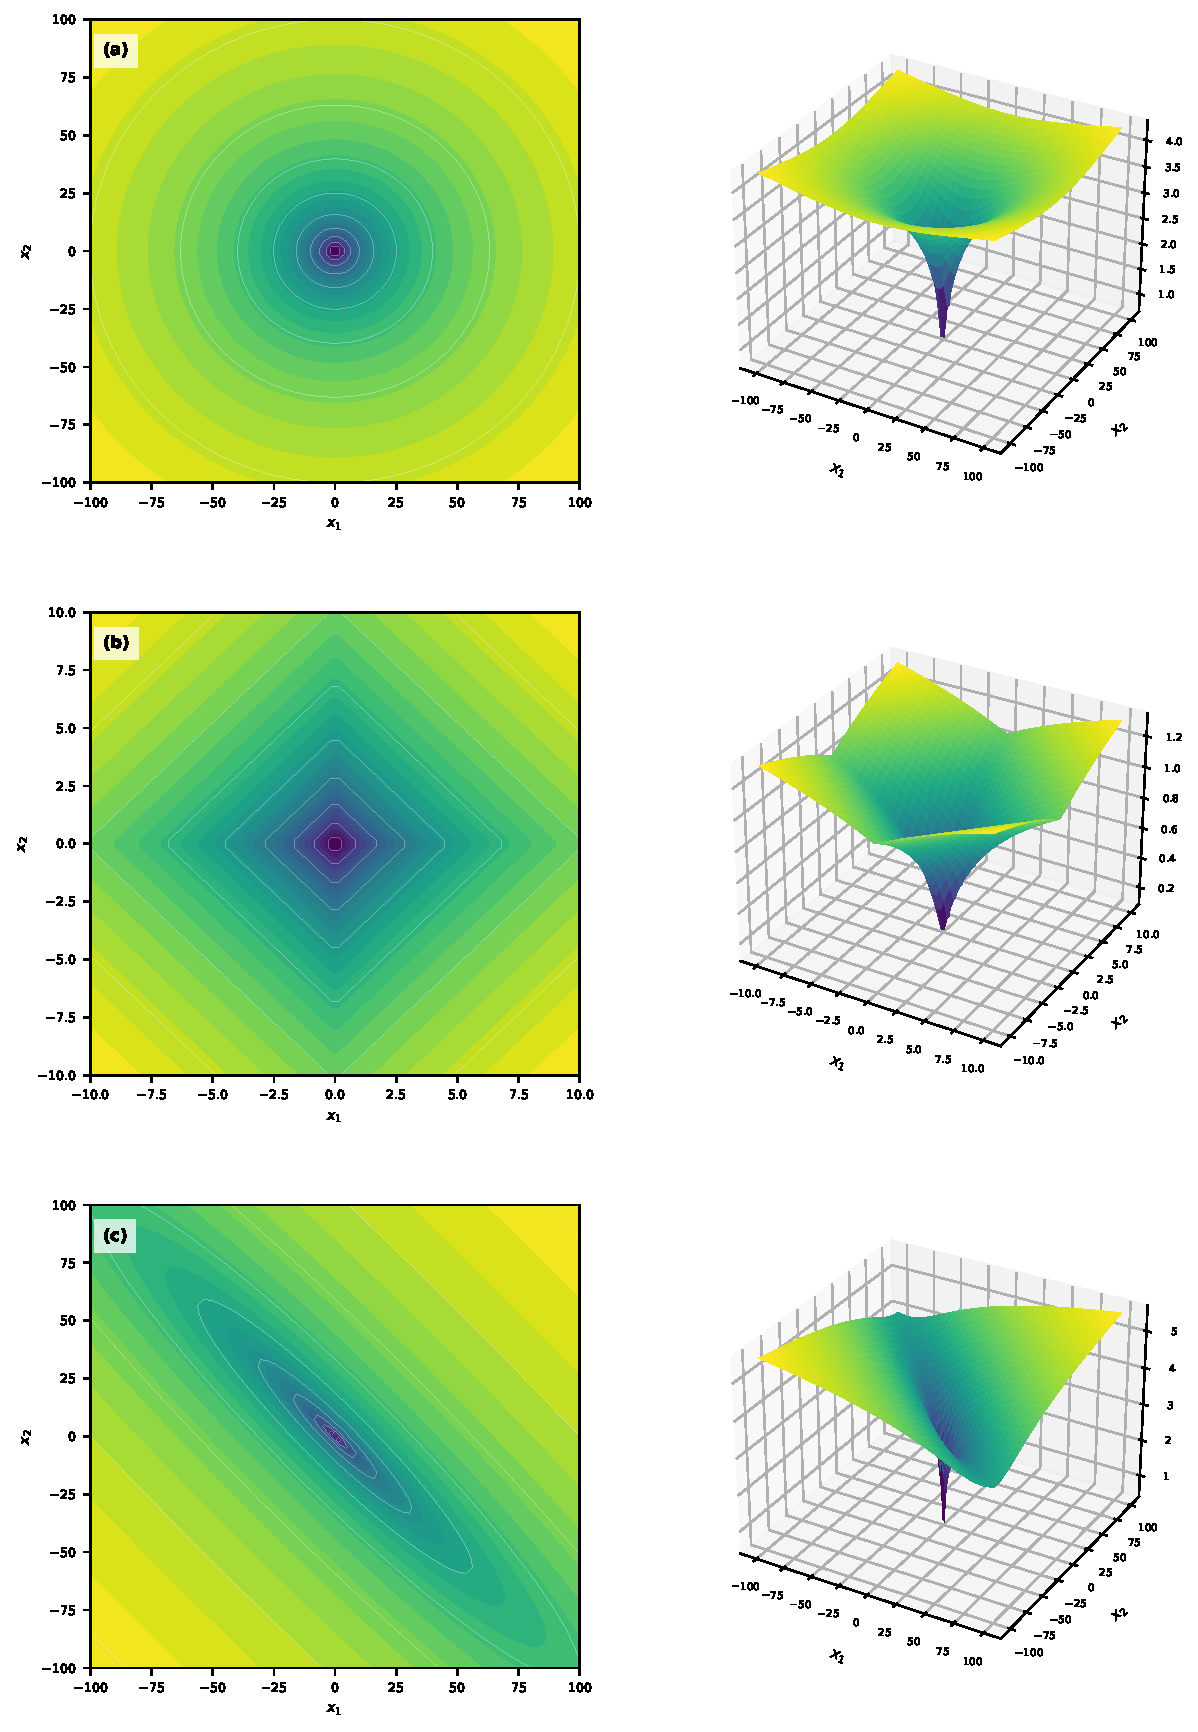
\includegraphics[width=\fulllength,height=0.84\textheight,keepaspectratio]{figures/landscapes_body/landscape_body_group_01.pdf}
  \end{adjustwidth}
  \caption{Benchmark objective landscapes and two-dimensional slices: (a) F1 (Sphere, $d=10$); (b) F2 (Schwefel 2.22, $d=10$); (c) F3 (Schwefel 1.2, $d=10$). Contours are shown at left and 3-D surfaces at right; colour shows log-compressed objective excess on function-specific scales. For $d>2$, other coordinates are fixed at the midpoint of the solver bounds. Bounds and reference optima are listed in Tables~\ref{tab:benchmark_scalable}--\ref{tab:benchmark_fixed}.}
  \label{fig:landscape_body_01}
\end{figure}
\clearpage

\begin{figure}[p]
  \begin{adjustwidth}{-\extralength}{0cm}
  \centering
  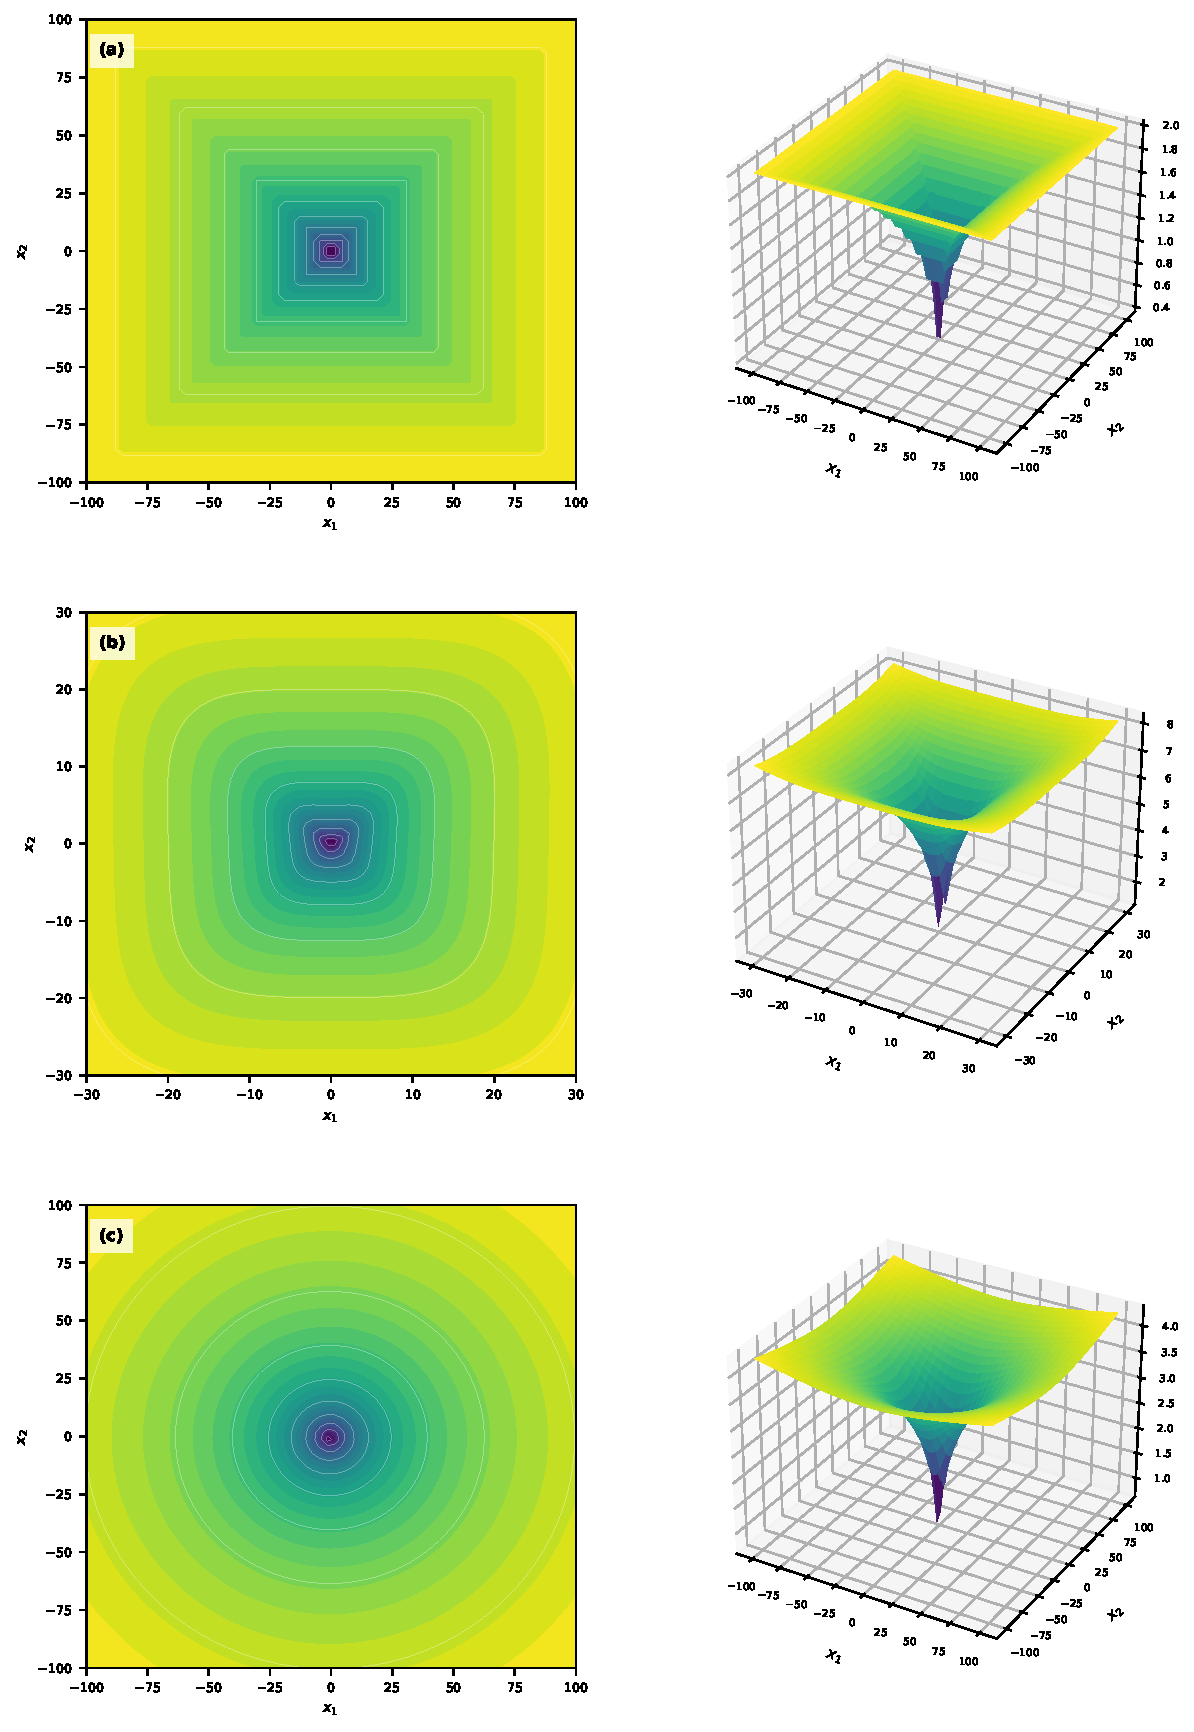
\includegraphics[width=\fulllength,height=0.84\textheight,keepaspectratio]{figures/landscapes_body/landscape_body_group_02.pdf}
  \end{adjustwidth}
  \caption{Benchmark objective landscapes and two-dimensional slices: (a) F4 (Schwefel 2.21, $d=10$); (b) F5 (Rosenbrock, $d=10$); (c) F6 (Shifted step, $d=10$). Contours are shown at left and 3-D surfaces at right; colour shows log-compressed objective excess on function-specific scales. For $d>2$, other coordinates are fixed at the midpoint of the solver bounds. Bounds and reference optima are listed in Tables~\ref{tab:benchmark_scalable}--\ref{tab:benchmark_fixed}.}
  \label{fig:landscape_body_02}
\end{figure}
\clearpage

\begin{figure}[p]
  \begin{adjustwidth}{-\extralength}{0cm}
  \centering
  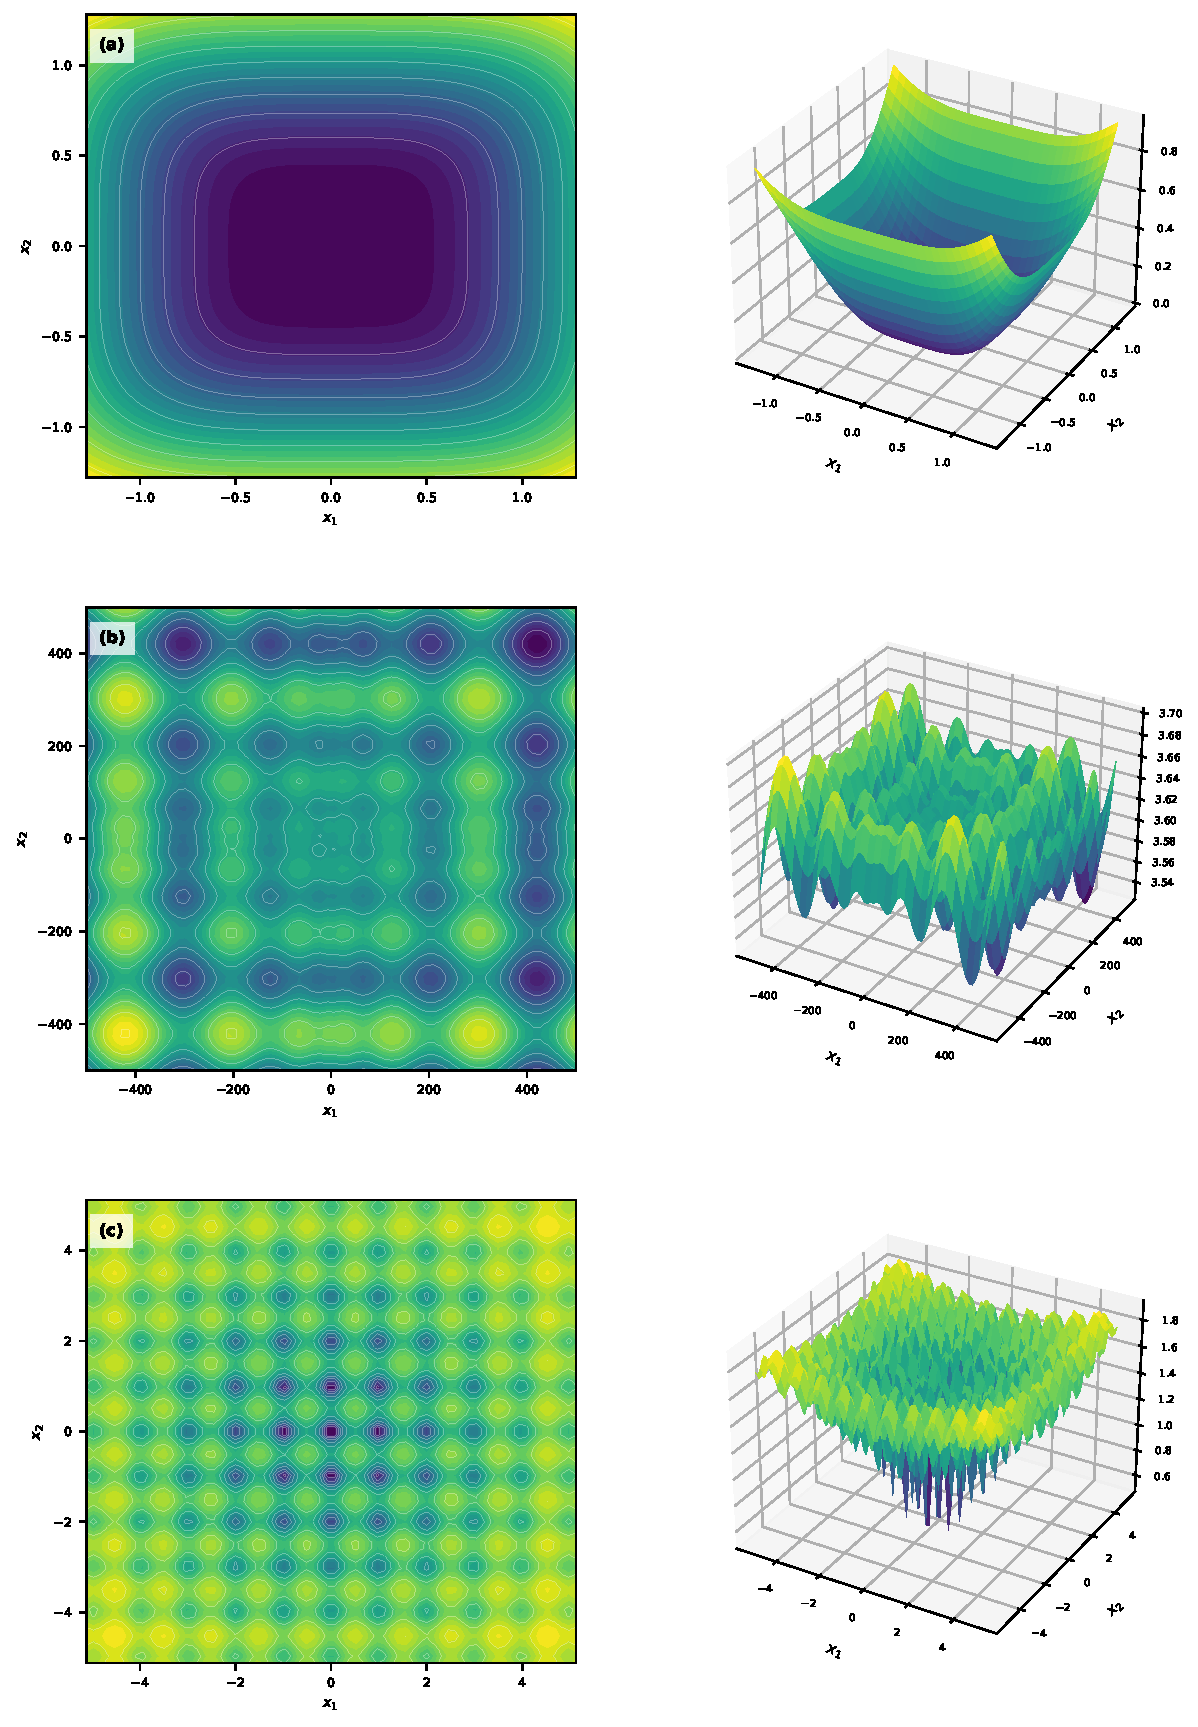
\includegraphics[width=\fulllength,height=0.84\textheight,keepaspectratio]{figures/landscapes_body/landscape_body_group_03.pdf}
  \end{adjustwidth}
  \caption{Benchmark objective landscapes and two-dimensional slices: (a) F7 (Quartic with noise, $d=10$); (b) F8 (Schwefel 2.26, $d=10$); (c) F9 (Rastrigin, $d=10$). Contours are shown at left and 3-D surfaces at right; colour shows log-compressed objective excess on function-specific scales. For $d>2$, other coordinates are fixed at the midpoint of the solver bounds. Bounds and reference optima are listed in Tables~\ref{tab:benchmark_scalable}--\ref{tab:benchmark_fixed}. The F7 panel uses the expected objective, including its 0.5 uniform-noise offset.}
  \label{fig:landscape_body_03}
\end{figure}
\clearpage

\begin{figure}[p]
  \begin{adjustwidth}{-\extralength}{0cm}
  \centering
  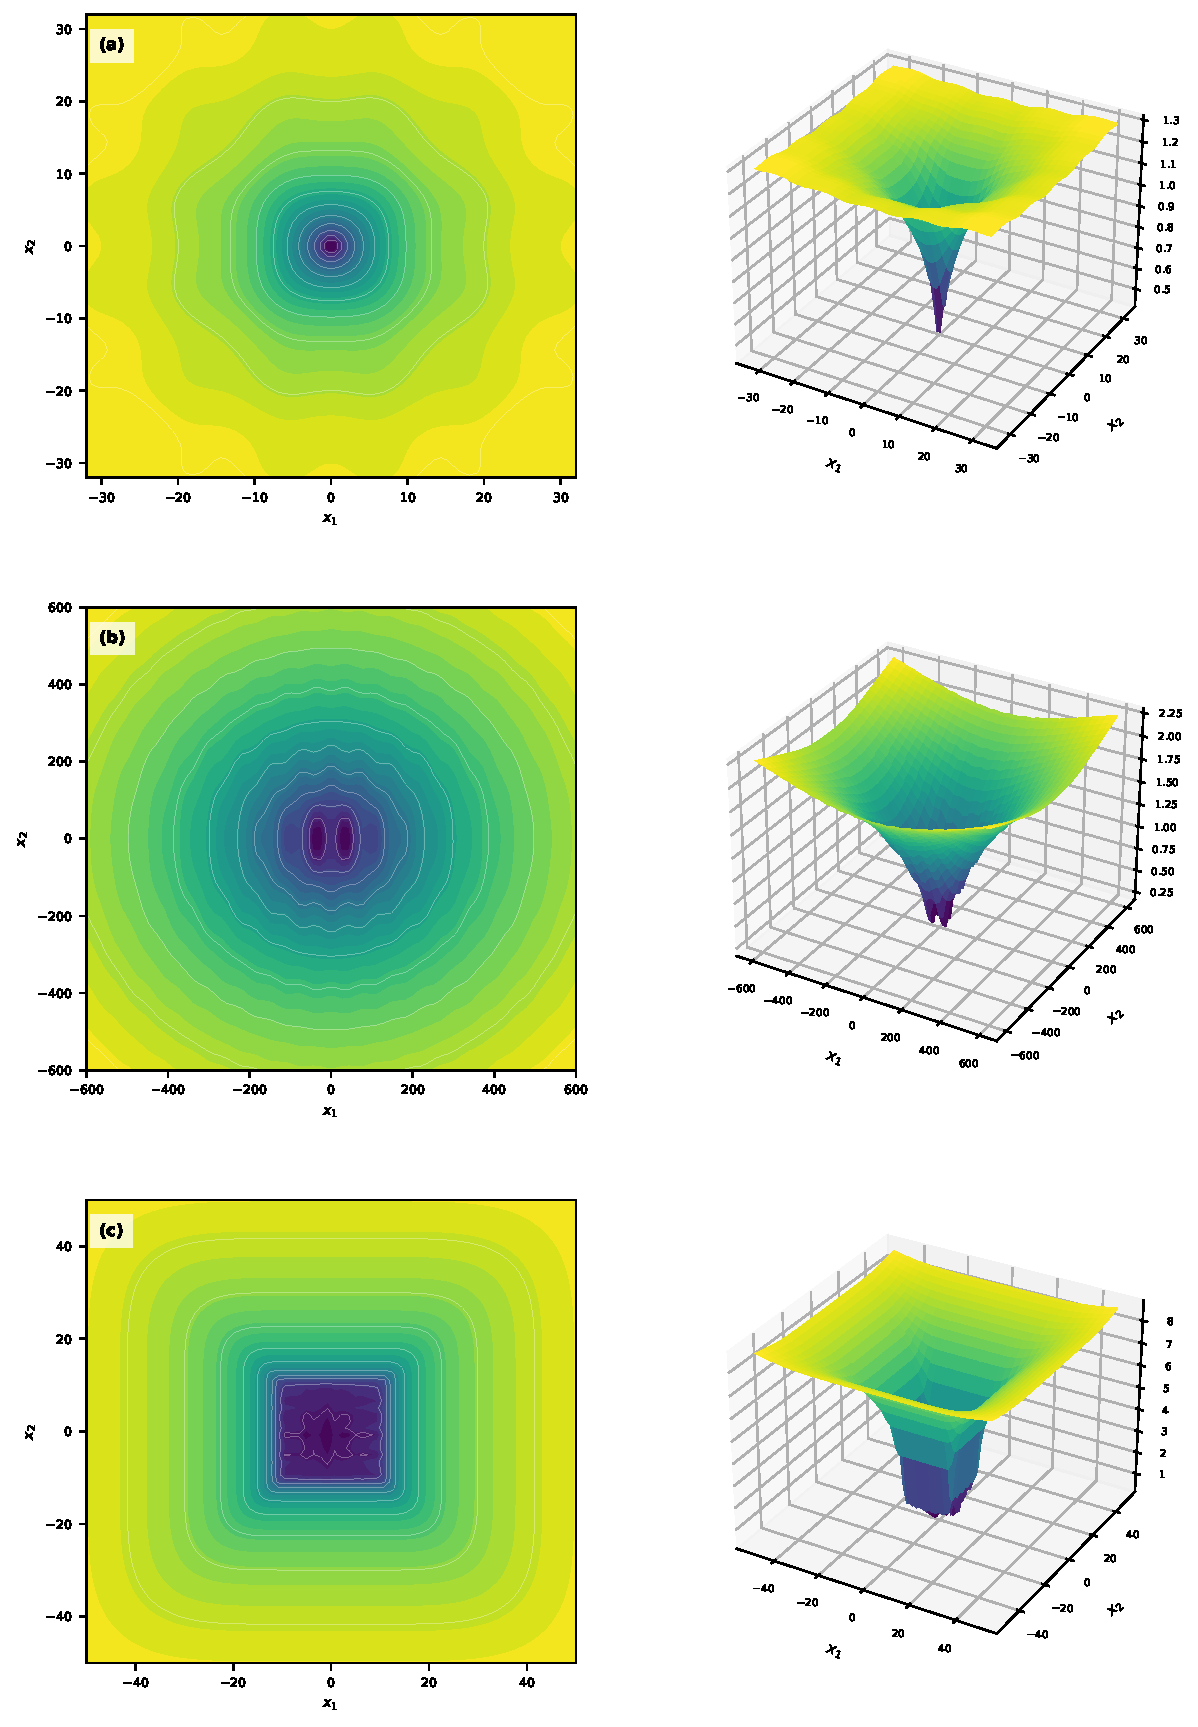
\includegraphics[width=\fulllength,height=0.84\textheight,keepaspectratio]{figures/landscapes_body/landscape_body_group_04.pdf}
  \end{adjustwidth}
  \caption{Benchmark objective landscapes and two-dimensional slices: (a) F10 (Ackley, $d=10$); (b) F11 (Griewank, $d=10$); (c) F12 (Penalized 1, $d=10$). Contours are shown at left and 3-D surfaces at right; colour shows log-compressed objective excess on function-specific scales. For $d>2$, other coordinates are fixed at the midpoint of the solver bounds. Bounds and reference optima are listed in Tables~\ref{tab:benchmark_scalable}--\ref{tab:benchmark_fixed}.}
  \label{fig:landscape_body_04}
\end{figure}
\clearpage

\begin{figure}[p]
  \begin{adjustwidth}{-\extralength}{0cm}
  \centering
  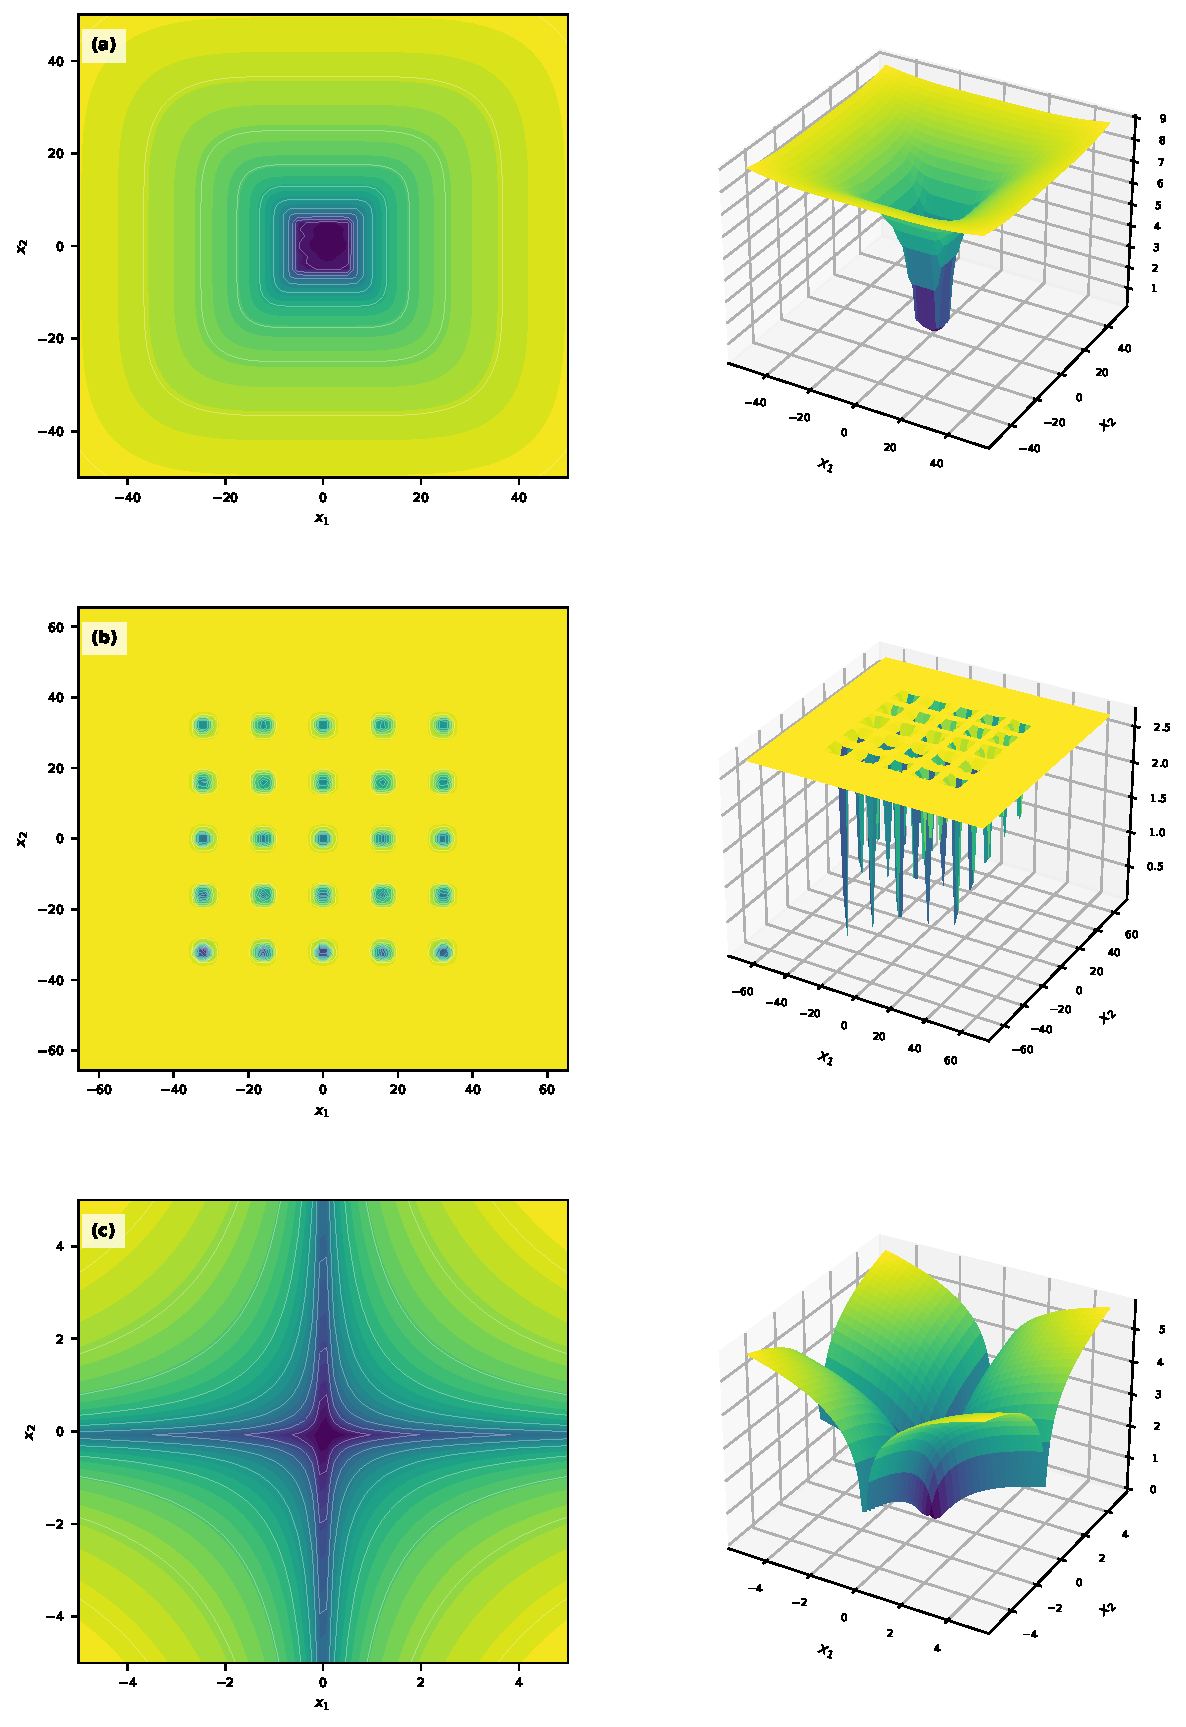
\includegraphics[width=\fulllength,height=0.84\textheight,keepaspectratio]{figures/landscapes_body/landscape_body_group_05.pdf}
  \end{adjustwidth}
  \caption{Benchmark objective landscapes and two-dimensional slices: (a) F13 (Penalized 2, $d=10$); (b) F14 (Shekel foxholes, $d=2$); (c) F15 (Kowalik, $d=4$). Contours are shown at left and 3-D surfaces at right; colour shows log-compressed objective excess on function-specific scales. For $d>2$, other coordinates are fixed at the midpoint of the solver bounds. Bounds and reference optima are listed in Tables~\ref{tab:benchmark_scalable}--\ref{tab:benchmark_fixed}.}
  \label{fig:landscape_body_05}
\end{figure}
\clearpage

\begin{figure}[p]
  \begin{adjustwidth}{-\extralength}{0cm}
  \centering
  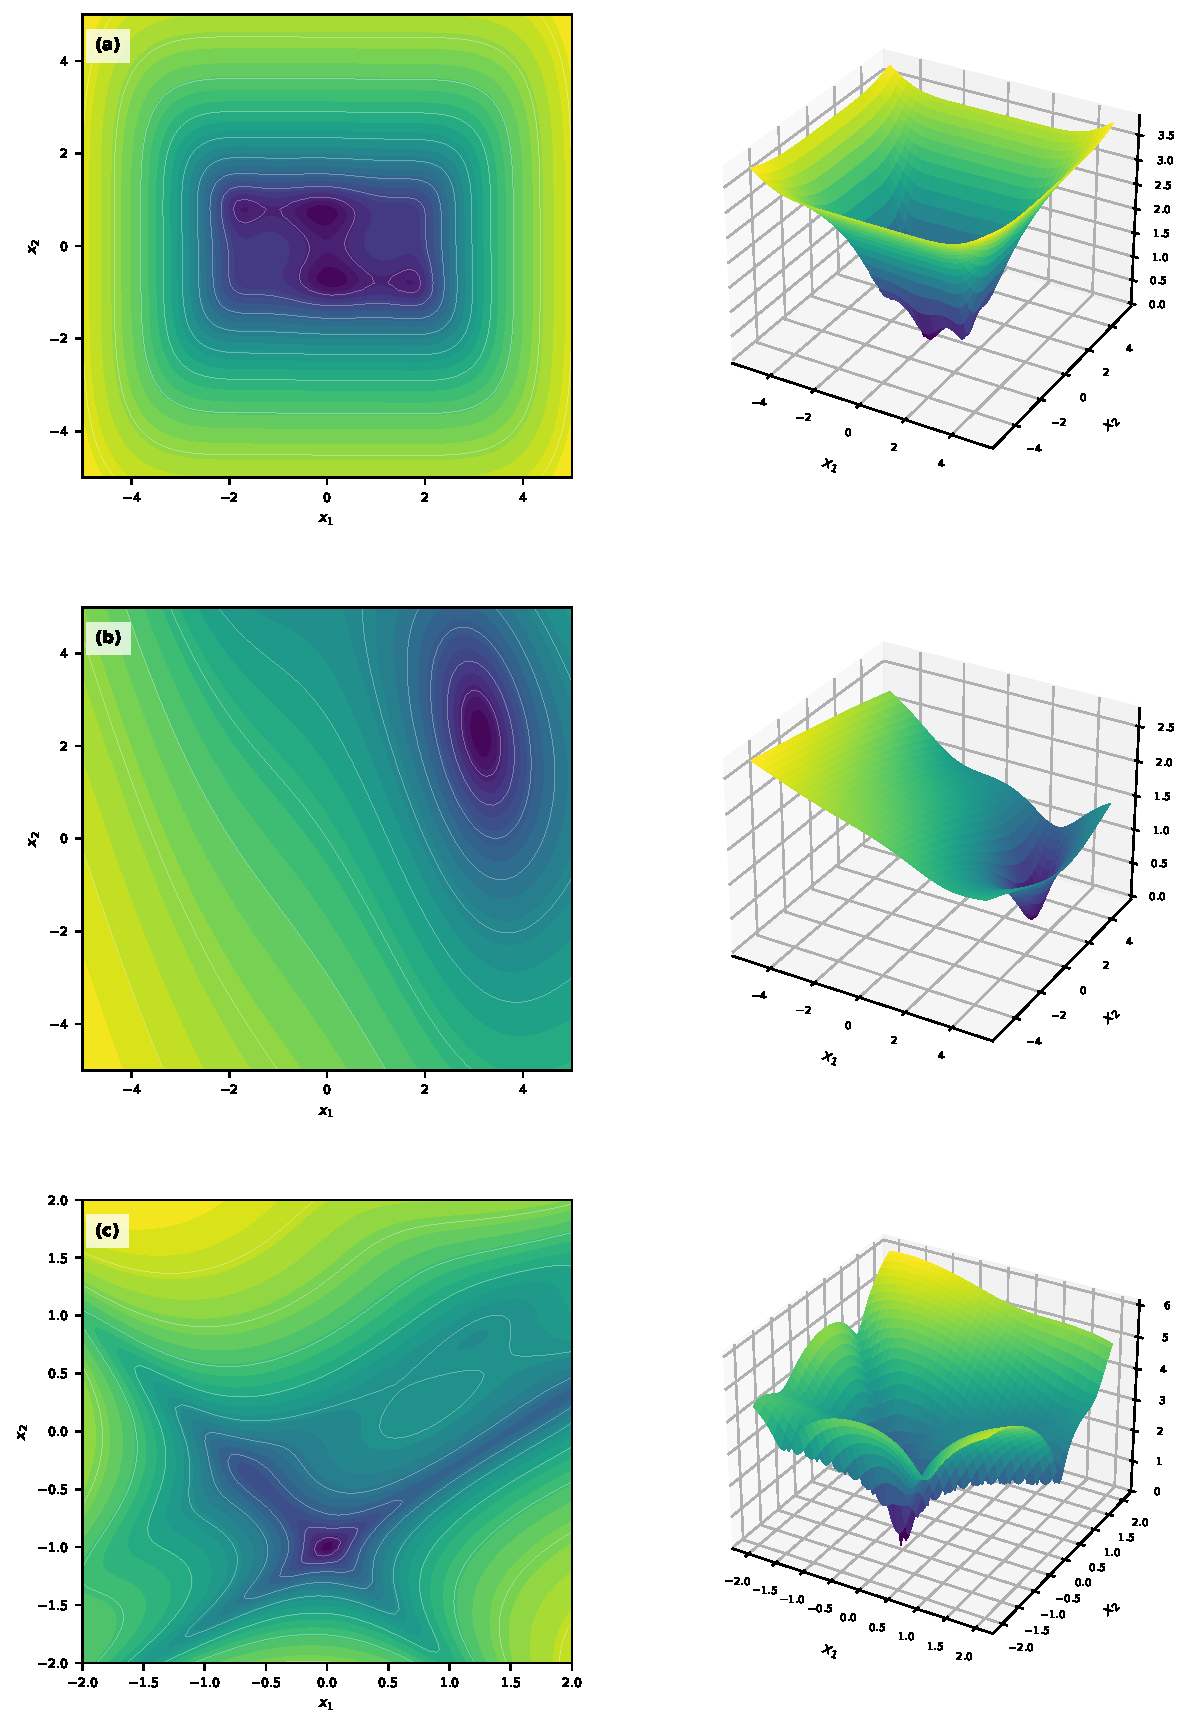
\includegraphics[width=\fulllength,height=0.84\textheight,keepaspectratio]{figures/landscapes_body/landscape_body_group_06.pdf}
  \end{adjustwidth}
  \caption{Benchmark objective landscapes and two-dimensional slices: (a) F16 (Six-hump camel, $d=2$); (b) F17 (Branin, $d=2$); (c) F18 (Goldstein-Price, $d=2$). Contours are shown at left and 3-D surfaces at right; colour shows log-compressed objective excess on function-specific scales. For $d>2$, other coordinates are fixed at the midpoint of the solver bounds. Bounds and reference optima are listed in Tables~\ref{tab:benchmark_scalable}--\ref{tab:benchmark_fixed}.}
  \label{fig:landscape_body_06}
\end{figure}
\clearpage

\begin{figure}[p]
  \begin{adjustwidth}{-\extralength}{0cm}
  \centering
  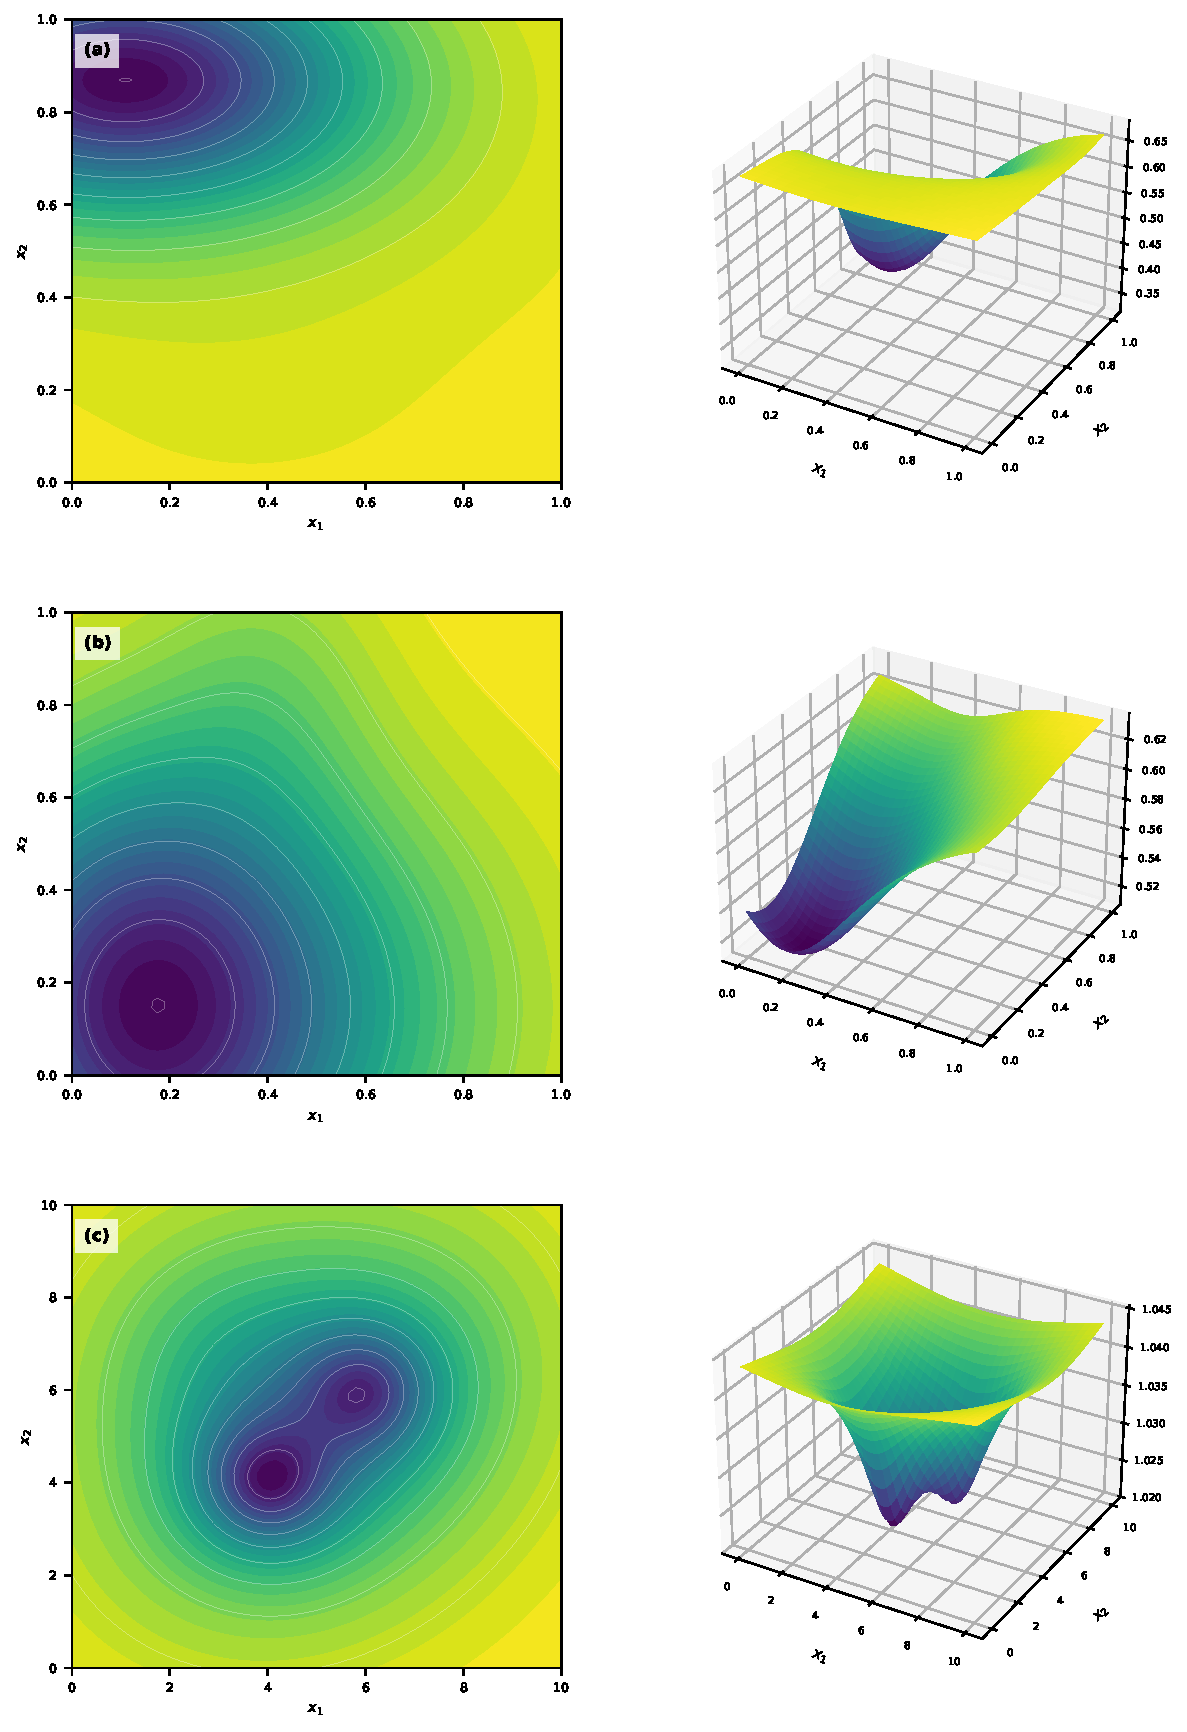
\includegraphics[width=\fulllength,height=0.84\textheight,keepaspectratio]{figures/landscapes_body/landscape_body_group_07.pdf}
  \end{adjustwidth}
  \caption{Benchmark objective landscapes and two-dimensional slices: (a) F19 (Hartmann 3-D, $d=3$); (b) F20 (Hartmann 6-D, $d=6$); (c) F21 (Shekel-5, $d=4$). Contours are shown at left and 3-D surfaces at right; colour shows log-compressed objective excess on function-specific scales. For $d>2$, other coordinates are fixed at the midpoint of the solver bounds. Bounds and reference optima are listed in Tables~\ref{tab:benchmark_scalable}--\ref{tab:benchmark_fixed}.}
  \label{fig:landscape_body_07}
\end{figure}
\clearpage

\begin{figure}[p]
  \begin{adjustwidth}{-\extralength}{0cm}
  \centering
  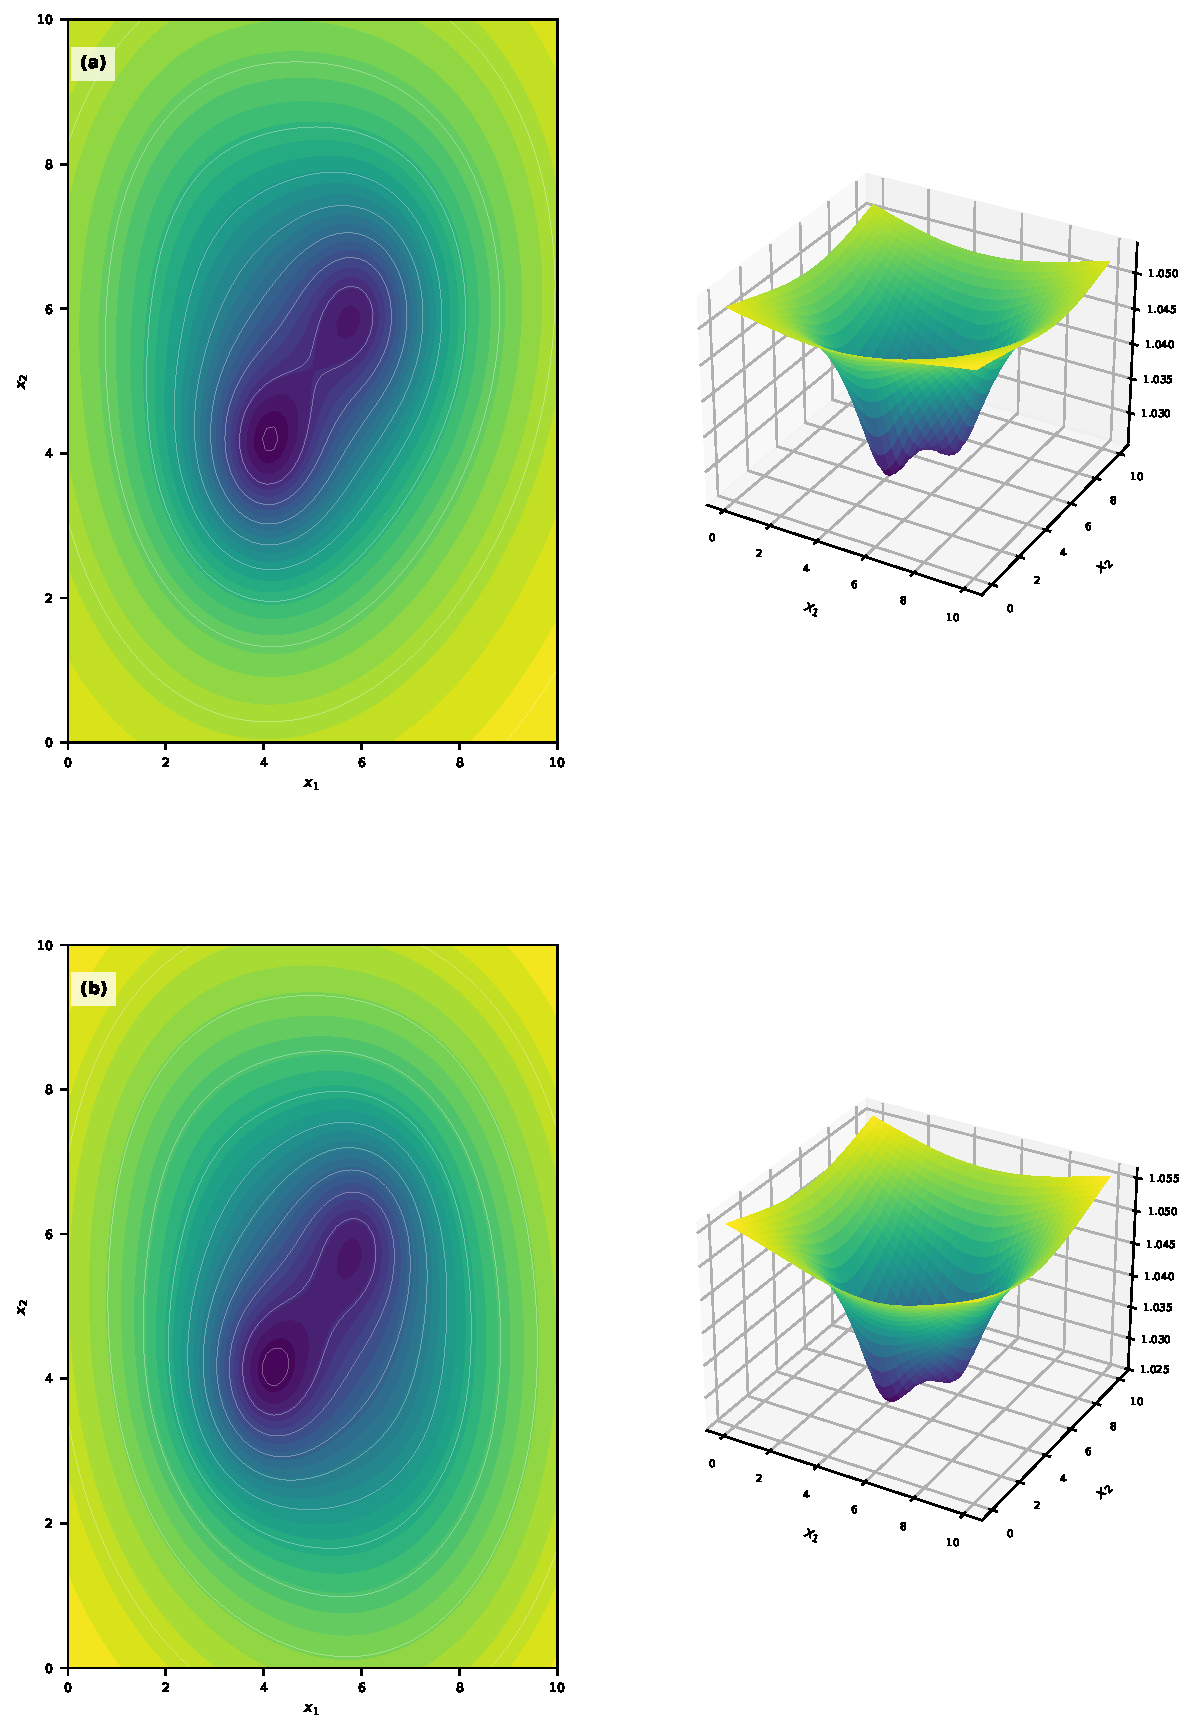
\includegraphics[width=\fulllength,height=0.84\textheight,keepaspectratio]{figures/landscapes_body/landscape_body_group_08.pdf}
  \end{adjustwidth}
  \caption{Benchmark objective landscapes and two-dimensional slices: (a) F22 (Shekel-7, $d=4$); (b) F23 (Shekel-10, $d=4$). Contours are shown at left and 3-D surfaces at right; colour shows log-compressed objective excess on function-specific scales. For $d>2$, other coordinates are fixed at the midpoint of the solver bounds. Bounds and reference optima are listed in Tables~\ref{tab:benchmark_scalable}--\ref{tab:benchmark_fixed}.}
  \label{fig:landscape_body_08}
\end{figure}
\clearpage


\authorcontributions{Conceptualization, J.B.-G., B.C., F.C.-C., 
Methodology, J.B.-G., B.C., J.G.-P., Software, J.B.-G., F.C.-C., Y.L., 
Validation, J.B.-G., B.C., J.G.-P.,F.C.-C., Y.L., A.P., Á.P.F., R.S., 
Formal analysis, J.B.-G., F.C.-C., Y.L., A.P., Á.P.F., 
Investigation, J.B.-G., F.C.-C., Y.L., 
Resources, B.C., A.P., Á.P.F., 
Data curation, J.B.-G., F.C.-C., Y.L., 
Writing -- original draft, J.B.-G., F.C.-C., Y.L., 
Writing -- review \& editing, J.B.-G., B.C., J.G.-P.,F.C.-C., Y.L., A.P., Á.P.F., R.S., 
Visualization, J.B.-G., F.C.-C., Y.L., A.P., Á.P.F., 
Supervision, B.C., J.G.-P.,R.S., 
Project administration, B.C., J.G.-P.,R.S.}

\funding{This research received no external funding.}
\dataavailability{The consolidated run-level dataset, including the verified run seeds, and the machine-readable statistical summaries supporting the findings are provided in the Supplementary Materials.}

% DO NOT CHANGE THE ACKNOWLEDGMENTS SECTION
\acknowledgments{José Barrera-García is supported by the National Agency for Research and Development (ANID)/Scholarship Program/DOCTORADO NACIONAL/2024-21242516. Broderick Crawford is supported by Grant ANID/FONDECYT/REGULAR/1262511.
}

\conflictsofinterest{The authors declare no conflicts of interest.}

% \abbreviations{Abbreviations}{
% The following abbreviations are used in this manuscript:\\

% \noindent
% \begin{tabular}{@{}ll}
% PSO & Particle Swarm Optimization\\
% FCS & Fuzzy Control System\\
% FIS & Fuzzy Inference System\\
% XPL & Exploration percentage (current diversity relative to its running maximum)\\
% \end{tabular}
% }

%=================================================================
\begin{adjustwidth}{-\extralength}{0cm}

\reftitle{References}

\bibliography{refs}

\end{adjustwidth}

\end{document}
